%
% Modified by Megan Patnott
% Last Change: Jan 18, 2013
%
%%%%%%%%%%%%%%%%%%%%%%%%%%%%%%%%%%%%%%%%%%%%%%%%%%%%%%%%%%%%%%%%%%%%%%%%
%
% Modified version of the sample_ndthesis.tex
% by Sameer Vijay
% Last Change: Wed Jul 27 2005 14:00 CEST
%
%%%%%%%%%%%%%%%%%%%%%%%%%%%%%%%%%%%%%%%%%%%%%%%%%%%%%%%%%%%%%%%%%%%%%%%%
%
% Sample Notre Dame Thesis/Dissertation
% Using Donald Peterson's ndthesis classfile
%
% Written by Jeff Squyres and Don Peterson
%
% Provided by the Information Technology Committee of
%   the Graduate Student Union
%   http://www.gsu.nd.edu/
%
% Nothing in this document is serious except the format.  :-)
%
%%%%%%%%%%%%%%%%%%%%%%%%%%%%%%%%%%%%%%%%%%%%%%%%%%%%%%%%%%%%%%%%%%%%%%%%
% This is *not* a substitute for the documentation, which is included
% as a pdf file in the standard distribution, and can be obatined from
% the dtx file in the advanced distribution.
%%%%%%%%%%%%%%%%%%%%%%%%%%%%%%%%%%%%%%%%%%%%%%%%%%%%%%%%%%%%%%%%%%%%%%%%
%
% You should *also* have a ND formatting guide to ensure that you have
% all the relevant parts, put the captions in the right place, etc.
% Just because you have this wonderful style classfile doesn't mean
% that it removes *all* the formatting onus from you.  :-)
% Although be warned that the Graduate School has been known to let
% their official formatting guide get out of date. When in doubt,
% the Microsoft Word example seemed to be the only thing kept
% consistently up-to-date in 2013, and is probably the safest thing
% to consult.
%
% You should break all of this stuff up into separate files
% (at the very least, one chapter per file) and use the \include
% command, as has been done here for chapters 1 and 2 and the appendix.
% There is also an \input command, but \include is more commonly used to
% import chapters in books and dissertations. For the differences between these
% two commands, see, e.g., 
% http://web.science.mq.edu.au/~rdale/resources/writingnotes/latexstruct.html
% or http://tex.stackexchange.com/questions/246/when-should-i-use-input-vs-include.
%
% If you compile from the command line, note that you should also have 
% a good Makefile; one that invokes LaTeX as many times as necessary 
% (up to 4) and bibtex if necessary.
%
% If you use an editor that allows you to compile from within the
% program, note that you will need to compile up to four times. Also,
% we recommend that you use pdflatex (sometimes displayed as
% LaTeX => PDF) to compile directly to pdf.
%
% If you have any suggestions, comments, questions, please send e-mail
% to: dteditor@nd.edu
%
%%%%%%%%%%%%%%%%%%%%%%%%%%%%%%%%%%%%%%%%%%%%%%%%%%%%%%%%%%%%%%%%%%%%%%%%

\documentclass[final,numrefs,sort&compress,noinfo]{nddiss2e}
% One of the options draft, review, final must be chosen.
% One of the options textrefs or numrefs should be chosen
% to specify if you want numerical or ``author-date''
% style citations.
% Other available options are:
% 10pt/11pt/12pt (available with draft only)
% twoadvisors
% noinfo (should be used when you compile the final time
%         for formal submission)
% sort (sorts multiple citations in the order that they're
%       listed in the bibliography)
% compress (compresses numerical citations, e.g. [1,2,3]
%           becomes [1-3]; has no effect when used with
%           the textrefs option)
% sort&compress (sorts and compresses numerical citations;
%           is identical to sort when used with textrefs)


\begin{document}

\frontmatter % All the items before the first chapter go in ``frontmatter''

% Titles may be 1-4 lines long. If your title is longer than 4 lines,
% the class file may have difficulty formatting the title page.
% Line-breaks in the title have to be protected with `\protect`.
\title{Conversion Electrons in $^{154,156}$Gd}
\author{Sabrina Yve Strauss}
\work{Dissertation} % or \work{Thesis}
%\degaward{Doctor of Philosophy} % or 
\degaward{Doctorate of Philosophy \\ in \\ Physics}
\advisor{Ani Aprahamian}
\department{Physics}

\maketitle
%%%%%%%%%%%%%%%%%%%%%%%%%%%%%%%%%%%%%%%%%%%%%%%%%%%%%%%%%%%%%%%%%%%%%%%%
%
% Front stuff
%
%%%%%%%%%%%%%%%%%%%%%%%%%%%%%%%%%%%%%%%%%%%%%%%%%%%%%%%%%%%%%%%%%%%%%%%%

% You must either set the copyright information or put your work in the public domain.
\copyrightholder{Sabrina Strauss} % See template or documentation for
\copyrightyear{2018}           % other copyright options.
\copyrightlicense{CC-BY-4.0}
\makecopyright

% An abstract is optional for a master's thesis, and required for a doctoral dissertation.
\begin{abstract}
    E0 components of transitions between two states of the same spin and parity are challenging to measure, with sparse information available in nuclear databases. A recent study of $^{154}$Gd (D. A. Meyer et al, PRC 044309(2006)) showed the nucleus to have 16 0$^+$ states. $^{154}$Gd is well-studied by a number of reactions, hence it is an ideal candidate to search for E0 transitions. We will report on our results for transitions in $^{154}$Gd following the $^{152}$Sm($\alpha$,2n) reaction using the Internal Conversion Electron Ball (ICEBall) array in coincidence with $\gamma$-rays at the University of Notre Dame Nuclear Science Laboratory (NSL). ICEBall was re-implemented at the NSL 4 years ago and the $\gamma$-rays were detected by Clovershare, segmented HPGe detectors purchased by the Yale Nuclear Structure Laboratory that are shared by a consortium of universities and laboratories for experimental campaigns.
\end{abstract}

% A dedication is optional.
\renewcommand{\dedicationname}{To my parents, who always encouraged my love of science.\\
To Jolie, who introduced me to nuclear physics research.\\
To Ani, who helped keep me from going too far down side paths. \\
To all the people who put up with my mood swings.}

\centering{\dedicationname}

\raggedright

% These are required, and must be in this order.
\tableofcontents
\listoffigures
\listoftables

% A preface is optional.
\begin{preface}
\end{preface}

% It's hard to tell from the information available from the Graduate
% School in Spring 2013 whether or not an acknowledgements section is optional.
\begin{acknowledge}
\end{acknowledge}

\mainmatter
%
% Chapter 1
%

%
% Chapter 1
%

\chapter{Introduction}

% What is matter?
Visible matter comprises $\sim$5 percent of the universe. This matter makes up all living things and ecosystems, including the stars and planets. This matter exists entirely within the atom, with the nucleus holding more than 99.9 \% of all matter. The nucleus is comprised of protons and neutrons in different configurations, held together by the strong force. Understanding this essential building block of the universe is at the heart of understanding how matter is formed and evolves.

The periodicity of phenomena on the atomic level and higher is well documented near stability, from the lattice structures of crystals, to the periodic table of the elements, organized in a way that groups elements that behave similarly due to the structure of the orbiting atomic electrons. The periodic table organizes elements based on similar properties, such as the halogens and noble gases. The elements can be neatly grouped by similar chemical properties. But, this periodic table does not delve into the subatomic level. The periodic table separates out atoms by the number of protons, which equates with the atomic number, but the number of neutrons in a nucleus can also vary, creating different isotopes of an element that is otherwise chemically identical. When mapping these two, we create Figure \ref{fig:chart}, known as the chart of nuclides. These nucleons are held together by the strong force, which has a short range. In the low-mass region of the chart, this creates a linear trend for the line of stability. As mass and the total number of nucleons increases, the line of stability trends toward the neutron side, due to repulsion by the coulomb force in the protons. As the neutrons do not contribute significantly to the coulomb force, the addition of more neutrons creates larger separation between protons, decreasing the coulomb contribution.

\begin{figure}
    \centering
    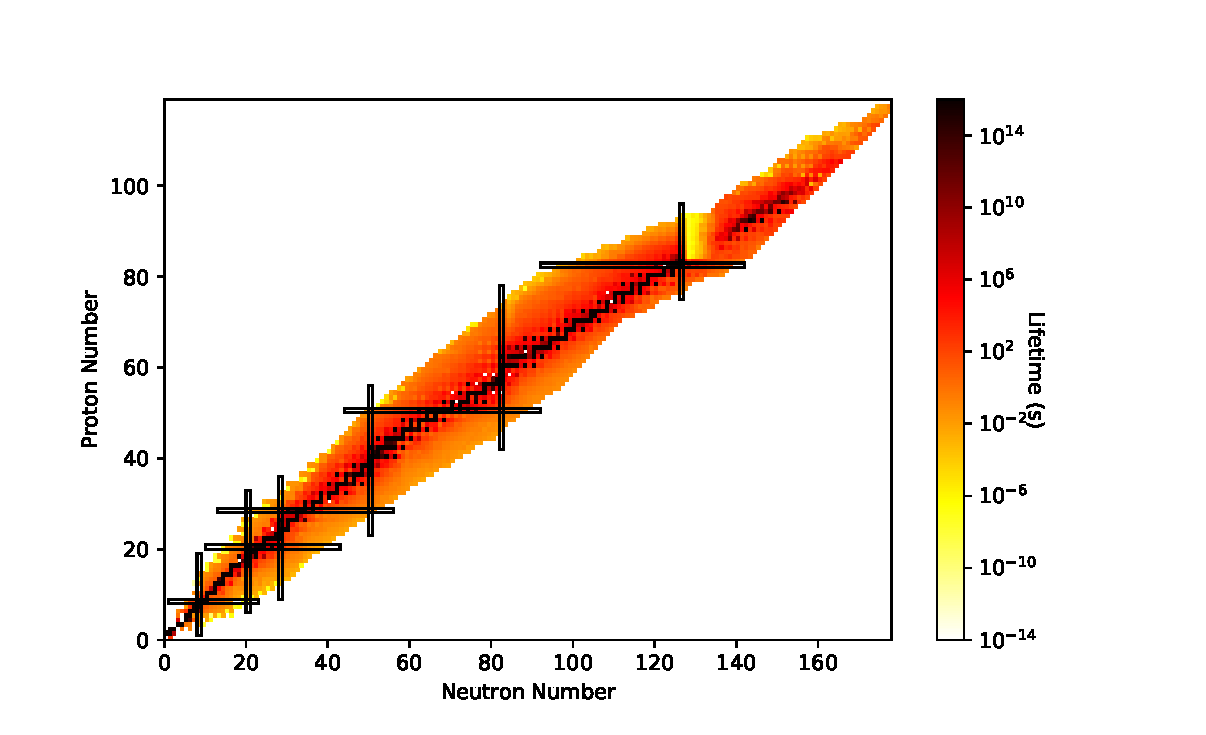
\includegraphics[scale=0.8]{Introduction_Figs/ChartNuclides.eps}
    \caption{The chart of nuclides. The $x$-axis is increasing in neutron number from left to right, and the $y$-axis is increasing in proton number from bottom to top. The lower leftmost corner is the lightest elements, while the upper right are the heaviest, including superheavy elements. Black boxes indicate stable or extremely long lived nuclei. These nuclei are in the "center" of the chart, and known colloquially as the valley of stability. To either side of these stable nuclei are radioactive nuclei, which become shorter lived the farther they are from the valley, indicated by the lightening color. The black boxes are at neutron and proton numbers 8, 20, 28, 50, 82 and 126, marking closed shells for spherical nuclei, and are discussed in further depth within the text.}
    \label{fig:chart}
\end{figure}

The chart of nuclides has several notable features in this form. The color coding in Figure \ref{fig:chart} is representative of the lifetimes of the isotopes represented in each box: lighter boxes are shorter-lived, while darker boxes are longer lived, with black boxes being stable isotopes. This creates a black line going up at approximately $N=Z$, known as the valley of stability. Additionally in this figure, several rows and columns are singled out. These rows and columns are a series of numbers referred to as the "magic" numbers, and highlight a form of periodicity in nuclei. 

This periodic nature is explained through the shell model. Based on the same idea as atomic electrons, the "shells" occur due to the energy gap in levels. The neutrons and protons each have separate potential wells and levels populated. When examining solutions to this potential well, the magic numbers naturally form after including angular momentum, and taking the spin-orbit interaction into account, as seen in Figure \ref{fig:shellmodel}. These magic numbers represent closed shells of a spherical nucleus model. It is of note, that a doubly-magic nucleus, that is, a nucleus with both neutron and proton close shells, is spherical. However, a nucleus with only a single closed shell is not, necessarily, spherical. These closed shells cause a variety of effects, including high energy of the first excited $2^+$ state at closed shells, seen in Figure \ref{fig:E2bymass}. The high energy of the first excited $2^+$ state near the closed shells is due to the large energy gaps that occur at closed shells, seen on the right side of Figure \ref{fig:shellmodel}.
 %, and the low reduced transition rate between this first excited state and the ground state, seen in Figure \ref{fig:reducedtrans}. 

\begin{figure}
    \centering
    \includegraphics[scale=2]{Introduction_Figs/ShellBreakdownCasten.png}
    \caption{The evolution of the shel model and the creation of the closed shells of a spherical nucleus. On the left is the spherical harmonic oscillator. By adding in an angular momentum term, some of the degenerate levels separate. By further adding a spin-coupling term, the levels separate with energy spacings that create the closed shells and the magic numbers. Taken from \citep{casten90:_structure}.}
    \label{fig:shellmodel}
\end{figure}

\begin{figure}[!]
    \centering
    \includegraphics[scale=2]{Introduction_Figs/E2byMassCasten.png}
    \caption{The energy of the first excited $2^+$ state, plotted in isotopic chains, by mass. Areas of high excitation energy, around A$\sim$90,140,210 all correspond to doubly magic areas. The areas around A$\sim$110,170 have much lower excitation energies and correspond to areas of deformation.  Taken from \citep{casten90:_structure}}
    \label{fig:E2bymass}
\end{figure}

% \begin{figure}
    \centering
    \includegraphics[scale=2]{Introduction_Figs/ReducedTransbyMassCasten.png}
    \caption{A plot of the reduced transition rate between the first excited $2^+$ state and the ground state in even-even nuclei, in single particle units. Areas of low rates, around A$\sim$90,140,210, correspond to closed shells, while the areas around A$\sim$110,170,250, have much higher rates, and correspond to deformed nuclei. Taken from \citep{casten90:_structure}.}
    \label{fig:reducedtrans}
\end{figure}

Outside of these closed shells, there are large regions that do not work within the paradigm created by this phenomenon. Nuclei near the close shells are generally expected to be spherical in nature. However, the shell model becomes extremely complex away from the closed shells. In some cases, the magic numbers themselves appear to change. This change can be charted using the Nilsson model, which evolves the spherical shell model as it deforms into an ellipsoid. The model uses the deformation parameter $\beta$ in the hamiltonian, allowing the level energies to be seen as a function of $\beta$. This leads to a collapse and change of the magic numbers, as seen in Figure \ref{fig:nilsson}.

\begin{figure}
    \centering
    \includegraphics{Introduction_Figs/nilsson.jpg}
    \caption{The Nilsson diagram, showing the evolution of the shell levels of the nucleus with respect to the deformation parameter $\beta$. As the nucleus gets more deformed, the closed shells break down. Taken from \citep{choppin13:_nilsson}.}
    \label{fig:nilsson}
\end{figure}

In the area around $Z=60$ and $N=90$, away from the closed shells, nuclei do not hold a spherical shape. They lose symmetry on the major axes, becoming axially assymmetric. /i/e/ $x=y\neq z$ or $x \neq y \neq z$. The former case has two forms: oblate (pancake-like) or prolate (football-like) depending on whether the nucleus appears compressed (oblate) or elongated (prolate) along the symmetry axis ($z$), as seen in Figure \ref{fig:deformation}. In Figure \ref{fig:nilsson}, the negative $\beta$ corresponds to oblate nuclei, while positive $\beta$ corresponds to prolate nuclei. There are more exotic deformations when the latter assymmetry is true, where symmetry is broken along two or more axes, resulting in pear-shapes and other exotic formations.

\begin{figure}
    \centering
    \includegraphics[scale=1]{Introduction_Figs/Deformation.png}
    \caption{Illustration of different kinds of deformation, where spherical symmetry is lost. Treating the vertical as the axis of symmetry, the prolate nucleus is contracted along this axis, but is still axially symmetric. The oblate nucleus is elongated along this axis, but otherwise axially symmetric. It is also possible for the nucleus to lose axial symmetry.}
    \label{fig:deformation}
\end{figure}

There are several ways to look for deformation in a nucleus. The most common is the quadrupole moment, which is directly related to the quadrupole deformation parameter, $\beta_2$ (also referred to as $\beta$) by

\begin{equation}
    Q_0 = \frac{3}{\sqrt{5\pi}}ZR_0^2\beta_2\left(1+0.16\beta_2\right)
\end{equation}

to second order, where $Z$ is the atomic number, and $R_0$ is the approximate radius based on $R_0=1.2A^{1/3}$fm, where $A$ is the number of nucleons \citep{casten90:_structure}. This can be measured in even-even nuclei using the transition between the first excited $2^+$ state and the $0^+$ ground state. The onset of deformation can be seen in Figure \ref{fig:beta_by_isotope}, via the rapid increase in $\beta_2$. The equation used to calculate $\beta_2$ for this figure is 

\begin{equation}
    \beta_2 = \frac{4\pi}{3ZR^2_0}\left[B(E2)\right]^{1/2}
\end{equation}

where B(E2) is the reduced transition probability for the $0^+_1\rightarrow2^+_1$ transition. There is no way to distinguish prolate and oblate using this calculation, as the sign comes from the choice of sign on the root. The choice cannot be decided with the information in the equation.

\begin{figure}
    \centering
    \includegraphics[scale=2]{Introduction_Figs/DeformationParamCasten.png}
    \caption{Plot of the deformation parameter $\beta_2$ along isotopic chains. Deformation can be seen setting in, as isotopic chains transition from spherical to deformed. The formula to calculate $\beta_2$ from the reduced transition probability is shown. This $\beta_2$, is an absolute measure of deformation, and does not distinguish between prolate and oblate. Taken from \citep{casten90:_structure}.}
    \label{fig:beta_by_isotope}
\end{figure}

In the lanthanide region, there are multiple stable isotopes of several elements, including samarium ($Z=62$) and gadolinium ($Z=64$). Studies across these elements show the onset of deformation through systematics like the energy of the first excited $2^+$ state, and the ratio between the energies of the first $4^+$ and $2^+$ excited states, seen in Figure \ref{fig:E4E2}. The $E_{4^+_1}/E_{2^+_1}$ ratio theoretically tops out at 3.3. This ratio gives a measure of the moment of inertia of the ground-state band of the nucleus, as, for a rigid rotor,

\begin{equation}
    E=\frac{\hbar^2}{2\mathscr{J}_{eff}}J(J+1)
\end{equation}

The moment of inertia, $\mathscr{J}_{eff}$, varies as energy increases. In a perfect rigid rotor, this would not be the case, and $\mathscr{J}_{eff}=\mathscr{J}_{rigid}=\frac{2}{5}Am_{\mathscr{N}}r_0^2A^{2/3}$. Taking the ratio of two energy levels, $J=4$ and $J=2$ in this case, would give a ratio of 10/3, or 3.3. However, if it is not a rigid rotor, this number deviates from 3.3, as the change in the effective moment of inertia changes. The model used by Bohr and Mottelson shows that $\mathscr{J}_{eff}$ is proportional to the square of the deformation parameter, $\beta_2$, at low deformation, and approaches that of a rigid body at high deformation \citep{bohr55:_deformation}.

\begin{figure}
    \centering
    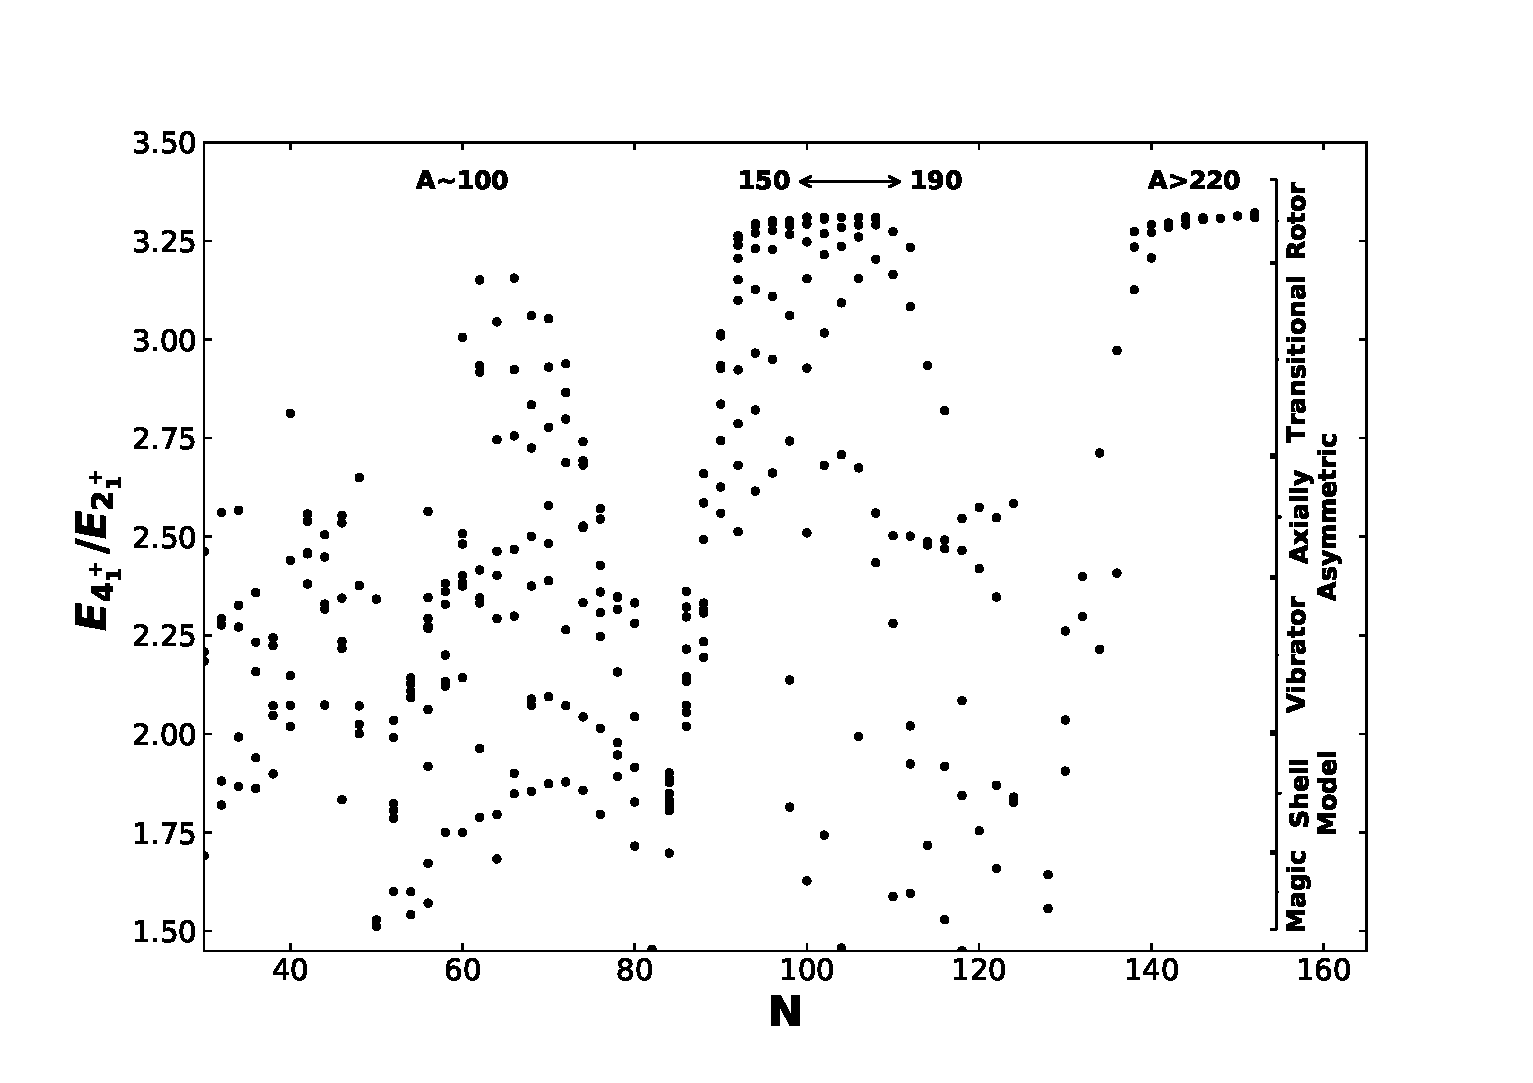
\includegraphics[scale=0.6]{Introduction_Figs/E4E2ratiovsN.eps}
    \caption{Plot of the ratio of the first $4^+$ excited state energy to the first $2^+$ excited state energy in even-even nuclei. On the right, the ratio is broken down into sections, based on structure. This ratio is an excellent diagnostic of the general nuclear structure.}
    \label{fig:E4E2}
\end{figure}

Much of these nuclei are successfully modelled with deformation in theoretical calculations \citep{delaroche10:_systematics}. These models can also open up new questions, when a previously identified feature does not fit with the assignment in an otherwise well described system.

\section{Nuclear Excitations}
\label{sec:nuc_excite}

There are many different ways a nucleus can be excited. While the types of excitations available depend on shape, there are two extremes to consider: a single particle excitation, and a collective excitation. The single particle excitation can be described as a single neutron, proton, or hole from a closed shell being excited to a different level. A collective excitation is usually thought of on a macroscopic level, looking at large numbers of nucleons moving together. These are only extremes, and there are excitations that can be described as multi-particle that would fit in-between. All of these excitations can exist within a nucleus.

\subsection{Collective Excitations}

Two types of collective excitations are rotational and vibrational excitations. Rotational excitations occur in deformed nuclei, as discussed earlier, where spherical symmetry is broken, i.e. $x=y\neq z$ or $x \neq y \neq z$. These are caused by the rotation of the nucleus about the axis of symmetry. Vibrational excitations involve the compression and expansion of the nucleus as a whole. These come in different modes, and have a characteristic even spacing, seen in Figure \ref{fig:statestructure}.

\begin{figure}
    \centering
    \includegraphics[scale=2]{Introduction_Figs/EvolutionofStructureCasten.png}
    \caption{Cartoon of what excited states built upon different types of nuclei looks like. The closed shell has a large gap between the ground state and first excited state. In the vibrator model, this gap is lower, and a gap of comparable size exists before a cluster of states occurs. In the rotor model, the spacing follows a spacing pattern of $J_f(J_f+1)-J_i(J_i+1)$, with $\gamma$ and $\beta$ vibrations also coming into play. The trasitional area between vibrator and rotor shows a shift between the two, with the clustered states of the vibrator model beginning to space out. Taken from \citep{casten90:_structure}.}
    \label{fig:statestructure}
\end{figure}

There are several ways to tell the difference between these types of excitations. The collective models have well-described spacing of the levels, seen in Figure \ref{fig:statestructure}. Vibrational excitations will be spaced regularly as $n\hbar\omega$, while rotational excitations will have increasing spacing between the levels as $J$ increases. The reduced transition probabilities also give information about the difference between two different levels. The single-particle strengths for these transitions can be calculated and are known as Weisskopf estimates. The reduced transition probability can then be written in Weisskopf units using the estimate, which gives a measure of the collectivity of the transition. This does have limitations, however, as the Weisskopf estimate assumes a spherical nuclear model.

\subsection{Shape Coexistence}

Another aspect of nuclear shape is that of shape coexistence. In shape coexistence, there is more than one minima of the potential well, at different forms of deformation, as illustrated in Figure \ref{fig:shape}. These two minima represent two different shapes of the nucleus, and both can have excitations built upon them. The two shapes can also interact, causing shape mixing effects. 

\begin{figure}
    \centering
    \includegraphics[scale=0.5]{Introduction_Figs/ShapeCoexist.png}
    \caption{Cartoon of the potential well of a nucleus with shape coexistence. A second minima appears at a different $\beta$, the deformation parameter. Both of these minima can have excitations built on top of them, leading to shape coexistence.}
    \label{fig:shape}
\end{figure}

There are two main theoretical approaches to shape coexistence in nuclei: microscopic shell-model and mean-field descriptions \citep{heyde11:_shape_coexist}. These two approaches compliment each other. In the shell-model approach, a spherical shell model is assumed, and particle-hole excitations across closed shells are examined. For an $n$p-$n$h configuration, it would appear the $0^+$ states are too high. However, upon correcting for monopole interaction energy, and then coupling different $n$p-$n$h subspaces together, lower energy $0^+$ states are calculated \citep{caurier07:_shape_coexist}. For calculations above $A=80$, nucleons must be treated in pairs built from realistic collective pairs, as the model spaces become too large for current computational power\citep{heyde11:_shape_coexist}. In this approach, intruder states from even-even particle-hole excitations can create shape-coexisting $0^+$ states.

The mean-field approach uses the self-consistent Hartree-Fock-Bogoliubov (HFB) theory. The effective forces are tuned to describe global nuclear properties. When minimizing the energy, deformation in the nuclear shape can result. Various mean-field states are found, which have broken symmetries needed within the nucleus. These states are projected onto the proper particle numbers, isospin, and angular momentum to produce the physical states observed \citep{heyde11:_shape_coexist}. To compare with experimental date, the Hamiltonian must be rediagonlized in terms of the physical, projected states.

Shape coexistence, like the collective excitations, has spectroscopic fingerprints that can help determine its existence. As with deformation, large reduced transition rates are a possible sign of shape coexistence, but do not distinguish between static and dynamic deformation \citep{heyde11:_shape_coexist}. The diagonal $E2$ matrix elements can distinguish between the dynamic and static. The $E0$ transitions present in $J^{\pi}\rightarrow J^{\pi}$ may also be an indirect fingerprint of shape coexistence, as it is related to the change in the mean radius of the nucleus, as discussed in Section \ref{sec:E0}\citep{wood99:_e0}. The low-lying states of interest can be difficult to observe, as they are not populated strongly in reactions.

\section{Multipole Radiation}
\label{sec:multipole}
When the nucleus is in an excited state, with energy in excess of its ground state, this excess is stored in the protons and neutrons of the nucleus. These nuclei oscillate, creating electromagnetic fields with their oscillation. The nucleus is then capable of deexciting in different ways. With enough energy, the nucleus will preferentially emit particles, such as neutrons or protons. To do so, it must be at a high enough energy. In the case that enough energy is not present for particle emission, the electromagnetic force becoming the route of de-excitation, via photon emission in the form of $\gamma$-rays. These fields are commonly described using expansions of spherical harmonics, allowing for angular momentum identification of the radiation emitted. This expansion is commonly referred to as multipole expansion. Discussion and derivation can be found in detail in many references \citep{blatt79:_emradiation, jackson99:_emradiation, zangwill13:_emradiation}.

The Maxwell equations are
\begin{subequations}
\label{eq:maxwell_free}
\begin{align}
    \nabla \cdot \textbf{E} & = 0 &   \nabla \times \textbf{E} & = -\frac{\partial \textbf{B}}{\partial t} \\
     \nabla \cdot \textbf{B} & = 0 &  \nabla \times \textbf{B} & = \frac{1}{c^2}\frac{\partial \textbf{E}}{\partial t}
\end{align}
\end{subequations}
for a vacuum with no source. Radiation from a nuclear transition has a well-defined energy, and therefore, a well-defined frequency $\omega$. The time-dependence of the electric and magnetic field can be expressed as
\begin{subequations}
\label{eq:maxwell_rad}
\begin{align}
    \textbf{E}(\textbf{r},t) & = Re\left\{\textbf{E}(\textbf{r},t)e^{-i\omega t}\right\} \\
    \textbf{B}(\textbf{r},t) & = Re\left\{\textbf{B}(\textbf{r},t)e^{-i\omega t}\right\}
\end{align}
\end{subequations}
 
Using equations \ref{eq:maxwell_free} and \ref{eq:maxwell_rad}, the Maxwell equations can be rewritten in the equivalent forms
\begin{subequations}
\label{eq:maxwell_rw1}
\begin{gather}
    \left(\nabla^2+k^2\right)\textbf{E} = 0 \\
    \nabla \cdot \textbf{E} = 0 \\
    \textbf{B}=-\frac{i}{ck} \nabla \times \textbf{E}
\end{gather}
\end{subequations}
and
\begin{subequations}
\label{eq:maxwell_rw2}
\begin{gather}
    \left(\nabla^2+k^2\right)\textbf{B} = 0 \\
    \nabla \cdot \textbf{B} = 0 \\
    \textbf{E}=-\frac{ic}{k} \nabla \times \textbf{B}
\end{gather}
\end{subequations}

As these are equivalent, any pair of fields \textbf{B}(\textbf{r}) and \textbf{E}(\textbf{r}) that satisfy equations \ref{eq:maxwell_rw1} must satisfy equations \ref{eq:maxwell_rw2} and vice-versa. It can be shown that any arbitrary solution to the Maxwell equations can be written as a linear combination of a transverse magnetic wave and a tranverse electric wave, i.e. 
\begin{align}
    \label{eq:trans_E}
    \textbf{r} \cdot \textbf{E} & = 0, \text{ or} \\
    \label{eq:trans_B}
    \textbf{r} \cdot \textbf{B} & = 0
\end{align}

When combining equations \ref{eq:trans_E} and \ref{eq:maxwell_rw1}, a solution to the Maxwell equations can be derived. When doing the same with equations \ref{eq:trans_B} and \ref{eq:maxwell_rw2}, a separate, linearly independent, solution can be derived. These two solutions in combination can express any of the solutions to the Maxwell equations as a linear combination.

Because of the linear independence of the spherical harmonics, solutions to these wave equations can be written as multipole expansions, the term multipole in reference to the angular momentum, $l$, defining the series of the harmonic. The first set of solutions give the magnetic multipole fields, with the solutions
\begin{subequations}
\label{eq:magnetic_sol}
\begin{align}
    \left(\nabla^2+k^2\right)\textbf{E}^\text{M} & = 0 & \textbf{B}^\text{M}=-\frac{i}{ck} \nabla \times \textbf{E}^\text{M} \\
    \nabla \cdot \textbf{E}^\text{M} & = 0 & \textbf{r}\cdot\textbf{E}^\text{M}=0
\end{align}
\end{subequations}
where the M indicates the magnetic multipole component of the field. The second set give the electric multipole fields with the solutions
\begin{subequations}
\label{eq:electric_sol}
\begin{align}
    \left(\nabla^2+k^2\right)\textbf{B}^\text{E} & = 0 & \textbf{E}^\text{E}=-\frac{ic}{k} \nabla \times \textbf{B}^\text{E} \\
    \nabla \cdot \textbf{B}^\text{E} & = 0 & \textbf{r}\cdot\textbf{B}^\text{E}=0
\end{align}
\end{subequations}
where the E indicates the electric multipole component of the field. The total fields are then just the two components summed together.

These multipole fields can be written as an expansion of the spherical Hankel functions, $h_l^{1,2}(kr)$, multiplied by the spherical harmonics, $Y_{lm}(\theta,\phi)$. The fields can then be broken apart into components of $l$, the angular momentum.  The general expressions for $\textbf{E}^\text{M}$ and $\textbf{B}^\text{E}$ fields are
\begin{subequations}
\begin{align}
    \textbf{E}^\text{M}(\textbf{r})=\sum_{l,m,i}c_{lm}^{(i)}h_l^{(i)}\textbf{l}Y_{lm}(\theta,\phi) \\
    \textbf{B}^\text{E}(\textbf{r})=\sum_{l,m,i}d_{lm}^{(i)}h_l^{(i)}\textbf{l}Y_{lm}(\theta,\phi)
\end{align}
\end{subequations}
with $\textbf{E}^\text{E}$ and $\textbf{B}^\text{M}$ derivable from the curl expressions in equations \ref{eq:maxwell_rw1} and \ref{eq:maxwell_rw2}. In this equation, the orbital angular momentum is expressed as $\textbf{l}=-i(\textbf{r}\times\nabla)$. The created multipole radiation is of E and M types, being referred to as E$l$ and M$l$ radiation. Then the vector spherical harmonics can be introduced in the form
\begin{equation}
    \textbf{X}_{lm}=\frac{1}{\sqrt{l(l+1)}}\textbf{l}Y_{lm}(\theta,\phi)
\end{equation}
A further simplification can be defined as
\begin{equation}
    f_{lm}(kr)=a_{lm}^{(1)}h_l^{(1)}(kr)+a_{lm}^{(2)}h_l^{(2)}(kr)
\end{equation}
leading to
\begin{subequations}
\begin{align}
    \textbf{B}_l^\text{E}(\textbf{r}) & = \sum_m f_{lm}^{\text{E}}(kr)\textbf{X}_{lm}(\theta,\phi) & \textbf{E}_l^\text{M}(\textbf{r}) & = \sum_m f_{lm}^{\text{M}}(kr)\textbf{X}_{lm}(\theta,\phi)\\
    \textbf{E}_l^\text{E}(\textbf{r}) & = -\frac{ic}{k}\nabla\times \textbf{B}_l^\text{E}(\textbf{r}) & \textbf{B}_l^\text{M}(\textbf{r}) & = -\frac{i}{ck}\nabla\times \textbf{E}_l^\text{M}(\textbf{r})
\end{align}
\end{subequations}
With these definitions, the total electric and magnetic fields of can be written as
\begin{subequations}
\begin{align}
    \textbf{E}(\textbf{r}) & = \sum_{l=1}^{\infty}\sum{m=-l}^{l} a^\text{E}(l,m)\textbf{E}^\text{E}(l,m;\textbf{r})+ a^\text{M}(l,m)\textbf{E}^\text{M}(l,m;\textbf{r}) \\
    \textbf{B}(\textbf{r}) & = \sum_{l=1}^{\infty}\sum{m=-l}^{l} a^\text{E}(l,m)\textbf{B}^\text{E}(l,m;\textbf{r})+ a^\text{M}(l,m)\textbf{B}^\text{M}(l,m;\textbf{r}) 
\end{align}
\end{subequations}
These amplitudes $a^\text{E}$ and $a^{M}$ can be derived \citep{blatt79:_emradiation}. They come out to be
\begin{subequations}
\begin{align}
    a^\text{E}(l,m) \simeq - \frac{4\pi}{(2l+1)!!}\left(\frac{l+1}{l}\right)^{1/2}\kappa^{l+2}(Q_{lm}+Q'_{lm}) \\
    a^\text{M}(l,m) \simeq + \frac{4\pi}{(2l+1)!!}\left(\frac{l+1}{l}\right)^{1/2}\kappa^{l+2}(M_{lm}+M'_{lm})
\end{align}
\end{subequations}
where $\kappa\equiv\omega/c$, the wave number. Then, using the charge distribution, $\rho(\textbf{r})$, and magnetic distribution $\textbf{M}(\textbf{r})$, and current distribution $\textbf{j}(\textbf{r})$ we define
\begin{subequations}
\label{eq:multipole_moment}
\begin{align}
    Q_{lm} & = \int r^l Y_{lm}^*(\theta,\phi)\rho(\textbf{r})dV \\
    Q'_{lm} & = -\frac{i\kappa}{l+1}\int r^l Y_{lm}^*(\theta,\phi)\nabla(\textbf{r}\times\textbf{M})dV \\
    M_{lm} & = -\frac{1}{c(l+1)}\int r^l Y_{lm}^*(\theta,\phi)\nabla(\textbf{r}\times\textbf{j})dV \\
    M'_{lm} & = -\int r^l Y_{lm}^*(\theta,\phi)\nabla\textbf{M}dV
\end{align}
\end{subequations}
These are the electric ($Q_{lm}$ and $Q'_{lm}$) and magnetic ($M_{lm}$ and $M'_{lm}$) multipole moments. To use them for nuclear transitions, the distributions must take the initial and final states into account. They become
\begin{subequations}
\begin{align}
    \rho(i,f;\textbf{r}) & = e \varphi_f^*(\textbf{r})\varphi_i(\textbf{r}) \\
    \textbf{M}(i,f;\textbf{r}) & = \frac{e\hbar}{2Mc}\mu\left\{\varphi_f^*\boldsymbol{\sigma}\varphi_i\right\} \\
    \textbf{j}(i,f;\textbf{r}) & = \frac{e}{2M}\left[\varphi_f^*(\textbf{p}\varphi_i)+(\textbf{p}\varphi_f)^*\varphi_i\right]
\end{align}
\end{subequations}
where $M$ and $e$ are the mass and charge of a single particle, $\textbf{p}=i\hbar\nabla$ is the linear moment operator, $\mu$ is the magnetic moment in Bohr magnetons, and $\boldsymbol{\sigma}$ is the Pauli spin operator.

From here, it is possible to obtain the transition probability using Fermi's golden rule,
\begin{equation}
    \label{eq:golden}
    w_{if}=\frac{2\pi}{\hbar}\abs{\bra{f}H_{int}\ket{i}}^2\rho,
\end{equation}
where $H_{int}$ is the interaction Hamiltonian from the generated field. This Hamiltonian is
\begin{equation}
    H = -\frac{1}{c}\boldsymbol{A}\cdot\mathcal{J}
\end{equation}
where $\mathcal{J}$ is the current density and $\boldsymbol{A}$ is the magnetic vector potential, which can be derived from the solutions above \citep{wong90:_nuclear}. Combining all of this together with Fermi's golden rule, the transition probabilities are
\begin{subequations}
\begin{align}
    T^\text{E}(l,m) & = \frac{8\pi(l+1)}{l[(2l+1)!!]^2}\frac{\kappa^{2l+1}}{\hbar}\abs{Q_{lm}+Q'_{lm}}^2 \\
    T^\text{M}(l,m) & = \frac{8\pi(l+1)}{l[(2l+1)!!]^2}\frac{\kappa^{2l+1}}{\hbar}\abs{M_{lm}+M'_{lm}}^2
\end{align}
\end{subequations}

Of note from this derivation, the transition probability decreases with increasing $l$, making lower angular momentum transitions more favorable. Additionally, looking at the multipole moments, once the wave equations have been added in, all but the $Q_{lm}$ multipole moments have a factor of $1/c$. This makes the electric transition stronger than the magnetic transition of the same $l$.

There are limitations for the types of multipole radiation that can be emitted due to a transition, known as selection rules. One such limitation is that all of the multipole moments of equations \ref{eq:multipole_moment} go to zero is $l=0$, making $l=0$ transitions forbidden via this method. Other rules are based on two pieces of information about the initial and final states: the spins and parities of the states. The spins, $J$, of the states select the allowable $l$, using the range $\abs{J_i-J_f}\leq l\leq J_i+J_f$, meaning the change in angular momentum cannot exceed the sum of the spins of the two states, or be smaller than the difference of the spins of the two states. For example, a transition between two states of spins 4 and 2 would allow $l$ from 2 to 6. The parity selection now helps select the set of solutions. With the first selection rule, in the example, the possibilities are E2, M2 ... E6, M6. If the parity stays the same between the two states, so positive to positive or negative to negative, the solutions are even E$l$ and odd M$l$. If the parity changes, the solutions are odd E$l$ and even M$l$. In an equation form, the parity change is
\begin{align}
    \pi(\text{E}l) &= (-1)^{l} & \pi(\text{M}l) &= (-1)^{l-1}
\end{align}

While not a selection rule, multipoles of lower order are stronger, and electric multipoles are stronger than magnetic multipoles, with M$l$ having about the same intensity as E$l+1$. There are also forbidden transitions to consider. The name is a misnomer, as these transitions are not strictly forbidden, but are highly suppressed, or must occur through a different mechanism. A relevant example to this text is that of the $l=0$ transition, previously noted as forbidden. Photons carry an angular momentum of 1, so any transitions that occur via photon emission must have a $\delta J \geq 1$, so $l$ must be at least 1. An E0 transition has $l=0$, making it forbidden by single photon emission. However, it can still occur, several different ways, including internal conversion.

\section{Internal Conversion}

Not all transitions are equal, with certain multipolarities being preferred or excluded via selection rules. This makes transitions between some states highly improbable or, in the case of photon emission, impossible. The $0^+\rightarrow0^+$ transition cannot occur via photon emission due to $\delta \ = 0$. To study these transitions, another type of deexcitation that occurs using the mechanisms in electromagnetic radiation must occur, assuming particle emission does not take place. Above 1.022 MeV of excitation, the nucleus can also deexcite via pair-production, the creation of an electron-positron pair. Below this energy, there are two processes to deexcite the nucleus: the aforementioned photon emission and internal conversion. Internal conversion  is also an electromagnetic processing, occurring internally within the atom, with the excitation energy being transfer to an orbiting atomic electron. The electron is then ejected from its bound state, as the energy it has been given exceeds the electron binding energy, giving the electron a kinetic energy of 
\begin{equation}
    T_e = E_{\gamma}-BE
\end{equation} 
where $BE$ is the atomic binding energy of the electron, and $E_{\gamma}$ is the transition energy. The electron carries information about the multipolarity of the transition it was ejected from, as a photon would if emitted for the same transition. Unlike photon emission, it is not bound by a change in angular momentum, creating a process through which E0 transitions can occur, giving a method to study such transitions and states. Figure \ref{fig:icc_gd} shows the internal conversion coefficients of the K-shell electron for several multipolarities in gadolinium, plotted against energy.

\begin{figure}
    \centering
    \includegraphics[scale=1]{Introduction_Figs/ICCGd.eps}
    \caption{The theoretical K-shell conversion coefficients for the magnetic and electric multipoles for $l=1,2,3$, calculated using BrICC \citep{kibedi08:_BRICC}. Each of the multipoles is distinct. Further distinction between multipoles can be seen by plotting the intensity ratios between different electronic shells.}
    \label{fig:icc_gd}
\end{figure}

Both of these processes come from the same overall mechanism, that of the electromagnetic field, but internal conversion also has a component from the nuclear interaction. As a result, internal conversion can be described with the conversion coefficient
\begin{equation}
\label{eq:conv_coeff}
    \alpha = \frac{w_e}{w_\gamma}
\end{equation}
where $w_e$ is the transition probability due to internal conversion and $w_\gamma$ is the transition probability due to single photon emission for the same transition.

Internal conversion is a result of the interaction of the electron's wavefunction with that of the nucleus. The probability for internal conversion can be derived using Fermi's Golden rule, equation \ref{eq:golden}, where $H_{int}$ is the electromagnetic interaction of the combined initial nuclear and electron states, to the combined final nuclear state and free electron, and $\rho$ is the accessible energy state density for the ejected electron. For simplicity, this derivation will be specifically for $K$-shell electrons, and look at the area outside of the nuclear radius \citep{roy67:_e0, blatt79:_emradiation, segre77:_icradiation}.

The electron can be treated as a plane wave once it has been ejected from the $K$ shell, assuming the electron energy is large compared to the binding energy. This makes the initial and final states of the electron
\begin{subequations}
\begin{align}
    \psi_{i} & = \left(\pi\left(\frac{a_0}{Z}\right)^3\right)^{-1/2}e^{-\frac{RZ}{a_0}}\\
    \psi_{f} & = V^{-1/2}e^{i\textbf{k}\cdot\textbf{R}}
\end{align}
\end{subequations}
where $a_0=\hbar^2/me^2$ is the Bohr radius of the hydrogen atom, \textbf{R} is the position vector between the electron and the center of the nucleus, \textbf{k} is the wave vector of the electron after ejection, and $V$ is the volume of the "box", which should drop out in the final result, as $\rho$ also contains the volume in its formulation. The energy state density can be rewritten in terms of the wave vector \textbf{k} to be 
\begin{align}
    \rho & = z(k)d\Omega, \text{ where} \\
    z(k) & = V\frac{m\hbar k}{(2\pi\hbar)^3}
\end{align}
Taking into account there are two electrons in the $K$-shell, the probability $w_{if}$ can then be rewritten as
\begin{equation}
\label{eq:golden_ic}
    w_{if}=2 \frac{2\pi}{\hbar}z(k)\int\abs{\bra{f}H_{int}\ket{i}}^2d\Omega
\end{equation}

For this derivation, the electric multipoles are being considered, so only the electrostatic interaction is being used. By using the magnetic interaction instead, the magnetic multipoles can also be derived. By assuming the interaction is occurring outside of the nucleus, the Hamiltonian can be assumed to be the electrostatic interaction between the protons of the nucleus and the electron or
\begin{equation}
    H=\sum_{n=1}^Z \frac{e^2}{\abs{\textbf{R}-\textbf{r}_n}}
\end{equation}
where \textbf{R} is as described above, and $\textbf{r}_n$ is the proton position from the center of the nucleus. Then the matrix element is
\begin{equation}
\label{eq:matrix_element_int}
    \abs{\bra{f}H_{int}\ket{i}} = \left(V\pi\left(\frac{a_0}{Z}\right)^3\right)^{-1/2} \sum_{n=1}^Z \int e^{-i\textbf{k}\cdot\textbf{R}}\varphi_{f}^* \frac{e^2}{\abs{\textbf{R}-\textbf{r}_n}} e^{-\frac{RZ}{a_0}}\varphi_{i}d\Omega
\end{equation}
with $\varphi_{i}$ and $\varphi_{f}$ being the initial and final wave functions of the nucleus, respectively. The integration must occur over both the coordinates of the electron and over the coordinates in the nuclear wave functions, such that $d\Omega=d^3Rd\tau$ where $\tau$ represents the nuclear coordinates.

The main contribution to the integral is going to come from $\textbf{R}>\textbf{r}_n$, the earlier assumption the interaction is occurring outside of the nucleus. This allows for an expansion of $\abs{\textbf{R}-\textbf{r}_n}^{-1}$ in terms of spherical harmonics such that
\begin{equation}
\label{eq:expansion_Rri}
    \frac{1}{\abs{\textbf{R}-\textbf{r}_n}} = \sum_{l=0}^\infty\sum_{m=-l}^{l}\frac{4\pi}{2l+1}\frac{r_i^l}{R^{l+1}}Y_{lm}(\Theta,\Phi)Y_{lm}^{*}(\theta_n,\phi_n)
\end{equation}
where $\Theta$ and $\Phi$ are the polar vector of \textbf{R} and $\theta_n$ and $\phi_n$ are the same for $\textbf{r}_n$. Substituting this into equation \ref{eq:matrix_element_int} gives
\begin{equation}
    
    \abs{\bra{f}H_{int}\ket{i}} = \frac{e}{ \left(V\pi\left(\frac{a_0}{Z}\right)^3\right)^{1/2}} \sum_{l=0}^\infty\sum_{m=-l}^{l}\frac{4\pi}{2l+1} Q_{lm}(i,f)J_{lm}
\end{equation}
where $Q_{lm}(i,f)$ is the electric multipole matrix element and $J_{lm}$ is the integral
\begin{equation}
    J_{lm}\equiv\int e^{-\frac{RZ}{a_0}}e^{-i\textbf{k}\cdot\textbf{R}}R^{-(l+1)}Y_{lm}(\Theta,\Phi)d^3R
\end{equation}
Because of the earlier assumption of the outgoing electron being a plane wave by assuming the energy is sufficiently large, such that $ka_0/Z\gg1$. With this approximation, $e^{-\frac{RZ}{a_0}}\simeq1$ and the integral can be evaluated. Treating $\theta$ and $\phi$ as polar angles for \textbf{k}, 
\begin{equation}
    J_{lm}=4\pi i^{-l}\frac{k^{l-2}}{(2l-1)!!}Y_{lm}(\theta,\phi)
\end{equation}

Substituting all of this into \ref{eq:golden}, the transition probability is
\begin{equation}
    w_{if}=128\pi\frac{me^2Z^3}{\hbar^2a_0^3} \sum_{l=0}^\infty\sum_{m=-l}^{l} \frac{k^{2l-3}}{\left[\,(2l-1)!!\right]\,^2}\abs{Q_{lm}(i,f)}^2
\end{equation}
There is a strong dependence on atomic number $Z$ and the multipole order $l$. The magnetic transition follows a similar derivation, with a solution distinct from the electric one just derived. Thus, measuring the conversion coefficient of a transition can be used to determine the multipolarity of the transition. The theoretical $K$-shell conversion coefficients for $l=1,2,3$ are plotted in Figure \ref{fig:icc_gd} for comparison.

\subsection{E0 Transitions}
\label{sec:E0}

Like the electromagnetic radiation, $l=0$ transitions are still forbidden in the internal conversion proof above, as the rate directly depends on $Q_{lm}$, which goes to 0 for $l=0$, which is relevant to transitions where the initial and final spins are the same. This, however, arises from the previous assumption of looking only outside of the nucleus. While the majority of the interaction between nucleus and electron occurs outside of the nucleus, when this goes to zero, as is the case for $l=0$, the correction term from inside the nucleus must be taken into account, i.e. $R<r_i$. This exchanges the positions of $R$ and $r_i$ on the right in the expansion from equation \ref{eq:expansion_Rri}. Revisiting equation \ref{eq:matrix_element_int}, and setting $l=0$ it becomes
\begin{equation}
\label{eq:matrix_element_E0}
    \abs{\bra{f}H_{int}\ket{i}} = \frac{e}{\left(V\pi\left(\frac{a_0}{Z}\right)^3\right)^{1/2}}\sum_{n=1}^Z \int d\tau\varphi_{f}^*\frac{1}{r_n}\varphi_{i} \int_{R<r_n}d^3R e^{-i\textbf{k}\cdot\textbf{R}} e^{-\frac{RZ}{a_0}}
\end{equation}
As integration over R extends only to very small numbers, the exponentials on the right can be approximated as 1, simplifying the integral to just $d^3R$, making it $4\pi r_n^3/3$. The matrix element is now
\begin{equation}
\label{eq:hint_e0}
    \abs{\bra{f}H_{int}\ket{i}} =  \frac{4\pi}{3}\frac{e}{\left(V\pi\left(\frac{a_0}{Z}\right)^3\right)^{1/2}} \sum_{n=1}^Z \int d\tau\varphi_{f}^*r_n^2\varphi_{i}
\end{equation}
The sum is of the order of magnitude of the square of the nuclear charge radius, denoted by $\mathcal{R}^2$. Substituting \ref{eq:hint_e0} into \ref{eq:golden_ic}, the probability for an electric multipole of order $l=0$ becomes
\begin{equation}
    w_{if} = \frac{32}{9}\frac{e^2}{\hbar c}Z^3\left(\frac{\mathcal{R}^2}{a_0^2}\right)^2\left(2\frac{\Delta E}{mc^2}\right)^{1/2}\frac{mc^2}{\hbar}
\end{equation}
where $\Delta E=E_f-E_i-B_K$ is the energy of the electron, with $B_K$ indicating the atomic binding energy of the $K$-shell. At first glance, this indicates the $l=0$ (E0) component is a measure of the change in the nuclear charge radius. The diagonal components of the E0 operator are measures of the mean-square charge radius \citep{wood99:_e0}. The off-diagonal terms, which would be the terms probed by conversion electron spectroscopy are a direct probe of the nuclear dynamic. The interpretation of E0 components does not have a complete consensus \citep{ilie11:_deformed}.

One common way to rewrite the E0 transition probability is 
$\mathcal{W}=\Omega\rho^2$, where $\Omega$ are non-nuclear factors, i.e. $\Omega=\sum_i\Omega_i$ where $i$ is the electron subshell, defined by Church and Wesener \citep{church58:_monopole}. This contains the nuclear factors to $\rho^2$, referred to as the nuclear strength parameter \citep{church56:_monopole,wood99:_e0}. In practice, $\rho^2$ tends to fall between $10^{-1}-10^{-3}$, so it is standard to quote $\rho^2\times10^3$. For a given transition, \begin{equation}
    \rho^2_{if}=\abs{\frac{\bra{f}\sum_ne_nr_n^2\ket{i}}{eR^2}}^2
\end{equation}
This makes $\rho^2$ unitless, due to the division by $eR^2$, where $R$ is the standard nuclear radial approximation. With this, $\rho^2$ can be scaled in terms of mass, allowing for comparisons across the nuclear chart \citep{wood99:_e0}. The term $\bra{f}\sum_ne_nr_n^2\ket{i}$ shows the strength of $\rho^2$ is from two main factors: the nuclear matrix element of the initial and final states, and $\delta r$, the change in the nuclear radius. For large $\rho^2$, both of these must be large. For small $\rho^2$, the matrix element may be large, with only a small change in $\delta r$, or the opposite may be true.

Experimentally, this strength parameter can be determined by the equation
\begin{equation}
\label{eq:rho_life}
    \rho^2(E0)=\frac{\mathcal{W}(E0)}{\sum_i\Omega_i(E0)}q_K^2(E0/E2)\times\mathcal{W}(E0)\times\frac{\alpha_K(EE)}{\Omega_K(E0)}
\end{equation}
where the E2 being referenced is the transition from the $0^+$ state to the $2^+$ state in the ground state band. \mathcal{W}(E0) is the transition rate, the inverse of the partial mean life of the E0 transition. $q_K^2(E0/E2)$ is a ratio of the intensity of the E0 and E2 electrons and $\alpha_K(E2)$ is the theoretical conversion coefficient of the E2 transition. This electronic factor has an energy dependence. This strength parameter is directly related to the reduced transition probability B(E0) by
\begin{equation}
\label{eq:BE0}
    B(E0)=\rho^3(E0)e^2R^4
\end{equation}

In a mixed transition with an E0 component, the E2 in equation \ref{eq:rho_life} would be the E2 component of the transition, and would be calculated using the gamma rays and the theoretical E2 internal conversion coefficient\citep{church58:_monopole}. A second mixing term, $\epsilon$ would be used to represent the ratio between the E0 electrons and E2 gamma-ray components, and would be defined as 
\begin{equation}
\label{eq:epsilon}
    \epsilon^2=(\alpha_{exp}-\alpha(E2))-\delta^2(\alpha(M1)-\alpha_{exp})
\end{equation}
where $\delta$ is the mixing ratio between E2 and M1, obtained from gamma-gamma directional correlation experiments, and the theoretical conversion coefficients for pure M1 and E2 transitions are used. In fact, $\epsilon^2$ is $q_K^2(E0/E2)\alpha_K(E2)$. 

These transitions have been seen to manifest via a variety of phenomena, including the shell model, collective models, shape mixing i.e. shape coexistence and intruder states\citep{wood99:_e0}. Depending upon which phenomenon is responsible for a given E0 transition will change $\rho^2$, of which estimates can be calculated. Many of these models lead to small E0 rates, the exception being shape mixing. Due to the dominant nature of shape mixing in E0 decays, it is difficult to compare these models with experimental $\rho^2$ values unless shape-mixing effects have been removed \citep{wood99:_e0}.

\section{The Rare Earth Region: $N=90,Z=60$}
\label{sec:rare_earth}

The region around $N=90,Z=60$ is far away from the closed shells, and constitutes the largest region of deformed nuclei in the chart of nuclides. This region of nuclei has a variety of interesting structure features that are not fully characterized, including a large number of bound $0^+$ states outside of the ground state \citep{meyer06:_zeroplus}. Many of these states have not been fully characterized, including gamma-spectroscopy, electron-spectroscopy and lifetime measurements. With this large number of $0^+$ states, electron-spectroscopy becomes vital, as transitions between two $0^+$ states must be E0 in nature, which cannot occur via gamma radiation.

The isotopic chains of the rare earth region can be seen plotted against the magnitude of the deformation parameter $\beta$ in Figure \ref{fig:beta_by_isotope}. There is a large amount of deformation in the region, and several isotopes with large numbers of $0^+$ states, including $^{152}$Gd, $^{156}$Gd, $^{162}$Dy, and $^{168}$Er, all of which have more than 10 $0^+$ states below 3 MeV \citep{meyer06:_zeroplus}, with $^{154}$Gd having the most, at 16 states. In addition, $^{158}$Gd also has a large number of $0^+$ states at 13 \citep{lesher02:_158gd}. This makes the Gd isotopic chain excellent for studying the nature of these excited $0^+$ states in deformed nuclei.

In section \ref{sec:nuc_excite}, collective excitations and shape coexistence were discussed. In these deformed nuclei, there are a large number of collective excitations, the nature of which is unknown. E0 transitions in the region have been seen to have large transition strengths, and have been associated with shape coexistence \citep{wood99:_e0}. Confirming shape coexistence cannot be done with a single measurement. Heyde and Wood give an in-depth look at the spectroscopic fingerprints needed to identify shape coexistence \citep{heyde11:_shape_coexist}. Direct fingerprints for deformation include the diagonal E2 matrix elements, which can be done via Coulomb excitation experiments. Reduced transition probabilities for E2 transitions also show deformation. Such values largely require lifetime measurements, of which there are a variety of possible methods, dependent on the range of the lifetimes being measured, including doppler broadening and doppler shift methods. 

While an indirect fingerprint, with the large number of $0^+$ states present in this region of the nuclear chart, E0 strengths become a vital spectroscopic fingerprint in interpretation and understanding \citep{heyde11:_shape_coexist}. These transitions give a model-independent view of the configurations underlying the transition. Other hints to shape coexistence include changes in masses, mean-square radii, and pair occupancies. Systematic patterns in the more direct fingerprints can also hint at possible shape coexistence. Fully understanding the $0^+$ states in nuclei will require a systematic study of E0 transition strengths including those from $\Delta J\neq0$.


%
% Chapter 2
%

%
% Modified by Megan Patnott
% Last Change: Jan 18, 2013
%
%%%%%%%%%%%%%%%%%%%%%%%%%%%%%%%%%%%%%%%%%%%%%%%%%%%%%%%%%%%%%%%%%%%%%%%%
%
% Modified by Sameer Vijay
% Last Change: Tue Jul 26 2005 13:00 CEST
%
%%%%%%%%%%%%%%%%%%%%%%%%%%%%%%%%%%%%%%%%%%%%%%%%%%%%%%%%%%%%%%%%%%%%%%%%
%
% Sample Notre Dame Thesis/Dissertation
% Using Donald Peterson's ndthesis classfile
%
% Written by Jeff Squyres and Don Peterson
%
% Provided by the Information Technology Committee of
%   the Graduate Student Union
%   http://www.gsu.nd.edu/
%
% Nothing in this document is serious except the format.  :-)
%
% If you have any suggestions, comments, questions, please send e-mail
% to: ndthesis@gsu.nd.edu
%
%%%%%%%%%%%%%%%%%%%%%%%%%%%%%%%%%%%%%%%%%%%%%%%%%%%%%%%%%%%%%%%%%%%%%%%%


%
% Chapter 2
%

\chapter{Experimental Setup}
\label{chap:setup}

\section{Overview}

To measure conversion electrons for nuclear structure, three separate experiments were performed at the Nuclear Science Laboratory (NSL) at the University of the Notre Dame using the Internal Conversion Electron Ball (ICEBall) Spectrometer paired with several configurations of High Purity Germanium (HPGe) detectors. A Sm$(\alpha,2n)$Ge reaction was used with different enriched targets to create the desired Gd isotope.

\section{Nuclear Science Laboratory at Notre Dame}

The Nuclear Science Laboratory at the University of Notre Dame has been in operation since the 1930s. Currently, the NSL operates with three accelerators: the 10 MV FN Tandem, the 5 MV Sta. Ana accelerator, and the 3 MV 9S Tandem. The experiments in this dissertation were performed on the 10 MV FN Tandem.

The FN Tandem has two ion sources: the Helium Ion Source (HIS) and the Multi-Cathode Source of Negative Ions Using Cesium Sputtering (MC-SNICS). Most elements can take the electrons from Cesium to create negative ions. Helium, however, cannot, and needs a special source, as discussed below. For the experiments described, the HIS was used.

Due to the electron binding energy of Helium The HIS uses a duoplasmatron. Within the duoplasmatron, a thin tungsten wire is heated while surrounded by the source gas (Helium). The tungsten wire emits electrons, and positively ionizes the Helium. This helium is extracted from the duoplasmatron and focused by an einzel lens, where it then goes through the Lithium Charge Exchange. This section of the HIS works much like the Tandem, although the charge exchange works in reverse. The positively charged ions are accelerated through a Lithium vapor, and some gain electrons, becoming neutral or negatively charged. Those ions that become negatively charged are accelerated out the other end of the duoplasmatron, before being sent to the FN Tandem.

\begin{figure}
    \centering
    \includegraphics[scale=0.25]{Setup_Figs/NSL_2018_Layout.png}
    \caption{Current layout of the Nuclear Science Laboratory at Notre Dame.}
    \label{fig:NSL}
\end{figure}

The 10 MV FN Tandem has been in operation since 1968. It operates using a Van de Graaff system. Belts carrying a static charge deposit the charge on a terminal in the center of the machine. The charging belts are a pelletron system, upgraded from the original insulated belt system in 2000. The beamline is kept at vacuum, but the area outside of the beamline, but within the accelerator tank, is filled with a mixture of CO$_2$ and dry nitrogen gas, at approximately 200 PSI.

To create a more uniform acceleration field, the terminal is brought to ground along the beamline using resistor-lined tubes. The resistors used create a uniform electrical field down the tube, allowing for uniform acceleration.

It is known as a tandem because the system is a two-stage acceleration. Negatively charged ions enter the system, accelerating toward a positively charged terminal shell. Inside of the shell, the ions go through carbon stripping foils 12 $\mu g/cm^2$ thick, becoming positively charged as electrons are pulled off. The ions then accelerate away from the terminal for the second stage.

\begin{figure}
    \centering
    \includegraphics[scale=0.5]{Setup_Figs/HIS.png}
    \caption{A schematic of how the Helium Ion Source works.}
    \label{fig:HIS}
\end{figure}

\section{Target Fabrication}

For conversion electron experiments, thinner targets are ideal. Electrons must escape the target, and a thicker target causes energy loss and straggling effects, blurring out the conversion electron spectrum.

Enriched, self-supporting samarium targets were used for this experiment. The material started as Sm$_2$O$_3$. Using the reaction

\begin{equation}
    SmO_2 + Hf \xrightarrow{} HfO_2 + Sm
    \label{eq:sm_hf}
\end{equation}

at a temperature of [CHECK] the samarium was extracted as a metal. Once cooled, it was rolled as thin as possible. Samarium easily oxidizes, stagnating the rolling process, as too much work on the material at once could cause instantaneous oxidization, resulting in the loss of the target. Rolling had to be done incrementally, giving the material time to rest.

\section{Internal Conversion Electron Ball Spectrometer}

The Internal Conversion Electron Ball Spectrometer (ICEBall) was developed at the University of Pittsburgh by Metlay et al. \citep{metlay92:_iceball_comm,metlay93:_iceball_comm}. Originally at the Spin Spectrometer [CITE] at Oak Ridge National Laboratory, it was later stationed at the Wright Nuclear Structure Laboratory at Yale University with the YRAST Ball [CITE], until being brought to the University of Notre Dame and stationed in the Nuclear Science Laboratory West Target Room, on a dedicated beamline \citep{battaglia15:_iceball_176lu}.

Originally designed to go inside of large gamma detector arrays, ICEBall consists of six mini-orange spectrometers, cooled using liquid nitrogen to reduce background. 

\subsection{Detectors}

The detectors inside of ICEBall are lithium-drifted silicon detectors, known as Si(Li) detectors for short. Si(Li) detectors allow for a larger depletion region in the detector, compared to pure silicon detectors, and can be made thicker as a result. The detectors inside of ICEBall are 5mm thick, with a surface area of 750 mm$^2$ \citep{metlay93:_iceball_comm}. Table \ref{tab:ICE_Det_Loc} summarizes the locations of the six Si(Li) detectors inside of ICEBall, using spherical coordinates.

\begin{table}[]
    \centering
    \caption{ICEBall detector locations}
        \label{tab:ICE_Det_Loc}
    \begin{tabular}{c|c|c} \toprule
         Detector & $\theta$ & $\phi$  \\
         \hline
         1 & 90 & 79.2 \\ 
         2 & 270 & 100.8\\
         3 & 172 & 129.9\\
         4 & 198 & 31.7\\
         5 & 18 & 148.3\\
         6 & 355 & 50.1\\ \bottomrule
    \end{tabular}
    \\[2]
    \footnotesize
    The beam axis is the z-axis. $\theta$ is the angle in the xy-plane, where 0 degrees is beam left. $\phi$ is the azimuthal angle, with respect to the beam axis. All values are in degrees.
\end{table}

Between the detectors and the target are mini-orange filter. Designed in the 1970s, mini-orange filters are a permanent magnet array surrounding a high-Z material, as seen in Figure \ref{fig:mini_orange}. In ICEBall, this material is tantalum [CHECK], and the magnets are made of SmCo$_5$, and arranged in groups of 3. The tantalum acts as a blocker, lowering noise from the target that can be due to $\gamma$ or $\delta$ rays. The magnets create a field that bends electrons toward the detector, while bending positrons away from the detector, further lowering noise. 

\begin{figure}
    \centering
    \includegraphics[scale=0.6]{Setup_Figs/mini-orange-metlay-figure.pdf}
    \caption{Graphic of the mini-orange filter. The central blocker keeps $\gamma$-rays from hitting the detector. The magnets bend electrons toward the detectors, and positrons away from the detectors. Being permanent magnets, they are optimized for a range of electron energies, and can cause overbending or underbending of electrons outside of that energy range, making the magnetic filter a factor in the efficiency. Taken from \citep{metlay93:_iceball_comm}.}
    \label{fig:mini_orange}
\end{figure}

A drawback of these mini-orange filters is the permanent magnets. The field is optimized for a range of energies, and must be pre-selected before the experiment. Switching magnets mid-experiment is not feasible, due to the downtime needed to warm-up the system, bring it to atmosphere, replace the filter, and then return the system to data taking conditions. Additionally, the efficiency of the system is a convolution of the detector's efficiency and the mini-orange filter in front of it, meaning each configuration must have a separate efficiency measurement. Tables \ref{tab:ICE_Magnet_G} and \ref{tab:ICE_Magnet_C} summarize the magnetic configurations of the mini-orange filters used in the experiments.

\begin{table}[]
    \centering
    \caption{ICEBall magnetic strengths with GEORGINA}
    \begin{tabular}{c|c|c} \toprule
         Detector & Filter & Strengths \\
         \hline
         1 & M13 & 815,740,830 \\ 
         2 & M15 & 939,911,949\\
         3 & M21 & 850,875,900 \\
         4 & M14 & 972,911,992\\
         5 & M18 & 856,913,963\\
         6 & M22 & 845,900,900\\ \bottomrule
    \end{tabular}
    \footnotesize
    \item{Magnetic strengths of the mini-orange filters used in the GEORGINA experiments, listed in Gauss. }
    \label{tab:ICE_Magnet_G}
\end{table}

\begin{table}[]
    \centering
    \caption{ICEBall magnetic strengths with Clovershare}
    \begin{tabular}{c|c|c} \toprule
         Detector & Filter & Strengths \\
         \hline
         1 & M13 & 815,740,830 \\ 
         2 & M20 & 1228,1292,1265\\
         3 & M21 & 850,875,900 \\
         4 & M2 & 1411,1420,1410\\
         5 & M16 & 1286,1340,1285\\
         6 & M22 & 845,900,900\\ \bottomrule
    \end{tabular}
    \footnotesize
    \item{Magnetic strengths of the mini-orange filters used in the Clovershare experiments, listed in Gauss. }
    \label{tab:ICE_Magnet_C}
\end{table}

\subsection{Calibration}

ICEBall is calibrated using two sources: $^{133}$Ba and $^{207}$Bi. The specific properties of the two sources are listed in Table \ref{Table:Sources}. The $^{207}$Bi covers the high-energy regime, with lines around 500 keV and 1000 keV. The $^{133}$Ba covered energies from 200 to 400 keV. Both sources are low activity, preventing incomplete or overlapping charge collection from hindering the resolution of the detectors during calibration runs.

\begin{table}[]
    \centering
    \caption{ICEBall Calibration Sources}
        \label{tab:ICE_Cal_Source}
    \begin{tabular}{c|c|c|c} \toprule
         Source & Activity & Electron Energy (keV) & Intensity (\%)\\
          \hline 
         $^{133}$Ba & 0.331(7) $\mu$Ci\tablefootnote{Measured on May-4-2012} & 240.413 & 0.331 \\
         & & 266.868 & 0.698 \\
         & & 320.032 & 1.308 \\
         & & 347.866 & 0.370 \\
         \hline
         $^{207}$Bi & 0.306(8) $\mu$Ci\tablefootnote{Measured on May-4-2012} & 481.697 & 1.562 \\ 
         & & 554.4 & 0.469 \\
         & & 975.657 & 7.243 \\
         & & 1048.1 & 1.838 \\\bottomrule
    \end{tabular}
    \\[2pt]
    \footnotesize
    Calibration source information for ICEBall. The energies and the respective intensities are listed for each source. Intensities are taken from \cite{trzaska90:_calibration}. The intensity of the 347 keV line in $^{133}$Ba is both the 384K and 356L intensities combined.
\end{table}

The energy calibration is assumed to be quadratic in nature, although both linear and quadratic calibrations are performed. [FIGURE]

The efficiency calibration is fitted to equation

\begin{equation}
    ln(\epsilon) = p_1+p_2ln(E)+p_3E
    \label{eq:SiLi_Eff}
\end{equation}

The efficiency is a convolution of the magnetic configuration and the inherent detector efficiency. Using the efficiency points, the analytic expression for the efficiency was determined empirically in previous work \citep{battaglia15:_iceball_176lu}.

\section{GEORGINA}

GEORGINA is a compact array of germanium detectors for $\gamma$-ray experiments\citep{isnap18:_georgina}. The detectors are 100\% relative efficiency. These detectors were designed for use with astrophysical capture reactions, meant to cover a large solid angle. There are a total of five detectors.

\subsection{Detectors}

While the GEORGINA detectors were designed for reasonable efficiency up to 12 MeV, they were used in this experiment to look at energies up to 4 MeV. Two detectors of the five were used in this experiment. 

The detectors were designed with the crystal at a $90^{\circ}$ from the cold-finger, as seen in Figure \ref{fig:georgina}.

\begin{figure}
    \centering
    \includegraphics{Setup_Figs/georgina_example.png}
    \caption{An example of one of the GEORGINA detectors. The crystal is at a $90^{\circ}$ from the cold finger, allowing the long side of the crystal to be placed next to the target, to optimize solid angle coverage. In the experiment, the circular face of the crystal was placed toward the target.}
    \label{fig:georgina}
\end{figure}

\begin{table}[]
    \centering
    \caption{GEORGINA detector locations}
    \begin{tabular}{c|c|c} \toprule
         Detector & $\theta$ & $\phi$  \\
         \hline
         1 & 0 & 90 \\ 
         2 & 180 & 90\\ \bottomrule
    \end{tabular}
    \footnotesize
    \item The beam axis is the z-axis. $\theta$ is the angle in the xy-plane, where 0 degrees is beam left. $\phi$ is the azimuthal angle, with respect to the beam axis. All values are in degrees.
    \label{tab:GEORGE_Det_Loc}
\end{table}

\subsection{Calibration}

The GEORGINA detectors were calibrated using a $^{152}$Eu source, in addition to the ICEBall sources. The information about the sources is in Table \ref{tab:GEORGINA_Cal_Source}. Additionally, several background lines could be used to extend the energy calibration up to 2700 keV. 

\begin{table}[]
    \centering
    \small
    \caption{GEORGINA calibration sources}
        \label{tab:GEORGINA_Cal_Source}
    \begin{tabular}{c|c|c|c} \toprule
         Source & Activity & $\gamma$ Energy (keV) & Intensity (\%)\\
          \hline 
         $^{133}$Ba & 0.331(7) $\mu$Ci\tablefootnote{Measured on May-4-2012} & 80.997 & 0.3406 \\
         & & 276.398 & 7.164 \\
         & & 302.853 & 18.33 \\
         & & 356.017 & 62.05 \\
         & & 383.851 & 8.94 \\
         \hline
         $^{207}$Bi & 0.306(8) $\mu$Ci\tablefootnote{Measured on May-4-2012} & 569.702 & 97.75 \\ 
         & & 1063.662 & 74.09 \\
         \hline
         $^{152}$Eu & & 121.7825 & 28.65 \\
         & & 244.6989 & 7.582 \\
         & & 344.281 & 26.6 \\
         & & 411.115 & 2.262 \\
         & & 443.965 & 3.125 \\
         & & 778.903 & 13.017 \\
         & & 867.39 & 4.26 \\
         & & 964.055 & 14.758 \\
         & & 1085.842 & 10.062 \\
         & & 1089.7 & 1.738 \\
         & & 1112.087 & 13.587 \\
         & & 1408.022 & 20.945 \\\bottomrule
    \end{tabular}
    \\[2]
    \footnotesize
    Calibration source information for GEORGINA. The energies and the respective intensities are listed for each source. Intensities are taken from \cite{trzaska90:_calibration}. The  $^{152}$Eu does not have activity and intensity, as it was normalized to the $^{133}$Ba.
\end{table}

The efficiency calibration is fitted to equation

\begin{equation}
    ln(\epsilon) = a_0-(a_1+a_2\times e^{-a_3\times E})\times E^{-a_4\times E}\times ln(E)
    \label{eq:Ge_Eff}
\end{equation}

\subsection{Electronics and Data Structure}

The data taken with the ICEBall-Georgina pairing of detectors used the electronics set-up from previous experiments\citep{battaglia15:_iceball_176lu}. Signals from the Si(Li), HPGe, and BGO detectors were split into two signals, one for timing and one for energy. After going through several NIM (Nuclear Instrumentation Modules) to clean up the signals, these were fed into two VME (Versa Module Europa) bus modules for analog-to-digital conversion. Energy signals were converted using the Mesytec analog-to-digital converter (MADC-32) module. This module has 13 bit resolution. The timing signals were converted using a Caen V778 time-to-digital converter (TDC) module, with 12 bit resolution.

The BGOs went through an amplifier before being fed directly into the MADC-32. Both the Si(Li)s and the HPGe detectors went into a preamplifier before going into an amplifier, and then the MADC-32. The amplifier allowed for the adjustment of the gain, to optimize the energy regime of interest. The timing signals were sent through a Timing Filter Amplifier (TFA) before going through a constant fraction discriminator (CFD) and being split into start and stop signals, as well as being recorded into the scalers. The stop signal was delayed by ~500ns to prevent self-triggering. Start timing signals were put into a logic coincidence for the trigger. The trigger could be adjusted if the count rate were problematic, but the ideal case was the "OR" coincidence, where a Si(Li) or HPGe detector could trigger the start. When this occurred, the signal was sent to a trigger, which sent the TDC a start signal. Stop signals could come from any of the three types of detectors, or the bunched beam being used.

The data was collected from the VME modules using the Michigan State University NSCL data acquisition system (DAQ).

\section{CloverShare}

CloverShare is aviously group of HPGe clover detectors with BGO shields, that originated at Yale University. They were sent to various laboratories and universities for series of experiments, including the NSL. Two campaigns of experiments were run with CloverShare, each one involving an ICEBall experiment.

\subsection{Detectors}

The CloverShare detectors are large, segmented HPGe detectors, with fitted BGO shields. In the first of the two experiments, 7 detectors were used. In the second, 5 were used, as two experienced pre-amplifier problems during the previous campaign. The detectors used biases between -3000 and -4000 V, and were kept cold using a liquid nitrogen autofill system.

Due to the fixed nature of the ICEBall detectors, the clovers were limited in the angles they could be placed at, to optimize efficiency. With the tantalum blockers in front of the Si(Li) detectors to block gamma-rays and x-rays, placing the clovers behind these detectors would drastically reduce efficiency.

\subsection{Calibration}

The CloverShare detectors were calibrated using the same sources as GEORGINA, as well as at $^{56}$Co source that was created on the FN accelerator days before the experiment. The information about the sources is in Table \ref{tab:GEORGINA_Cal_Source} and \ref{tab:Co_Energy}. 

\begin{table}[t]
    \centering
    \caption{$^{56}$Co Calibration Information}
    \label{tab:Co_Energy}
    \begin{threeparttable}
    \begin{tabular}{c|c}
    \toprule
         Activity & $\gamma$ Energy (keV)  \\ \hline
         6.44 $\mu$Ci\tnote{a} & 846.77 \\
         & 977.372 \\
         & 1037.843 \\
         & 1175.101 \\
         & 1238.288 \\
         & 1360.212 \\
         & 1771.357 \\
         & 2015.215 \\
         & 2034.791 \\
         & 2598.5 \\
         \bottomrule
    \end{tabular}
    \begin{tablenotes}[para]
    Energies used in $^{56}$Co for calibration, as well as activity.
    \newline\item[a] Measured on Mar-16-2016
    \end{tablenotes} 
\end{threeparttable}
\end{table}

The $^{152}$Eu was placed on the individual detectors instead of centered in the trap, as it was not mounting well to the target ladder. To use the $^{152}$Eu for efficiency, a linear extrapolation of the efficiency of the 344 keV line was done using the 303 keV and 356 keV lines in $^{133}$Ba. All points in the Eu were then scaled based on this. A characteristic fit of the efficiency of these detectors can be seen in Figure \ref{fig:Clover_eff}, with the various sources denoted for the points.

\begin{figure}
    \centering
    \includegraphics{}
    \caption{Efficiency of CloverShare detector [INSERT]. The different colors/shapes indicate the different sources, as labeled. The fit is also included.}
    \label{fig:Clover_eff}
\end{figure}

As the clovers are comprised of four separate crystals, the efficiency was taken for the individual leaves, and once the detectors had been calibrated, they were summed together. Figure \ref{fig:Clover_ind_vs_sum} shows the comparison. As is expected, there is a small improvement in the higher energies. The summed crystals were used for analysis, and will be used in spectra from here on forward.

\begin{figure}
    \centering
    \includegraphics{}
    \caption{Efficiency of CloverShare detector [INSERT], with the individual leaves' efficiency summed together, compared to the efficiency of the leaves calibrated and summed together. The different colors/shapes indicate the different sources, as labeled. The fit is also included.}
    \label{fig:Clover_ind_vs_sum}
\end{figure}

% Uggghhhhh, fuck this shit. Stuff of nightmares.

Each leaf of the clovers was energy calibrated. An unusual trend in the residuals was found in all cases, as seen in \ref{fig:Clover_ene_res}. This trend could not be corrected for by using a higher-order polynomial, as is usually the case for integral non-linearities in multi-channel analyzers \citep{knoll00:rad_det_meas}. Instead, this appears to be a differential non-linearity in the electronics, resulting in discontinuities. As will be discussed in the next section, the electronics used for the experiment are not used with detectors of this sensitivity.

\subsection{Electronics}

% gotta talk to Anna about those HECTOR electronics

\section{Determination of Running Energy}

Because of the use of HPGe detectors in an $(\alpha,2n)$ reaction, the neutron flux must be minimized in comparison to the cross section of the reaction, as the $(\alpha,n)$ reaction is also open. To do this, a range of energies to test were selected by looking at theoretical cross sections in Talys. These energies were then tested with natural Sm targets, ICEBall, and two liquid scintillators to detect neutrons.

Samarium, as with many even-Z elements in the lanthanide region, has many stable isotopes. A total of five stable isotopes of Samarium exist, with two other isotopes being long-lived. Table \ref{tab:nat_Sm} summarizes the abundances and lifetimes of the various isotopes found in natural Samarium. The two isotopes to be used in enriched targets in the experiments have the highest natural abundances, $^{152,154}$Sm.

\begin{table}[]
    \centering
    \caption{Isotope Distribution of Natural Samarium}
    \label{tab:nat_Sm}
    \begin{tabular}{c|c|c}
    \toprule
         Isotope & Lifetime (y) & Abundance (\%)  \\
         \hline
         $^{144}$Sm & Stable & 3.08 \\
         $^{147}$Sm & $1.06\times10^{11}$ & 15.00 \\
         $^{148}$Sm & $7\times10^{15}$ & 11.25 \\
         $^{149}$Sm & Stable & 13.82 \\
         $^{150}$Sm & Stable & 7.37 \\
         $^{152}$Sm & Stable & 26.74 \\
         $^{154}$Sm & Stable & 22.74 \\
         \bottomrule
    \end{tabular}
\end{table}

\subsection{Talys Calculations}

Talys \citep{koning07:_talys} is software for the simulation of nuclear reactions. Cross sections can be estimated using Talys to guide where an experiment may want to run to optimize production, as is the case presently. 

\subsection{Test Analysis and Results}

Once the detectors were calibrated, each energy was run, with a total of four different targets across six energies. For each energy, the peaks in the electron spectra were identified with their respective isotopes, working under the assumption that only the lowest-lying states and the ground-state band would be populated significantly enough to see the electrons. The K-electron of the $4^+\rightarrow2^+$ ground state transition for both nuclei of interest was clearly visible and clean at all energies. These K-electrons were used for the cross-section calculation.

To calculate the cross section, the formula

\begin{equation}
    \sigma=\frac{Yield}{\delta x*Q*\epsilon}
    \label{eq:xs}
\end{equation}

was used, where $\delta x$ is the target thickness, $Q$ is the integrated charge, and $\epsilon$ is the efficiency of the Si(Li) detector at the electron energy. The $Yield$ is the area under the curve.

This then had to be compared with the neutron flux. A bunched beam was used to get a time-of-flight. Calculating the neutron flux was done using the formula

\begin{equation}
    Flux = \frac{Neutrons}{\delta x*Q}
\end{equation}

where $\delta x$ and $Q$ are the same as used for the cross section. The neutron yield is obtained by looking at the liquid scintillator energy vs time-of-flight, as seen in Figure \ref{fig:neutron}. The left-most line is the gamma-flash that comes from the prompt gammas. The secondary gathering of counts, to the right, is the neutron peak. This area can be integrated over to get the number of neutrons seen during the run.

Table \ref{tab:neutrons} summarizes the results at each energy. Note, that the cross section is not reflective of the full cross section of the isotopes, but of the K-electrons for that transition. The rightmost column is also shown in Figure \ref{fig:xs_neutron}. This ratio, of the cross-section to the neutron flux, was ultimately used to determine the running energy. The two higher energies, 20 and 21 MeV, have a ratio that agrees within error for both isotopes. Ultimately, 20 MeV was chosen for two reasons: to minimize any higher energy reaction channels, and because the neutron flux was lower in rate.

\begin{table}[]
    \centering
    \begin{tabular}{c|c|c|c|c|c}
        \toprule
        & \multicolumn{2}{c|}{Cross Section (mb)} & Neutron Flux & \multicolumn{2}{c}{Ratio ($\sigma/\Phi_n$)} \\
        Energy (MeV) & $^{154}$Gd & $^{154}$Gd & (neutrons/s) & $^{154}$Gd & $^{154}$Gd \\
        \hline
        16 & 0.126 (13) & 0.334 (25) & 1.247 (4) & 0.101 (10) & 0.268 (20)\\
        17 & 0.554 (54) & 1.273 (91) & 2.142 (13) & 0.259 (25) & 0.594 (43)\\
        18 & 3.124 (133) & 5.427 (233) & 4.281 (30) & 0.730 (31) & 1.268 (55)\\
        19 & 3.030 (172) & 5.327 (217) & 4.205 (25) & 0.721 (41) & 1.267 (52)\\
        20 & 5.618 (167) & 9.438 (275) & 5.806 (36) & 0.968 (29) & 1.626 (48)\\
        21 & 7.438 (267) & 12.827 (419) & 7.410 (54) & 1.004 (37) & 1.731 (58)\\ 
        \bottomrule
    \end{tabular}
    \caption{Summary of Energy Tests}
    \label{tab:neutrons}
\end{table}

% % uncomment the following lines,
% if using chapter-wise bibliography
%
% \bibliographystyle{ndnatbib}
% \bibliography{example}



%
% Chapter 3
%

\chapter{Analysis}
\label{ch:analysis}

The acquisition of the data, as discussed in the previous chapter, was done using the NSCL DAQ \citep{nscl:_daq, prokop14:_nsclddas}. These files were converted into files compatible with ROOT \citep{brun97:_root}. In ROOT, calibrations, gates, and fitting were done. Fits of the peaks were also done in RADWARE \citep{radford00:_radware} and compared. RADWARE was used as the main fitting tool, as the built-in framework for the Fano factor \citep{fano47:_factor} created more consistent global fits, and a better estimate of the skew factors for the conversion electron spectra. Appendix \ref{chap:code} contains the analysis code used, and Appendix \ref{chap:macro} contains the ROOT macros discussed in the text.

\section{Fitting Spectra}
\label{sec:fitting}

Whenever possible, all data were fit using the same methodology. If another methodology needed to be used (as will be discussed in Section \ref{sec:upper_limit}) the methodology was tested. This was done by taking both fitting routines to the same peaks and comparing the results. If they were in agreement, the secondary method could be used where the primary method failed.

In an ideal scenario, the spectrum from an experiment should look like a series of delta functions. This is never the case in a real experiment, as detectors do not have infinite resolution, and do not cover an infinitesimal angle. Instead, an ideal experimental spectrum would have peaks that look like gaussian functions. The normal Gaussian formula is 
\begin{equation}
    f(x) = he^{-\left(\frac{x-\mu}{\sqrt{2}\sigma}\right)^2}
    \label{eq:gaus}
\end{equation}
where $h$ is the height of the peak, $\mu$ is the centroid of the peak, and $\sigma^2$ is the variation of the peak. This function can be renormalized using the integral to give the area as a fitting parameter instead of the height as 

\begin{equation}
    A = h\sigma\sqrt{2\pi}
\end{equation}

The HPGe spectra were fitted using the Gaussian formula. Fitting multiple peaks at once in a spectrum requires a secondary consideration: the Fano factor. The Fano factor is a measure of dispersion within a detector\citep{fano47:_factor}. It takes into account that the energy loss in the detector is not purely statistical, as the gaussian distribution would assume. This goes into the resolution of the detector, which is related to the energy of the particle being detected. As a result, the resolution changes with energy. This is reflected in the variation ($\sigma^2$) in the fit. To incorporate the Fano factor in ROOT, the fitting function must be written to reflect this information, tying the width of every peak together under certain assumptions. As there is not an iterative way to create such a function in ROOT for $x$ number of peaks, an individual fitting function must be written for each number $x$ of peaks to fit. This becomes exceedingly tedious. However, RADWARE has this energy adjustment built into the fitting code, allowing the correlation between peaks to be toggled on or off if needed for up to 35 peaks. If there are background peaks that should not have a correlation, such as the case of a Compton peak, it can be turned off for individual peaks.

In the previous chapter, the results of the calibrations were discussed, without going into detail into the calibrations themselves. In particular, the calibrations of the Si(Li) detectors were important for the fitting of data peaks. Due to incomplete charge collection, the Si(Li) detectors have a pronounced low-energy tail that can be modeled using a skewed gaussian. This skewed gaussian formula adds two more fitting parameters: R and $\beta$. R is the ratio of the tail height to the peak height, and $\beta$ is a "skewedness" parameter. Both of these values are floated during the calibrations to find optimal values, and then fixed from these values for the data fits. The skewed gaussian formula is
\begin{equation}
    f(x) = h\left(1-\frac{R}{100}\right)e^{-\left(\frac{x-\mu}{\sqrt{2}\sigma}\right)^2} + h\left(\frac{R}{100}\right)e^{\frac{x-\mu}{\beta}}erfc\left(\frac{x-\mu}{\sqrt{2}\sigma}+\frac{\sigma}{\sqrt{2}\beta}\right)
    \label{eq:skew}
\end{equation}
with the variables as previously discussed. Of note, $R$ can only range from 0 to 100, and $\beta$ must be non-zero when used. In general, $\beta$ should be positive. Similar to the Fano factor, $R$ and $\beta$ are related to the detector. $R$ may vary slightly with energy, but can be held fixed, while $\beta$ is usually fixed for the detector.

A third component, a smoothed step function, can also be used to increase the background on the low energy side of the peak that occurs from the Compton scattering of photons into the detector. This adds one more fitting parameter, the step height, to the fitting function, that would need to be fixed from the calibration data. Fits were done with and without this floating in the calibration data. It made no impact, and in some cases, found a negative step height, which is unphysical. The step height was therefore fixed to zero.

The peak fits in RADWARE were used to get the efficiency parameters for the equations \ref{eq:SiLi_Eff} and \ref{eq:Ge_Eff}. The parameters for the ICEBall-GEORGINA set up are in Tables \ref{tab:sili_eff_georgina} and \ref{tab:georgina_eff}. The parameters for the ICEBall-Clovershare runs are in Tables \ref{tab:sili_eff_clover}, \ref{tab:clover_march_eff} and \ref{tab:clover_may_eff}. The Si(Li) efficiencies did not change between the two Clovershare runs, but the HPGe detectors were changed and moved, resulting in different values.

\begin{table}[]
    \centering
    \caption{Si(Li) Efficiencies in GEORGINA Configuration}
    \begin{tabular}{c|c|c|c}
    \toprule
        Detector & $p_1$ & $p_2$ & $p_3$ \\
        1	&	-9.753	&	1.127	&	-0.003429	\\
        2	&	-20.33	&	3.155	&	-0.006227	\\
        3	&	-15.96	&	2.309	&	-0.004813	\\
        4	&	-8.542	&	0.9793	&	-0.003405	\\
        5	&	-14.39	&	2.186	&	-0.006035	\\
        6	&	-11.41	&	1.485	&	-0.003527	\\
        \bottomrule
    \end{tabular}
    \label{tab:sili_eff_georgina}
\end{table}

\begin{table}[]
    \centering
    \caption{GEORGINA Efficiency Parameters}
    \begin{tabular}{c|c|c|c|c|c}
        \toprule
        Detector & $a_0$ & $a_1$ & $a_2$ & $a_3$ & $a_4$ \\
        \hline
        0 & -8.247 & -0.4383 & -0.2526 & 0.003371 & 0.000269  \\
        1 & -8.581 & -0.5057 & -0.3439 & 0.003742 & 0.000235 \\
        \bottomrule
    \end{tabular}
    \label{tab:georgina_eff}
\end{table}

\begin{table}[]
    \centering
    \caption{Si(Li) Efficiencies in Clovershare Configuration}
    \label{tab:sili_eff_clover}
    \begin{threeparttable}
    \begin{tabular}{c|c|c|c}
    \toprule
        Detector & $p_1$ & $p_2$ & $p_3$ \\
        \hline
        1	&	-11.39	&	1.424	&	-0.003961	\\
        2	&	-17.75	&	2.542	&	-0.003829	\\
        3	&	-14.55	&	2.101	&	-0.004718	\\
        4	&	-20.39	&	3.16	&	-0.005671	\\
        5	&	-16.79	&	2.426	&	-0.004415	\\
        6	&	-15.88	&	2.331	&	-0.004863	\\
        \bottomrule
    \end{tabular}
    \begin{tablenotes}[para]
        Efficiency equation: $ln(\epsilon) = p_1+p_2ln(E)+p_3E$
    \end{tablenotes}
\end{threeparttable}
\end{table}

\begin{table}[]
    \centering
    \caption{Clovershare March Run Efficiency Parameters}
    \begin{tabular}{c|c|c|c|c|c}
        \toprule
        Detector & $a_0$ & $a_1$ & $a_2$ & $a_3$ & $a_4$ \\
        \hline
        0	&	-8.193	&	-0.3404	&	-0.4493	&	0.005554	&	0.0007445	\\
        1	&	-7.43975	&	-0.289389	&	-0.374205	&	0.00649538	&	0.000929357	\\
        2	&	-8.317	&	-0.2887	&	-0.5504	&	0.008845	&	0.0008342	\\
        3	&	-9.611	&	-0.4577	&	-0.5905	&	0.004659	&	0.0004296	\\
        4	&	-7.863	&	-0.327	&	-0.447	&	0.008795	&	0.00098	\\
        5	&	-8.297	&	-0.3503	&	-0.4463	&	0.006396	&	0.0007243	\\
        6	&	-8.225	&	-0.3443	&	-0.4478	&	0.005464	&	0.0007393	\\
        \bottomrule
    \end{tabular}
    \label{tab:clover_march_eff}
\end{table}

\begin{table}[]
    \centering
    \caption{Clovershare May Run Efficiency Parameters}
    \label{tab:clover_may_eff}
    \begin{threeparttable}
    \begin{tabular}{c|c|c|c|c|c}
        \toprule
        Detector & $a_0$ & $a_1$ & $a_2$ & $a_3$ & $a_4$ \\
        \hline
        0	&	-8.185	&	-0.3043	&	-0.4174	&	0.004383	&	0.0006837	\\
        1	&	-7.286	&	-0.3525	&	-0.334	&	0.007523	&	0.001481	\\
        4	&	\multicolumn{5}{|c}{Not calculated due to detector malfunction}	\\
        5	&	-7.724	&	-0.2955	&	-0.2346	&	0.004545	&	0.0001513	\\
        6	&	-15.55	&	-1.496	&	-1.132	&	0.004681	&	0.0001785	\\
        \bottomrule
    \end{tabular}
    \begin{tablenotes}[para]
        Efficiency equation: $ln(\epsilon) = a_0-(a_1+a_2\times e^{-a_3\times E})\times E^{-a_4\times E}\times ln(E)$
    \end{tablenotes}
\end{threeparttable}
\end{table}

\section{Gating}
\label{sec:gating}

Two types of gates were used in the analysis: energy and timing. Energy gates were used to look for coincidence with specific transitions. This allowed for confirmation of excited state population using known level schemes. Generally, the energy gates were used on the gamma-ray spectra, defined using the centroid of the gamma and a range of $\pm2\sigma$. Only one HPGe detector would be gated on so both gamma-ray and conversion electron spectra could be viewed with the same constraints. The Si(Li) detectors were gated on, but both due to the low-energy skewed tails and the lower resolution of the Si(Li) detectors, clean gates were not achievable. A background energy gate was also used, gating on an area in the energy spectrum, near the peak of interest, with no identifiable peaks. This gate gives a measure of the background spectrum due to incidental coincidence. 

The timing gates were unique to pairs of detectors. In the GEORGINA data, a pulsed beam was used, allowing for a distinct timing structure, shown in Figure \ref{fig:bunched} from the previous chapter. As is seen, the structure is complicated. By using an energy gate, the background is cut down, and the timing structure becomes much clearer, as seen in Figure \ref{fig:timing_georgina}. There is an energy dependence, also shown in the figure. Thus, the timing gates were made to cover the full range of possibilities. A second timing gate, covering a different region of the same time length, is used to subtract off the background the timing gate does not exclude. Table \ref{tab:timing_georgina} summarizes the gates for the different detector pairings. In some cases, the background gates needed two sections, to cover the same range as the original timing gate.

\afterpage{\begin{ThreePartTable}
    \begin{TableNotes}[para, flushleft]
        A table of the timing gates used in the GEORGINA experiment. Detectors are indexed as the code read them in. The indexes worked in both orders, to avoid redundancy issues, i.e. (0,1) and (1,0) are the same as far as the code is concerned. All start and end values are channel number, and in several cases, there are two background gates, due to the size of the main gate and the available channel range.
    \end{TableNotes}

\begin{longtable}{c|c|c|c|c|c}
    \caption{Timing Gates by Detector Pairing for the ICEBall-GEORGINA Experiment}
        \label{tab:timing_georgina}\\
    \toprule
        & & \multicolumn{2}{|c|}{Main Gate} & \multicolumn{2}{|c}{Background Gate}\\
        Detector 1 & Detector 2 & Start & End & Start & End  \\
        \hline
        \endfirsthead
        \caption[]{Timing gates by detector pairing for the ICEBall-GEORGINA Experiment}\\
        \toprule
        & & \multicolumn{2}{|c|}{Main Gate} & \multicolumn{2}{|c}{Background Gate}\\
        Detector 1 & Detector 2 & Start & End & Start & End  \\
        \hline
        \endhead
        \insertTableNotes
        \endlastfoot
        \multicolumn{6}{c}{HPGe-HPGe Pairings} \\
        \hline
        0 & 1 & -1500 & 1000 & -2500 & -1500\\
         &  &  &  & 1000 & 2500\\
        \hline
        \multicolumn{6}{c}{HPGe-Si(Li) Pairings}\\
        \hline
        0 & 0 & -1500 & 0 & 0 & 1500 \\
        0 & 1 & -600 & 1000 & 1000 & 2000 \\
         &  &  &  & -1600 & -1000\\
        0 & 2 & -400 & 1000 & 1000 & 2400 \\
        0 & 3 & -500 & 1000 & 1000 & 2500\\
        0 & 4 & -200 & 1100 & -1300 & -200 \\
        0 & 5 & -700 & 1000 & 1000 & 2000 \\
         &  &  &  & -1400 & -700\\
        1 & 0 & -1200 & 1200 & -2400 & -1200 \\
         &  &  &  & 1200 & 2400\\
        1 & 1 & -600 & 1500 & 1500 & 2100 \\
         &  &  &  & -2100 & -600\\
        1 & 2 & -200 & 1400 & 1400 & 1600 \\
         &  &  &  & -1600 & -200\\
        1 & 3 & -500 & 1400 & -1900 & -500 \\
         &  &  &  & 1400 & 1900\\
         \bottomrule
         \pagebreak
        1 & 4 & -100 & 1600 & -1700 & -100 \\
         &  &  &  & 1600 & 1700\\
        1 & 5 & -600 & 1500 & -2100 & -600 \\
         &  &  &  & 1500 & 2100\\
        \hline
        \multicolumn{6}{c}{Si(Li)-Si(Li) Pairings}\\
        \hline
        1 & 2 & -200 & 200 & 200 & 600 \\
        1 & 3 & -200 & 200 & 200 & 600 \\
        1 & 4 & 0 & 200 & 200 & 400 \\
        1 & 5 & -600 & 600 & 600 & 1800 \\
        1 & 0 & -1200 & 200 & 200 & 1600 \\
        2 & 3 & -100 & 100 & 100 & 300 \\
        2 & 4 & 0 & 200 & 200 & 400 \\
        2 & 5 & -600 & 200 & 200 & 1000 \\
        2 & 0 & -1200 & 200 & 200 & 1600 \\
        3 & 4 & 0 & 200 & 200 & 400 \\
        3 & 5 & -600 & 400 & 400 & 1000 \\
        3 & 0 & -1200 & 200 & 200 & 1600 \\
        4 & 5 & -700 & 100 & 100 & 900\\
        4 & 0 & -1200 & 100 & 100 & 1400 \\
        5 & 0 & -1200 & 200 & 200 & 1600\\
        \bottomrule
\end{longtable}
\end{ThreePartTable}}

\begin{figure}
    \centering
    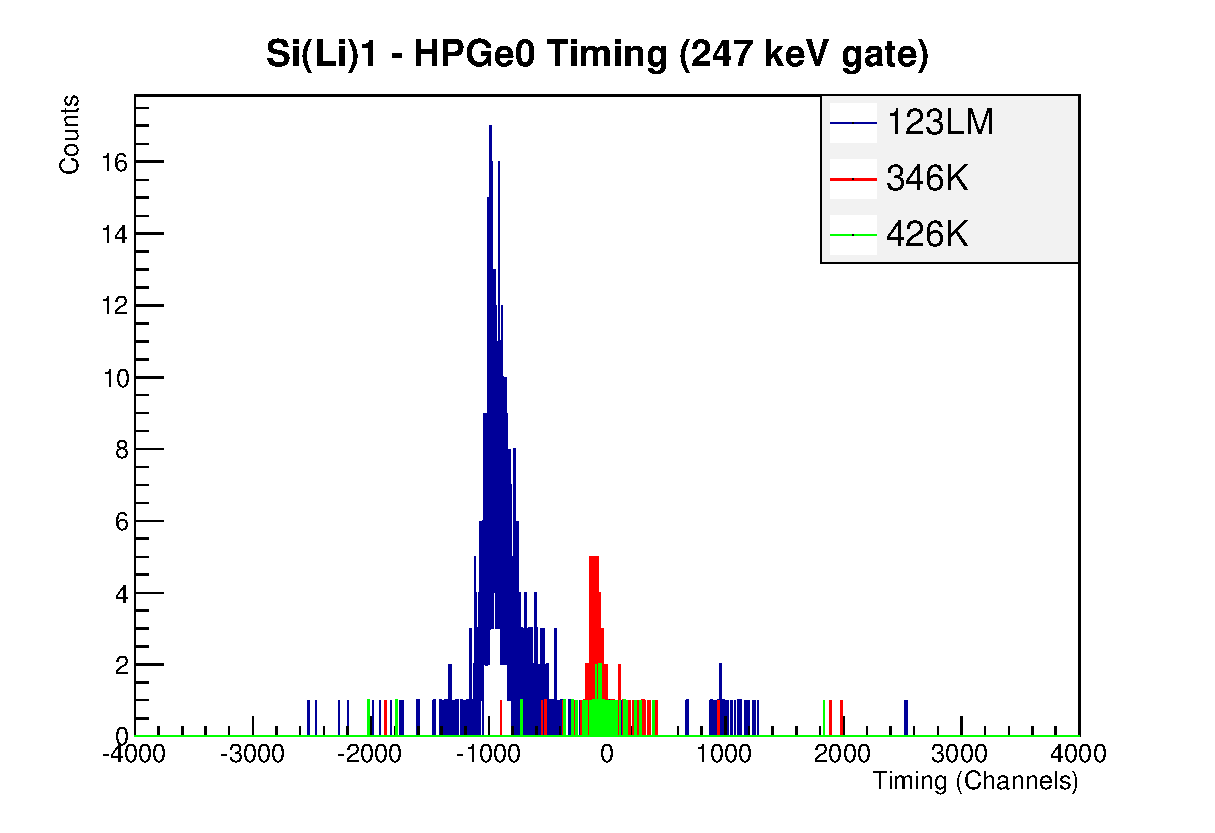
\includegraphics[scale=0.7]{Analysis_Figs/TimingvEnergy.eps}
    \caption[Timing example for the GEORGINA setup]{A plot of the energy-gated timing for a HPGe-Si(Li) detector pairing. The HPGe detector was gated at 247.9 keV, one of the ground state band transitions in the $^{145}$Gd nucleus. The conversion electrons for other transitions in the ground state band were gated on in the Si(Li) detector. Plotted here are the time differences between the two detectors when both peaks were seen in the respective detectors. The 123LM peak was used instead of the K peak due to the high threshold of this detector. As can be seen, the timing has an energy dependence. This dependence is most prominent at lower energies.}
    \label{fig:timing_georgina}
\end{figure}

In the Clovershare data, the timing was done within the electronics, leading to an clean structure, seen in Figure \ref{fig:timing_clover}. Although the same code structure was used for the timing, the gates were all the same within the Clovershare data. The main gate used was $\pm0.3(\mu s)$ and the background ranged from 0.3 to 0.9$(\mu s)$, using the same scaling as seen in Figure \ref{fig:timing_clover}.

\begin{figure}
    \centering
    \includegraphics[scale=0.7]{Analysis_Figs/Timing_clover.eps}
    \caption{Timing between two of the Clovershare detectors, with one detector gated on 123 keV, the lowest transition in the ground state band of $^{154}$Gd. In this data, the gates all looked similarly symmetric, and the timing gates did not need to be varied as they had for the GEORGINA set up.}
    \label{fig:timing_clover}
\end{figure}

Background was taken into account via the energy and timing background gates. The energy background ($E_b$) gate would be subtracted off the main energy gate ($E$). These two energy gates were repeated with the main timing($t$), and background timing($t_b$). The resulting $E-E_b$ spectra, one on the main timing gate, and one on the background timing gate, were then also subtracted as $t-t_b$ to remove any random coincidence from the timing gate.

\section{Systematic Effects}

Several systematic effects had to be taken into account at various stages of analysis. Each will be discussed in further detail in this section. At the calibration stage, there are two major corrections in the Clovershare data. The first, as discussed in section \ref{sec:clover_cal}, is due to the integral non-linearities of the electronics. Second, the instability of the Clovershare detectors required a run-by-run calibration correction. 

In the analysis stage, corrections on extracted values needed to be done based on the angular correlations due to the multipolarity of the radiation and the detectors being at different angles relative to each other. Multipole radiation follows an angular distribution based on the kind of radiation, the multipole of the radiation, and the spin and parity of the initial and final states.

\subsection{Electronics-based Integral Non-Linearities}
\label{sec:non-linearity}

There are two kinds of non-linearities from electronics: integral and differential \citep{knoll00:rad_det_meas}. These two non-linearities are interrelated. Integral linearity is most easily seen in the energy calibration. Differential non-linearity can be seen by looking at the count rate with respect to channel number. Generally, the non-linearity can be expressed in calibration by a higher order correction to an otherwise linear calibration. In the GEORGINA detectors, this was the case. In the Clovershare detectors, this was not the case. 

The Pixie-16 MCA used in the Clovershare experiments has non-linearity specifications for 12-bit and 14-bit modes, but not 16-bit, according to the XIA datasheet \citep{xia:_pixie}. These are listed in terms of the difference of the least significant bit (LSB). In an ideal ADC, this number is 0, meaning the difference between two adjacent channels is exactly one LSB. A larger number means the gap is that much greater than one, and a negative number is that much less. When such non-linearities exist, a best case scenario is for the difference to be constant, leading to the polynomial correction. In the case of the Clovershare experiments, the LSB difference between channels does not appear to be constant.

Plotting the residuals of the calibration after doing a linear fit shows what appears to be a sawtooth pattern to the energy points, as seen in Figure \ref{fig:Clover_ene_res}. To fit this sawtooth pattern, it was assumed that the upward slope of the various sections was the same, and the sections were connected via the error function and complimentary error function, to allow for smoothing of the discontinuity. This results in the function
\begin{equation}
    \begin{aligned}
    	E_{res}= m*x+b_1*Erfc\left(\frac{x-f_1}{c}\right)+b_2*Erf\left(\frac{x-f_1}{c}\right)*\\Erfc\left(\frac{x-f_2}{c}\right)+b_3*Erfc\left(\frac{x-f_2}{c}\right)
    \end{aligned}
\end{equation}
where $m$ is the slope, $b_i$ are the various intercepts to shift the correction, $f_i$ is the location of the shift, and $c$ is the curvature of the error function.

\subsection{Run-based Calibration Corrections}

Run-by-run corrections are usually needed when there is drift or instability in the electronics or pre-amplifier. In the Si(Li) and GEORGINA detectors, there was no noticeable drift. The Clovershare data does appear to need a correction for the HPGe detectors. The best way to track these instabilities was to look at known lines in each run, and plot the residuals after calibration, compared to the known value. This can be seen in Figure \ref{fig:clover_run}.  Several well defined peaks were taken in run to define a linear correction for each run. These linear corrections were done on top of the original energy calibration and correction.

\begin{figure}
    \centering
    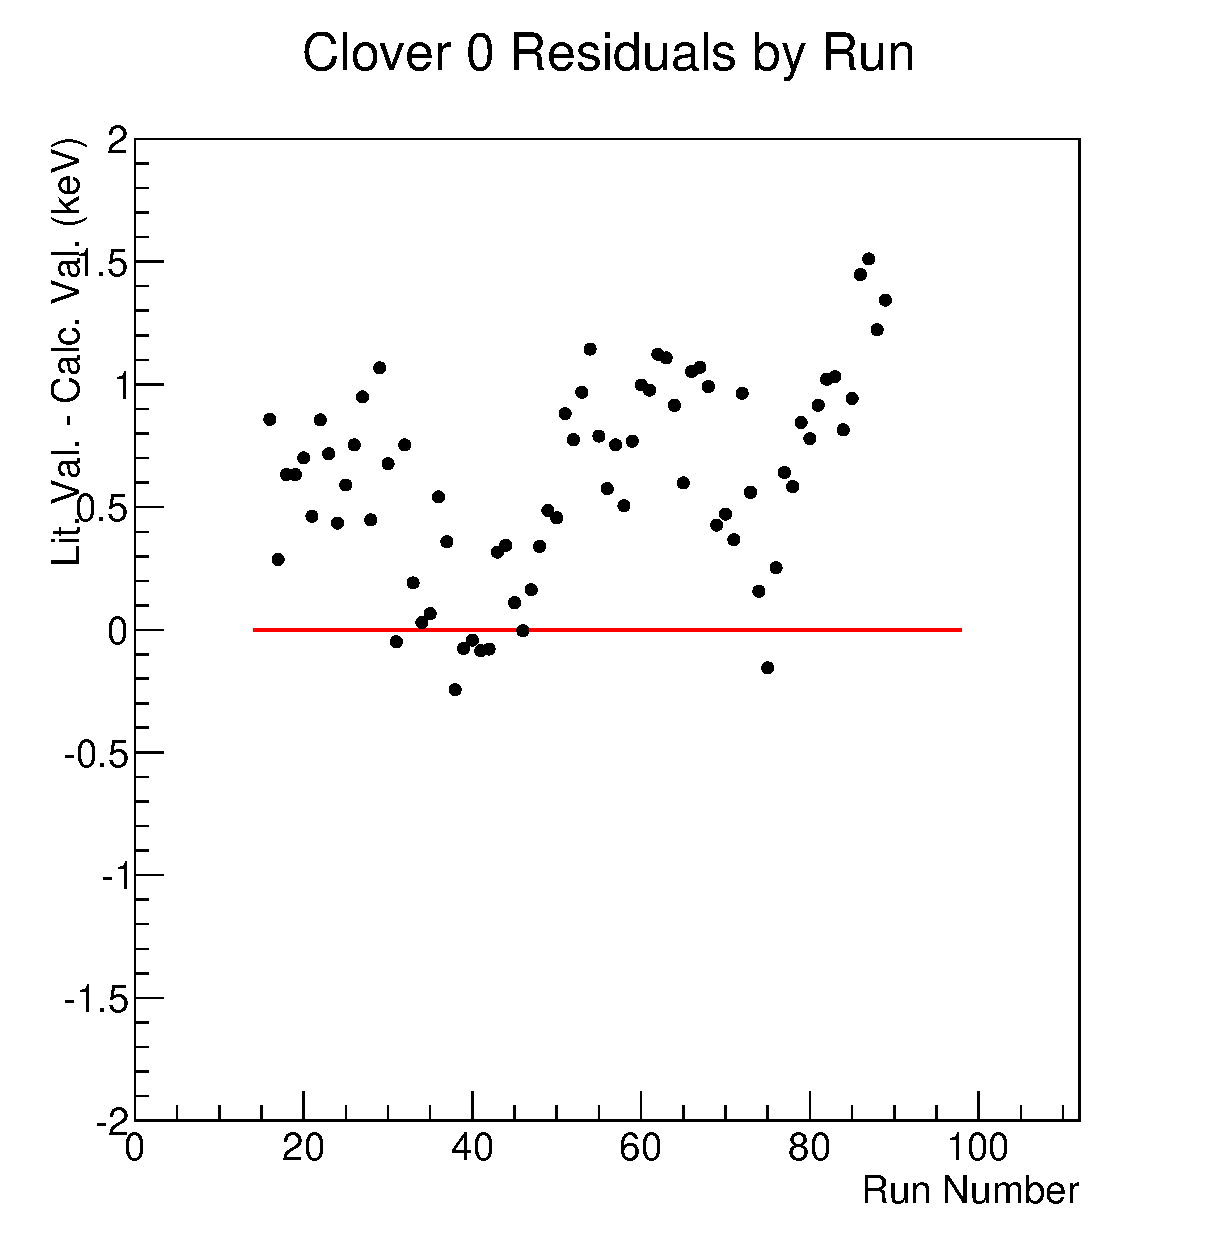
\includegraphics[scale=0.6]{Analysis_Figs/residual_by_run.eps}
    \caption{The difference between the literature value and the calibrated value (before run-by-run correction) of the naturally occurring $^{40}$K background peak at 1460 keV, plotted by run for one leaf of one HPGe detector. The red line shows $\Delta E=0$.}
    \label{fig:clover_run}
\end{figure}

The peaks used for the run-by-run correction were a combination of the ground-state band peaks in the isotope of interest at low energies, and background gammas at higher energies, such as 1460 keV from $^{40}$K and 1764 keV from $^{214}$Bi. These are naturally occurring from the concrete walls of the NSL.

\subsection{Angular Distributions and Angular Correlations}
\label{sec:angular}

Angular correlations are a well studied phenomenon that arises when trying to look at two types of radiation in coincidence. A thorough exploration of different radiation pairings is explored in \citep{biedenharn53:_theory_angular_corr}. For this work, the pairings of interest are $\gamma-\gamma$ and $\gamma-e$. Triple correlations were also explored, as there were several cases where the intermediate transition was not seen. 

Because the detectors are at different angles with respect to each other, when computing conversion coefficients, or subtracting off conversion electrons from the ground state band within the spectra, a correlation must be made based on these relative angles. Table \ref{tab:rel_angle_g} lists these angles from the ICEBall-Georgina setup, with respect to Detector 1. 

These angles can be calculated using
\begin{equation}
    \theta ' = cos^{-1}(\frac{sin\theta_1 cos\phi_1 sin\theta_2 cos\phi_2 +cos\theta_1 cos\phi_1 cos\theta_2 cos\phi_2 + sin\phi_1 sin\phi_2}{\sqrt{2}})
    \label{eq:rel_angle}
\end{equation}
with the previous definitions given for the angles in Tables \ref{tab:ICE_Det_Loc} and \ref{tab:GEORGE_Det_Loc}.

\begin{table}[]
    \centering
    \caption{Relative Angles of Detectors}
    \begin{tabular}{c|c} \toprule
         Detector & $\theta '$  \\
         \hline 
         HPGe 2 & 180 \\
         SiLi 1 & 90\\
         SiLi 2 & 90\\
         SiLi 3 & 122.5\\
         SiLi 4 & 110.7\\
         SiLi 5 & 69.3 \\
         SiLi 6 & 57.3 \\ \bottomrule
    \end{tabular}
    \footnotesize
    \item Relative angles of the detectors with respect to HPGe 1 in the ICEBall-GEORGINA set up. The angles were calculated using Tables \ref{tab:ICE_Det_Loc} and \ref{tab:GEORGE_Det_Loc} and equation \ref{eq:rel_angle}. All angles are in degrees.
    \label{tab:rel_angle_g}
\end{table}

Angular correlation functions for $\gamma-\gamma$ are usually written as a series of Legendre polynomials, multiplied by a correlation coefficient $A_\nu$, or
\begin{equation}
    w(\beta) = \sum_\nu A_\nu P_\nu(cos\beta)
    \label{eq:ge_corr}
\end{equation}
In the case of $\gamma-e$ correlations, the equation becomes 
\begin{equation}
    \begin{split}
        w_m(\beta) = \sum_\nu b_\nu(LLm) A_\nu P_\nu(cos\beta), \\
        w_e(\beta) = \sum_\nu b_\nu(L+1,L+1,e) A_\nu P_\nu(cos\beta)
        \label{eq:e_corr}
    \end{split}
\end{equation}
depending on if the radiation is electric or magnetic in nature. The $b_\nu$ values are based off the same matrix elements used to calculate theoretical conversion coefficients, and are well understood\citep{rose51:_internal_conversion, rose52:_internal_conversion}.

Both of these cases assume pure multipole transitions. In the case of mixed transitions, the correlation function becomes
\begin{equation}
    W = w_I + \delta^2 w_{II} + 2\delta w_{III}
    \label{eq:mixed_corr}
\end{equation}
where $w_I$ and $w_{II}$ are the pure multipole correlation functions, and $w_{III}$ is a correlation mixing the two multipoles. The variable $\delta$ is known as the mixing ratio. 

These correlations can be further extrapolated to look at cases not just of direct correlations, but of indirect correlations, such as three $\gamma$-rays in cascade. If the middle radiation is not observed, the first and third radiations still have a determinable correlation. This is derived for pure multipoles by \citep{biedenharn53:_theory_angular_corr} and for mixed transitions by \citep{rose53:_angular_corr_supp,osborn53:_angular_corr_3}.

For the experiments in this text, the ratios of these angular correlations at the detectors respective angles is needed to adjust for angular effects. Thus, the ratio becomes a factor, $C_{\angle}$, the ratio of the Si(Li) detector angle to the HPGe detector angle with respect to the detector gated on. The conversion coefficient is divided by this factor for correction.

In the singles, a similar value, based on the angular distribution instead of the angular correlation, must be used for correction. Correlations rise out of the angular distribution caused by the multipolarity of different types of radiation, so the angular distribution can also factor into the singles data, with the beam direction acting as the origin angle, making $C_{\angle}$, the ratio of the Si(Li) detector angle to the HPGe detector angle with respect to the beam axis.

The correction must further be adjusted by the solid angle the detector subtends. Only the azimuthal angle of the detector changes the distribution, so integration over slices of the detector with respect to angle can give a weighted average, i.e.
\begin{equation}
    \overline{W}=\frac{1}{\pi r^2}\int^{tan^{-1}(r/d)}_{-tan^{-1}(r/d)}W(\eta+\omega)\left[2\sqrt{r^2-\left(d\times tan(\omega)\right)^2}\right]\frac{d\delta\omega}{cos^2(\omega)}
\end{equation}
where $W(\theta)$ is the angular distribution function, $\eta$ is the azimuthal angle center of the detector, $d$ is the distance of the detector from the target, and $r$ is the radius of the detector, in the same units as $d$. For the Si(Li) detectors, these distances were taken as the maximal coverage of the mini-orange filters, and the distance between the target and the center of the blocker.  Compared to treating the detectors as points, the effects were small, but the solid angle values were used in the singles.

\section{Upper Limits}
\label{sec:upper_limit}

In $^{156}$Gd, there were several possible transitions of interest at energies less than 250 keV. In that energy range, the ground-state band transitions cover much of the spectrum. Some transitions could be removed through the use of gating on gamma-rays of parallel transitions, but not all the transitions could be removed. This was due, in part, to the gate transitions being in sequence with some of the ground-state band. 

To get an upper limit for the transitions of interest, the ground state band transitions that were in sequence with the gate transition were subtracted from of the conversion electron spectrum through the following method. An example of this subtraction can be seen in Figure \ref{fig:subtraction}. The skewed gaussian fitting function described earlier was given parameters derived from the data and subtracted from the conversion electron spectrum.

\begin{figure}
    \centering
    \includegraphics[scale=0.4]{Analysis_Figs/Subtraction_SiLiAll_960.png}
    \caption{An example of the subtraction used to removed the ground state band peaks from spectra. To subtract the conversion electron peak off, the area of the corresponding gamma peak was taken from the same gate. Using the conversion coefficient and the efficiencies of both detectors, the area of the peak could be calculated. From there, this value, along with fixed $R$, $\beta$, $\sigma$, and centroid were used to subtract the peak off. The black line is the function used for subtraction. The blue line is the original spectrum, and the red line is after subtraction. This code can be found in Appendix \ref{chap:macro}}
    \label{fig:subtraction}
\end{figure}

The area of the skewed gaussian is obtained by getting the area of the gamma peak, and adjusting by several factors: efficiencies ($\epsilon$), conversion coefficient ($\alpha$, as derived from theory), and correlation coefficients ($W$). This gives the following:
\begin{equation}
    A_{ce} = A_{\gamma}\times\frac{\epsilon_{ce}}{\epsilon_{\gamma}}\times\alpha\times\frac{W_{ce}}{W_{\gamma}}.
    \label{eq:subt_area_skew}
\end{equation}
The height of the skewed gaussian can be derived in terms of the area, $R$, $\sigma$ and $\beta$ to be
\begin{equation}
    H = A\frac{100}{2*e^{-\frac{\sigma^2}{2\beta^2}}R\sigma-\sqrt{2\pi}(R-100)\sigma};
    \label{eq:subt_height_skew}
\end{equation}
These three variables are all unique to the detector, and come directly from fitting the calibration data, as previously discussed. From there, the parameters can be fed into the equation, along with the centroid of the peak, and subtracted directly off the spectrum. Any remaining counts are counted by taking sections on either side of the area of interest and using a global linear fit for the background, as seen in Figure \ref{fig:piecewise}. This linear fit is subtracted off bin-by-bin in the region of interest. The remaining area is then taken as an upper limit on the transition of interest.

\begin{figure}
    \centering
    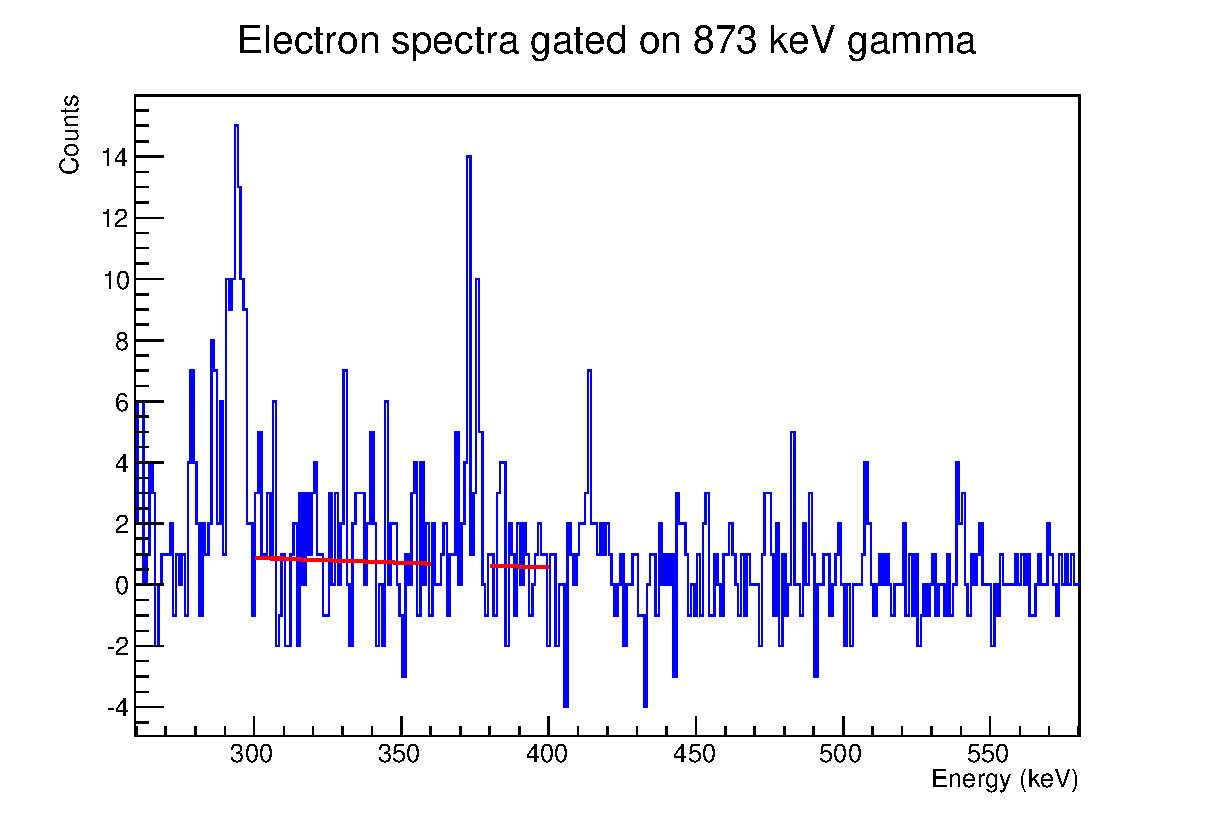
\includegraphics[scale=0.6]{Analysis_Figs/Piecewise_example.eps}
    \caption[An example of the global background fit used for peaks that could not be fit using the skewed gaussian function.]{An example of the global background fit used for peaks that could not be fit using the skewed gaussian function. The areas on either side of the peak are selected by the user. Once the background fit is done, the central area between the two sections is treated as the peak and the background is subtracted off to give a peak area. The red line shows the fit for the background area, and the two sections used for the background fit. See \ref{chap:macro} for the global-fit function used.}
    \label{fig:piecewise}
\end{figure}

\section{Error Analysis}

When areas of peaks were found, the error is found with the fit. In the cases of the peaks that needed to be fit by estimating the background and subtracting it off, the error of the area is assumed to be the square root of the counts in the peak added in quadrature with the error in the background.

These areas are propagated via the equation
\begin{equation}
    \sigma_{f}^2=\sum_{i}\left(\sigma_{x_i}\frac{\delta f}{\delta_{x_i}}\right)^2
\end{equation}
where $f$ is a function of all $x_i$ in the sum \citep{bevington03:_error}. If the function is related to all variables via some form of a polynomial, i.e. $(x_i)^a$ where $a$ is a constant, then it can be rewritten as
\begin{equation}
    \sigma_{f}^2=f*\sum_{i}\left(\frac{\sigma_{x_i}}{a*x_i}\right)^2
\end{equation}
Errors on the areas of both gamma-rays and electrons were propagated through the data. The error on the efficiency was estimated by shifting the efficiency value $\pm0.5\sigma$ and calculating upper and lower limit functions for the efficiency. 

In the final results, the uncertainties were kept separate into statistical and systematic effects. Statistical uncertainties are caused by the areas of the peaks. Systematic effects are from the uncertainty in the efficiency of both the HPGe and Si(Li) detectors, as well as an uncertainty in the angular correlations, based on the solid angle covered by the detectors.

%
% Chapter 4
%

\chapter{$^{154}$Gd Results and Discussion}

\section{Ground State Band Confirmation}
\label{sec:154GS_Confirm}

The first lines looked at in the data are the ground state band of $^{154}$Gd. These lines are all pure E2 transitions, making them an excellent diagnostic to compare with theoretical conversion coefficients. The transitions up to the $10^+$ are summarized and compared with theory in Table \ref{tab:154Gd_Single_ICC_GS}.

For the $6^+\rightarrow 4^+$ and $8^+\rightarrow 6^+$ transitions, electron contributions from smaller gamma lines of similar energy had to be subtracted. This was determined by looking at the conversion coefficients of these transitions in gated spectra, as discussed in the next section. In the gated spectra, the internal conversion coefficients were in agreement with theory, meaning the transitions did not have contaminants. To do so, the gamma-ray had been seen and identified with known multipolarity. The conversion coefficient was then assumed from theory, and the contribution to the area was calculated to be

\begin{equation}
    \label{eq:ICC_Subtract}
    A_{e} = \alpha \epsilon_{e} \frac{A_{\gamma}}{\epsilon_{\gamma}} C_{\angle}
\end{equation}

where $\epsilon_{i}$ are the efficiencies of the electrons and gammas. $C_{\angle}$ is the angular correction for this particular transition. Here, it is multiplied, and not divided, so it can be subtracted from the uncorrected area.

The calculated contributions were subtracted off the fitted area of the electron peak, before the conversion coefficient was calculated. This made the error also include contributions from the errors of these gamma peaks and the errors on the theoretical $\alpha$ values. 

There were two types of transitions that acted as contaminants: those of similar energy, and higher energies whose K-electron energies were similar to the L and M peaks of the lines of interest. The peaks are summarized in Table \ref{tab:154Gd_Contaminants}.

\afterpage{\clearpage\begin{landscape}
    \begin{ThreePartTable}
    \begin{TableNotes}[para,flushleft]
        {\fontsize{10}{12}Table \ref{tab:154Gd_Single_ICC_GS}: A list of ground state band conversion coefficients from $^{154}$Gd. Multipolarities and mixing ratios were taken from the data sheets\citep{reich09:_nds_154}. Unless otherwise stated, the $\alpha$ values are $\alpha_K$. An angular distribution correction has been applied based on multipolarities for pure transitions, and those with known mixing ratios. The first error is statistical, the second is systematic. Numbers are compared with Spits et al.\citep{spits96:_154gd} and Gono et al.\citep{gono74:_154gd_e0}. The starred value was used as an absolute calibration of the conversion electron detector in the Gono work. The dagger lines had contaminant lines subtracted from the conversion electrons. See the text for more details.}
    \end{TableNotes}
    \begin{longtable}{>{\footnotesize}c|>{\footnotesize}c|>{\footnotesize}c|>{\footnotesize}c|>{\footnotesize}c|>{\footnotesize}c|>{\footnotesize}c|>{\footnotesize}c|>{\footnotesize}c|>{\footnotesize}c|>{\footnotesize}c}
        \caption{{\normalsize$^{154}$Gd Ground State Band Internal Conversion Coefficients from Singles}
        \label{tab:154Gd_Single_ICC_GS}}\\
        \toprule
        $E$ (keV)	&	$J^{\pi}	\rightarrow	J^{\pi}$	&	$E_i$ (keV)	&	$E_f$ (keV)	&	$T_{1/2}$ (fs)	&	Multipolarity & Shell &	$\alpha$ (This Work)				&	$\alpha$  (Theory)\citep{kibedi08:_BRICC}	&	$\alpha$ (Spits)\citep{spits96:_154gd}& $\alpha$ (Gono)\citep{gono74:_154gd_e0}	\\
        \hline
        \endfirsthead
        \caption[]{{\normalsize$^{154}$Gd Ground State Band Internal Conversion Coefficients from Singles}}\\
        \toprule
        $E$ (keV)	&	$J^{\pi}	\rightarrow	J^{\pi}$	&	$E_i$ (keV)	&	$E_f$ (keV)	&	$T_{1/2}$ (fs)	&	Multipolarity	& Shell &	$\alpha$ (This Work) &	$\alpha$  (Theory)\citep{kibedi08:_BRICC}	&	$\alpha$ (Spits)\citep{spits96:_154gd}& $\alpha$ (Gono)\citep{gono74:_154gd_e0}		\\
        \hline
	    \endhead
        \endfoot
        \insertTableNotes
        \endlastfoot
	    \hline
        122.23	&	$2^+	\rightarrow	0^+$	&	123.0709	&	0	&	1184000	&	E2	&	K &	0.7759 (34) $^{+148}_{-146}$	&	0.656 (10)	& 0.61 (3) &		\\
    	&				&		&			&		&	& L	&	0.3788 (26) $^{+81}_{-80}$	&	0.411 (6)	&	&	\\
	    &				&		&		&			&	& M	&	0.1323 (3) (29)	&	0.0963 (14)	&	&	\\
	    \hline
        247.85	&	$4^+	\rightarrow	2^+$	&	370.9998	&	123.0709	&	45600	&	E2	&	K &	0.1044	(2) $^{+31}_{-30}$	&	0.1000 (12)	&	0.080 (3)	& 0.0827 (119)\\
	    &				&		&		&		& &	L	&	0.0272	(1) (8)	&	0.0225 (4)	&		\\
	    &				&		&		&		& & M	&	0.0096	(1) (3)	&	0.00513 (8)	&		\\
	    \hline
        346.59$^\dagger$	&	$6^+	\rightarrow	4^+$	&	717.662	&	370.9998	&	8260	&	E2 & K &	0.0335	(1)$^{+11}_{-10}$	&	0.0304 (5)	&	0.029 (1) & 0.0306*	\\
	    &				&		&		&		&	& L	&	0.0087	(1) (3)	&	0.00662 (10)	&		\\
	    &				&		&		&		&	& M	&	0.0027	(1)	(1) &	0.001491 (21)	&		\\
	    \hline
        426.84$^\dagger$	&	$8^+	\rightarrow	6^+$	&	1144.44	&	717.662	&	2570	&	[E2] & K & 0.0180	(2) (5)	&	0.01716 (24)	&	& 0.0170 (22)	\\
    	&				&		&		&		&	& L	&	0.0030	(1) (1)	&	0.00332 (5)	&		\\
	    &				&		&		&		&  	& M	&	0.0008	(1)	(1) &	0.000741 (11)	&		\\
	    \hline
        493.171	&	$10^+	\rightarrow	8^+$	&	1637.05	&	1144.44	&	1110	&	E2	& K	&	0.0124	(4) (4)	&	0.01179 (17)	& &	0.0124 (21)	\\
	    &				&		&		&		&	& L	&	0.0067	(4) (2)	&	0.00213 (3)	&		\\
        \bottomrule
    \end{longtable}
\end{ThreePartTable}
\end{landscape}}

\afterpage{\clearpage\begin{table}[!]
    \centering
    \begin{longtable}{c|c|c|c|c|c|c|c}
        \caption{$^{154}$Gd Ground State Band $6^+\rightarrow 4^+$ and $8^+\rightarrow 6^+$ Electron Peak Contaminants in Singles}
        \label{tab:154Gd_Contaminants} \\
        \toprule
         $E$ & $E_i$ & $E_f$ & $J_i\rightarrow J_f$ & Multipolarity & $\delta$ & Shell & $\alpha$  \\ \hline
         \endhead
         \multicolumn{8}{l}{346.59 keV, $6^+\rightarrow 4^+$} \\ \hline
         338.28 & 1770 & 1432 & $5^+\rightarrow 5^+$ & E0,E2,M1 & -0.004 & K & 0.10 (1) \\ 
         & & & & & $\frac{K(E0)}{K(E2)}\approx 1.0$ & L & 0.01210 (12) \\ 
         & & & & & & M & 0.00180 (3) \\ \hline
         342.18 & 2254 & 1811 & $8^+\rightarrow 6^+$ & E2 & & K & 0.0315 (5) \\ 
         & & & & & & L & 0.0069 (1) \\\
         & & & & & & M & 0.001554 (22) \\ \hline
         390.73 & 1756 & 1366 & $8^+\rightarrow 6^+$ & E2 & & K & 0.0218 (3) \\ \hline
         \multicolumn{8}{l}{426.84 keV, $8^+\rightarrow 6^+$} \\ \hline
         422.12 & 1418 & 996 & $2^+\rightarrow 2^+$ & E0,E2,M1 & Assumed $\approx 1$ & K & 0.114 (16) \\ 
         & & & & & & L & 0.0161 (23) \\ 
         & & & & & & M & 0.0049 (12) \\ \hline
         466.99 & 1719 & 1251 & $2^-\rightarrow 3^-$ & M1,E2 & Assumed $\approx 1$ & K & 0.019 (6) \\ \hline
         479.46 & 1756 & 1366 & $2^-\rightarrow 1^-$ & E2 & & K & 0.01272 (18) \\
         \bottomrule
    \end{longtable}
    \item{A list of the transitions in the $^{154}$Gd Singles data that were contributing to the electron peaks being used for the ground state band lines.}
\end{table}}


\section{Gates on the Ground State Band}
\label{sec:154GS_Gates}

The transitions of the ground state band were the most prominent seen in the gamma-ray and conversion electron spectra. To build a level scheme based on known levels and transitions, these transitions were gated on. Figures \ref{fig:154_2to0}, \ref{fig:154_4to2}, \ref{fig:154_6to4}, and \ref{fig:154_8to6} are the result of these gates. In the cases of cascades, secondary gates were done to confirm assignments.

Determining which transitions went uniquely into a given level was done by comparing the outgoing ground state transition for that level with the incoming transition (i.e. for the $2^+$ level, the 123 keV gate was compared directly with the 247 keV gate). Lines in the gamma spectrum that were present only in the outgoing spectrum, but not the incoming, were assumed to be populating that level.

There were nine bands seen in the gating outside of the ground state band, 4 of which are bands with excited $0^+$ band heads. These are seen in both the $2^+\rightarrow0^+$ gate (Figure \ref{fig:154_2to0}. Three of these bands are seen in the $4^+\rightarrow2^+$ gate (Figure \ref{fig:154_4to2}, and two are seen in the $6^+\rightarrow4^+$ gate (Figure \ref{fig:154_6to4}. Only one is seen in the $8^+\rightarrow6^+$ gate (Figure \ref{fig:154_8to6}. This drop off is not surprising for several reasons, including the lack of known higher spin states in the higher energy $0^+$ bands. The other large reason is the drop off in populating higher energy states in the nucleus.

\begin{figure}[!]
    \centering
    \includegraphics[scale=0.18]{154GdTablesAndFigs/154Gd_2to0.png}
    \caption{Level Scheme of $^{154}$Gd. The gamma ray of the $2^+$\rightarrow$0^+$ transition in the ground state was gated on. It was then compared with the gated spectrum from the gamma ray of the $4^+$\rightarrow$2^+$ transition in the ground state. Peaks only appearing in the first gate were assumed to go into the $2^+$ state, and assignments were made. Due to the low energy of the $2^+$\rightarrow$0^+$ transition, the efficiency was lower, and it is likely that transitions into the $2^+$ state were missed. The levels are organized by band. The lower levels of the band, unseen by gamma rays in this gate, are in gray.}
    \label{fig:154_2to0}
\end{figure}

\begin{figure}[!]
    \centering
    \includegraphics[scale=0.18]{154GdTablesAndFigs/154Gd_4to2.png}
    \caption{Level Scheme of $^{154}$Gd. The gamma ray of the $4^+$\rightarrow$2^+$ transition in the ground state was gated on. It was then compared with the gated spectrum from the gamma ray of the $6^+$\rightarrow$4^+$ transition in the ground state. Peaks only appearing in the first gate were assumed to go into the $4^+$ state, and assignments were made. Additionally, these peaks were also gated on, to look for cascades leading into the $4^+$ state, which were found in several cases. The levels are organized by band. The lower levels of the band, unseen by gamma rays in this gate, are in gray.}
    \label{fig:154_4to2}
\end{figure}

\begin{figure}
    \centering
    \includegraphics[scale=0.2]{154GdTablesAndFigs/154Gd_6to4.png}
    \caption{Level Scheme of $^{154}$Gd. The gamma ray of the $6^+$\rightarrow$4^+$ transition in the ground state was gated on. It was then compared with the gated spectrum from the gamma ray of the $8^+$\rightarrow$6^+$ transition in the ground state. Peaks only appearing in the first gate were assumed to go into the $6^+$ state, and assignments were made. Additionally, these peaks were also gated on, to look for cascades leading into the $6^+$ state, which were found in several cases. The levels are organized by band. The lower levels of the band, unseen by gamma rays in this gate, are in gray.}
    \label{fig:154_6to4}
\end{figure}

\begin{figure}[!]
    \centering
    \includegraphics[scale=0.25]{154GdTablesAndFigs/154Gd_8to6.png}
    \caption{Level Scheme of $^{154}$Gd. The gamma ray of the $8^+$\rightarrow$6^+$ transition in the ground state was gated on. It was then compared with the gated spectrum from the gamma ray of the $10^+$\rightarrow$8^+$ transition in the ground state. Peaks only appearing in the first gate were assumed to go into the $8^+$ state, and assignments were made. Additionally, these peaks were also gated on, to look for cascades leading into the $8^+$ state, which were found in several cases. The levels are organized by band. The lower levels of the band, unseen by gamma rays in this gate, are in gray.}
    \label{fig:154_8to6}
\end{figure}

\section{Conversion Coefficients from Singles}
\label{sec:154_Conv_Singles}

\afterpage{\clearpage\begin{table}
    \centering
    \caption{$^{154}$Gd Internal Conversion Coefficients from Singles}
    \label{tab:154Gd_Single_ICC}
\begin{ThreePartTable}
    \begin{tabular}{c|c|c|c|c|c|c}
        \multicolumn{7}{>{\fontsize{12}{15}}c}{(a)}\\
        \toprule
        $E$ (keV)	&	$J^{\pi}	\rightarrow	J^{\pi}$	&	$E_i$ (keV)	&	$E_f$ (keV)	&	$T_{1/2}$ (fs)	&	Multipolarity	&	$\delta$\\
        \hline
        232.44	&	$4^+_{0^+_2}	\rightarrow	2^+_{0^+_2}$	&	1047.592	&	815.4917	&	7600	&	E2	&	\\
	    &				&		&		&		&		& \\
	    \hline
        329.49	&	$4^+_{0^+_2}	\rightarrow	6^+_{gs}$	&	1047.592	&	717.662	&	7600	&	E2	&	\\
        \hline
        349.89	&	$2^+_{2^+_2}	\rightarrow	0^+_{gs}$	&	1531.305	&	1182.091	&		&	[E2]	&	 \\
        \hline
        416.79	&	$4^+_{0^+_6}	\rightarrow	3^+_{2^+_2}$	&	2080.23	&	1660.903	&		&	(M1)	&	\\
        \hline
        444.19	&	$2^+_{0^+_2}	\rightarrow	4^+_{\gamma}$	&	815.4917	&	370.9998	&	6400	&	E2	&		\\
        \hline
        506.41	&	$5^+_{4^+_1}	\rightarrow	4^+_{\gamma}$	&	1770.187	&	1263.778	&		&	E2	&		\\
        \hline
        515.92	&	$4^+_{4^+_1}	\rightarrow	3^+_{\gamma}$	&	1645.814	&	1127.802	&		&	E2+M1	&	-7 (3)	\\
        \hline
        557.58	&	$0^+_{0^+_2}	\rightarrow	2^+_{gs}$	&	680.6673	&	123.0709	&	4560	&	E2	&		\\
        \hline
        610.71	&	$8^+_{0^+_2}	\rightarrow	8^+_{gs}$	&	1756.49	&	1144.44	&		&	E0+M1+E2	&	-0.69 (14)	\\
	    &				&		&		&		&		&	\\
	    \hline
        676.70	&	$4^+_{0^+_2}	\rightarrow	4^+_{gs}$	&	1047.592	&	370.9998	&	7600	&	E0+M1+E2	&	+2.9 (4)	\\
        \hline
        693.47	&	$2^+_{0^+_2}	\rightarrow	2^+_{gs}$	&	815.4917	&	123.0709	&	6400	&	E2+M1+E0	&	7.5 (4)	\\
        \hline
        873.54	&	$2^+_{\gamma}	\rightarrow	2^+_{gs}$	&	996.2568	&	123.0709	&	950	&	E2+M1+E0	&	-9.4 (4)	\\
        \hline
        889.61	&	$6^+_{\gamma}	\rightarrow	6^+_{gs}$	&	1606.55	&	717.662	&		&	E2+M1	&	$>1.8$	\\
        \hline
        894.40	&	$4^+_{\gamma}	\rightarrow	4^+_{gs}$	&	1263.778	&	370.9998	&		&	E0+M1+E2	&	-3.8 (3)	\\
        \hline
        924.85	&	$4^+_{0^+_2}	\rightarrow	2^+_{gs}$	&	1047.592	&	123.0709	&	7600	&	E2	&	\\
        \hline
        996.33	&	$2^+_{\gamma}	\rightarrow	0^+_{gs}$	&	996.2568	&	0	&	950	&	E2	&	\\
        \hline
        1005.12	&	$3^+_{\gamma}	\rightarrow	2^+_{gs}$	&	1127.8018	&	123.0709	&		&	E2+M1	&	-7.4 (4) \\
        \bottomrule
    \end{tabular}
    \end{ThreePartTable}
\end{table}
\begin{table}
    \begin{ThreePartTable}
        \begin{tabular}{c|c|c|c|c|c}
            \multicolumn{6}{>{\fontsize{12}{15}}c}{TABLE 4.3 (CONTINUED)}\\
            \multicolumn{6}{>{\fontsize{12}{15}}c}{(b)}\\
            \toprule
            $E$ (keV) & Shell &	$\alpha$ (This Work)	&	$\alpha$  (Th)\citep{kibedi08:_BRICC}	&	$\alpha$ (Spits)\citep{spits96:_154gd} & $\alpha$ (Gono)\citep{gono74:_154gd_e0}		\\
            \hline
            232.44	& K &	0.287	(103) $^{+83}_{-82}$	&	0.0982 (14)	&	0.100 (8)	\\
            &	LM &		0.0450	(46) (13)	&	0.0288 (4)	&		\\
            \hline
            329.49	 & K &	0.1573	(89) (17)	&	0.0352 (5)	&	0.034 (3)	\\
            \hline
            349.89	& K &	0.0298 (8) $^{+8}_{-7}$	&	0.0296 (5)	& $<0.097$ &		\\
            \hline
            416.79	 & K &	0.0334	(47) (6)	&	0.03442 (5)	&	\\
            \hline
            444.19	& K &	0.0525	(32) (6)	&	0.01543 (22)	&	0.014 (1)	\\
            \hline
            506.41	& K &	0.0071	(4) (1)	&	0.01098 (16)	&	0.0100 (11)	\\
            \hline
            515.92	& K & 	0.0069	(5) (1)	&	0.0107 (4)	&	0.0113 (9)	\\
            \hline
            557.58	& K &	0.0486	(42) (6)	&	0.00864 (12)	&	0.009 (1) & 0.0091 (16)	\\
            \hline
            610.71	& K &	0.0258	(10) (7)	&	0.0110 (6)	& &	0.053 (7)	\\
            		& L &	0.0167	(9) (4)	&	0.00158 (7)	&		\\
            \hline
            676.70	& K &	0.0283	(4) (10)	&	0.00593 (17)	&	0.0460 (46) & 0.040 (7)	\\
            \hline
            693.47	& K &	0.0017	(2) (1)	&	0.00522 (8)	&	0.0421 (4)	\\
            \hline
            873.54	& K &	0.0021	(3)	(1) &	0.00311 (5)	&	0.0035 (1)	\\
            \hline
            889.61	& K &	0.0043	(6) (2)	&	0.00349 (5)	&	0.0033 (2)	\\
            \hline
            894.40	& K &	0.0019	(2) (1)	&	0.00307 (5)	&	0.0039 (3)	\\
            \hline
            924.85	& K &	0.0033	(9) (1)	&	0.00273 (4)	&	0.0031 (1)	\\
            \hline
            996.33	& K &	0.0021	(4) (1)	&	0.00234 (4)	&	0.0025 (1)	\\
            \hline
            1005.12	& K &	0.0019	(1) (1)	&	0.00233 (4)	&	0.0024 (1)	\\
            \bottomrule
        \end{tabular}
        \begin{tablenotes}[para]
            Table \ref{tab:154Gd_Single_ICC}: A list of conversion coefficients from $^{154}$Gd. Table (a) lists transition information. Multipolarities and mixing ratios were taken from the nuclear data sheets\citep{reich09:_nds_154}. Table (b) lists the conversion coefficients. Unless otherwise stated, the $\alpha$ values are $\alpha_K$. An angular distribution correction has been applied based on multipolarities for pure transitions, and those with known mixing ratios. The first error is statistical, the second is systematic. Numbers are compared with Spits et al.\citep{spits96:_154gd} and Gono et al.\citep{gono74:_154gd_e0} The starred value was used as an absolute calibration of the conversion electron detector in the Gono work. The bands for each level are listed as subscripts.
        \end{tablenotes}
\end{ThreePartTable}
\end{table}
}

\afterpage{\clearpage\begin{landscape}
    \centering
    \begin{table}
    \centering
    \caption{Uncorrected $^{154}$Gd Internal Conversion Coefficients from Singles}
        \label{tab:154Gd_Single_ICC_Uncorr}
\begin{ThreePartTable}
\centering
    \begin{tabular}{>{\footnotesize}c|>{\footnotesize}c|>{\footnotesize}c|>{\footnotesize}c|>{\footnotesize}c|>{\footnotesize}c}
        \multicolumn{6}{>{\fontsize{12}{15}}c}{(a)}\\
        \toprule
        $E$ (keV)	&	$J^{\pi}	\rightarrow	J^{\pi}$	&	$E_i$ (keV)	&	$E_f$ (keV)	&	Multipolarity	&	$\delta$ \\
	    \hline
        198.311	&	$3^-_{1^-}	\rightarrow	2^+_{0^+_3}$	&	1617.123	&	1418.16		&	[E1]	&		\\
        &	$(9)^+_{4^+_1}	\rightarrow	(8)^+_{4^+_1}$	&	2453.29	&	2254.12		&		&	\\
	    \hline
        313.21	&	$3^+_{\gamma}	\rightarrow	2^+_{0^+_2}$	&	1127.802	&	815.492		&	[M1,E2]	&	 \\
        \hline
        641.92	&	$5^+_{4^+_1}	\rightarrow	3^+_{\gamma}$	&	1770.187	&	1127.8018		&	M1,E2	&		\\
        648.951	&	$6^+_{0^+_2}	\rightarrow	6^+_{gs}$	&	1365.87	&	717.662		&	E0+M1+E2	&	+1.30 (20)	\\
        \hline
        715.198	&	$2^+_{2^+_2}	\rightarrow	2^+_{0^+_2}$	&	1531.305	&	815.492		&	E0+M1+E2	&		\\
	    \hline
        1061.59	&	$0^+_{0^+_3}	\rightarrow	2^+_{gs}$	&	1182.091	&	123.0709		&	E2	&		\\
	    &	$5^+_{\gamma}	\rightarrow	4^+_{gs}$	&	1432.588	&	370.9998		&	E2+M1	&	$-4.3^{+12}_{-26}$	\\
        \bottomrule
    \end{tabular}
\end{ThreePartTable}
\end{table}
\end{landscape}
\begin{landscape}
\begin{table}
    \centering
\begin{ThreePartTable}
\centering
    \begin{tabular}{>{\footnotesize}c|>{\footnotesize}c|>{\footnotesize}c|>{\footnotesize}c|>{\footnotesize}c|>{\footnotesize}c|>{\footnotesize}c}
        \multicolumn{7}{>{\fontsize{12}{15}}c}{TABLE 4.4 (CONTINUED)}\\
        \multicolumn{7}{>{\fontsize{12}{15}}c}{(b)}\\
        \toprule
        &  & \multicolumn{2}{>{\footnotesize}c|}{$\alpha$ (This Work)} & & \\
        $E$ (keV)	& Shell	&	Uncorrected & Corrected &	$\alpha$  (Theory)\citep{kibedi08:_BRICC}	&	$\alpha$ (Spits)\citep{spits96:_154gd} & 	$\alpha$ (Gono)\citep{gono74:_154gd_e0}\\
	    \hline
        198.311	& K &	0.0842	(26) (19)	& 0.0568 (18) (13) & 	0.0393 (6)	&		\\
        &	 & 			&	[M1] 0.0986 (30) (22)	& [M1] 0.248 (4) &\\
        &	&	&		[E2] 0.1144 (35) (26)	& [E2] 0.1587 (23) & \\
	    \hline
        313.21	&	 K	&	0.0805	(47) (20)	 & [M1] 0.0543 (32) (13) &	[M1] 0.0723 (11)	&		\\
        	&	&	&	[E2] 0.0832 (49) (21) &	[E2] 0.0407 (6)	&		\\
        \hline
        641.92	& K &	0.0303 (7) (8)	&	0.0249 (6) (2)	 & 0.00615 (9)  &	0.0086 (8)	\\
        648.951	&		&	0.0079 (5)	&	0.0082 (5) & 0.0079 (5) &  & 0.039 (7)	\\
        \hline
        715.198	& K &	0.0199	(5) (5)	& [M1] 0.0299 (8) (8)	& [M1] 0.00879 (13) 	&	0.0070 (5)	\\
        &				  &	& [E2] 0.0150 (4) (4)	& [E2] 0.00479 (7)		& \\
        &				 L &	0.0041	(4) (1)	&	[M1] 0.0061 (6) (2)	& & 		\\
        &				&				  	&	[E2] 0.0031 (3) (1)	& & 		\\
	    \hline
        1061.59	& K &	0.0022	(3) (1)	&	0.0046 (6) (2) & 0.0021 (1)	&		\\
	    &				&	0.0021 (1) & 0.0014 (1) & 0.0019 (4) &	\\
        \bottomrule
    \end{tabular}
% \begin{tablenotes}[para,flushleft]
% 	   Table \ref{tab:154Gd_Single_ICC_Uncorr}: A list of conversion coefficients from $^{154}$Gd. Table (a) lists transition information. Multipolarities and mixing ratios were taken from the nuclear data sheets\citep{reich09:_nds_154}. Table (b) lists the conversion coefficients. Unless otherwise stated, the $\alpha$ values are $\alpha_K$. An angular distribution correction has been applied in the second column of this work, with both the pure M1 and E2 coefficients listed in the cases where the transition does not have a mixing ratio. No M1 information is listed for the $5^+_{4^+}	\rightarrow	3^+_{\gamma}$, as that is not a possible transition by selection rules. The theoretical value for the $6^+_{0^+_2}	\rightarrow	6^+_{gs}$ transition assumes no E0 component. None of the above transitions have known half-lives. The first error is statistical, the second is systematic. Numbers are compared with Spits et al.\citep{spits96:_154gd}. The bands for each level are listed as subscripts.
%     \end{tablenotes}
\end{ThreePartTable}
\end{table}
\begin{table}
    \begin{ThreePartTable}
\begin{tablenotes}[para,flushleft]
    Table \ref{tab:154Gd_Single_ICC_Uncorr}: A list of conversion coefficients from $^{154}$Gd. Table (a) lists transition information. Multipolarities and mixing ratios were taken from the nuclear data sheets\citep{reich09:_nds_154}. Table (b) lists the conversion coefficients. Unless otherwise stated, the $\alpha$ values are $\alpha_K$. An angular distribution correction has been applied in the second column of this work, with both the pure M1 and E2 coefficients listed in the cases where the transition does not have a mixing ratio. No M1 information is listed for the $5^+_{4^+}	\rightarrow	3^+_{\gamma}$, as that is not a possible transition by selection rules. The theoretical value for the $6^+_{0^+_2}	\rightarrow	6^+_{gs}$ transition assumes no E0 component. None of the above transitions have known half-lives. The first error is statistical, the second is systematic. Numbers are compared with Spits et al.\citep{spits96:_154gd}. The bands for each level are listed as subscripts.
 \end{tablenotes}
\end{ThreePartTable}
\end{table}
\end{landscape}}

\afterpage{\clearpage\begin{landscape}
\begin{table}
    \centering
    \caption{$^{154}$Gd Internal Conversion Electrons without Assigned Multipolarities}
    \label{tab:154Gd_No_Mult_ICC}
\begin{ThreePartTable}
        \centering
    \begin{tabular}{>{\footnotesize}c|>{\footnotesize}c|>{\footnotesize}c|>{\footnotesize}c}
        \multicolumn{4}{>{\fontsize{12}{15}}c}{(a)}\\
        \toprule
        $E$ (keV) & $J_i\rightarrow J_f$	& $E_i$ (keV) 	& $E_f$ (keV) \\
	    \hline
	    266.37	&	$6^+_{4^+_1}	\rightarrow	4^+_{4^+_1}$	&	1911.544	&	1645.814 \\ \hline
	    303.89	&	$(7^+)_{4^+_1}	\rightarrow	5^+_{4^+_1}$	&	2073.30	&	1770.187 \\ \hline
	    318.382	&	$6^+_{0^+_2}	\rightarrow	4^+_{0^+_2}$	&	1365.87	&	1047.592	\\
	    &		&		&		\\  \hline
	    379.55	&	$7^+_{\gamma}	\rightarrow	5^+_{\gamma}$	&	1810.21	&	1432.588 \\ \hline
        433.12	&	$4^+_{0^+_6}	\rightarrow	4^+_{4^+_1}$	&	2080.23	&	1645.814	\\ 
        	&	&	&	\\ \hline
        687.05	&	$(5^-)_{0^-} \rightarrow 6^+_{gs}$		&	1404.16	&	717.662 \\ \hline
        722.64	&	$5^+_{4^+_1}	\rightarrow	4^+_{0^+_2}$	&	1770.187	&	1047.592 \\
        &	&	&	\\ \hline
        1033.91	&	$3^-	\rightarrow	4^+_{0^+_2}$	&	2080.791	&	1047.592 \\
        \bottomrule
    \end{tabular}
\end{ThreePartTable}
\end{table}

\begin{table}
    \centering
\begin{ThreePartTable}
    \centering
    \begin{tabular}{>{\footnotesize}c|>{\footnotesize}c|>{\footnotesize}c|>{\footnotesize}c|>{\footnotesize}c|>{\footnotesize}c|>{\footnotesize}c|>{\footnotesize}c}
        \multicolumn{7}{>{\fontsize{12}{15}}c}{TABLE 4.5 (CONTINUED)}\\
        \multicolumn{7}{>{\fontsize{12}{15}}c}{(b)}\\
        \toprule
        &	& \multicolumn{2}{>{\footnotesize}c|}{$\alpha$ (This Work) } & \multicolumn{3}{>{\footnotesize}c|}{Theory\citep{kibedi08:_BRICC}}	& 	\\ 
        $E$ (keV)	& Shell & 	Uncorrected & Corrected 	& $\alpha$(M1) & $\alpha$(E2) & $\alpha$(E1) &	$\alpha$ (Spits)\citep{spits96:_154gd}	\\
	    \hline
	    266.37	& K &	0.2074	(74) (50) & 0.1684 (60) (41) &  & 0.0654 (10) & & \\ \hline
	    303.89	& K &	0.1183	(40) $^{+30}_{-29}$  & 0.0954 (32) $^{+24}_{-23}$ & & 0.0444 (7) & & \\ \hline
	    318.382	& K &	0.0736	(18) (18)  & 0.0600 (15) (15) & & 0.0388 (6) & &\\
	    		& L & 	0.0371	(12) (9) & 0.0301 (10) (7)	& & 0.00892 (13) & &	\\  \hline
	    379.55	& K & 	0.1120	(60) (31) & 0.0903 (48) (25)&  & 0.0236 (4) & & \\ \hline
        433.12	& K &	0.0571	(42) (15) & [M1] 0.0777 (57) (20) & 0.0310 (5) & 0.01650 (24) &	& 0.0220 (45)\\ 
        	&	& & [E2] 0.0351 (26) (9) & & &	& \\ \hline
        687.05	& K & 0.3538 (116) (90) & 0.6435 (211) (163)	& & & 0.00203 (3) &\\ \hline
        722.64	& K		&	0.0166	(12) (42) & [M1] 0.0107 (8) (27)	& 0.00856 (12) & 0.00468 (7) & &		\\
        &	& &  [E2] 0.0185 (13) (47) & & &	& \\ \hline
        1033.91	& K	&	0.0015	(4) (1) & 0.0028 (7) (2)	& & & 0.000916 (13) &	\\
        \bottomrule
    \end{tabular}
\begin{tablenotes}[para]
    Table \ref{tab:154Gd_No_Mult_ICC}: A list of conversion coefficients from $^{154}$Gd without known multipolarities. Table (a) lists transition information. Table (b) lists the conversion coefficients and theoretical values. As a result, an angular distribution correction term cannot be applied to compare with theory, except in the case of pure multipoles. None of the above transitions have known half-lives. The first error is statistical, the second is systematic. Numbers are compared with theoretical coefficients for allowed and reasonable polarities, as well as results from Spits et al. \cite{spits96:_154gd} The bands for each level are listed as subscripts. The $3^-$ for $E=1033.91$ keV has no band placement.
    \end{tablenotes}
\end{ThreePartTable}
\end{table}
\end{landscape}}   

\afterpage{\clearpage\begin{landscape}
    \begin{longtable}{c|c|c|c|c|c|c|c}
        \caption{$0^+\rightarrow 0^+$ Transitions in $^{154}$Gd}
        \label{tab:154Gd_0_to_0}\\
        \toprule
        &	& 	&  &	& \multicolumn{2}{c|}{Theory}	& 	\\ 
        $E_i$ (keV)	&	$E_f$ (keV)	& $E$ (keV)	&	Gate &		$\alpha$ (This Work)	& $\alpha$(M1) & $\alpha$(E2) &	$\alpha$ (Spits)	\\
        \hline
        \endfirsthead
        \toprule
        \caption[]{$0^+\rightarrow 0^+$ Transitions in $^{154}$Gd}\\
        &	& 	&  &	& \multicolumn{2}{c|}{Theory}	& 	\\ 
        $E_i$ (keV)	&	$E_f$ (keV)	& $E$ (keV)	&	Gate &		$\alpha$ (This Work)	& $\alpha$(M1) & $\alpha$(E2) &	$\alpha$ (Spits)	\\
        \hline
	    \endhead
	    \endfoot
	    \multicolumn{8}{p{1.2\textwidth}}{Table \ref{tab:154Gd_0_to_0}: A list of conversion coefficients from $^{154}$Gd for $0^+\rightarrow 0^+$ transitions seen in the gated data. All are lower limits. Numbers are compared with Spits et al.\citep{spits96:_154gd} and theoretical coefficients for M1 and E2 transitions. All coefficients are K-electrons.}
	    \endlastfoot
	    1182.091 & 680.6673 &  501.427 & 557.581 & $>0.0283$ & 0.0213 (3) & 0.01126 (16) & $>0.2$ \\\hline
        1573.9 & 680.6673 &  893.9 & 557.581 & $>0.0183$ & 0.00510 (8) & 0.00294 (5) & \\\hline
        1573.9 & 1182.091 &  391.9 &  1059.033 & $>0.0529$ & 0.0402 (6) & 0.0216 (3) & $>0.1$ \\\hline
        1650.3 & 1182.091 &  468.3 &  1059.033 & $>0.0922$ & 0.0254 (4) & 0.01343 (19) & \\\hline
        1650.3 & 680.6673 &  970.3 & 557.581 & $>0.0209$ & 0.00419 (6) & 0.00247 (4) & $>0.027$ \\
        \bottomrule
	\end{longtable}
\end{landscape}}

\afterpage{\clearpage\begin{landscape}
    \begin{longtable}{>{\small}c|>{\small}c|>{\small}c|>{\small}c|>{\small}c|>{\small}c|>{\small}c|>{\small}c|>{\small}c|>{\small}c}
        \caption{$2^+\rightarrow 2^+$ Transitions in $^{154}$Gd}
        \label{tab:154Gd_2_to_2}\\
        \toprule
        &	& & & 	&  &	& \multicolumn{2}{>{\small}c|}{Theory\citep{kibedi08:_BRICC}}	&	\\ 
        $E_i$ (keV)	& Band &	$E_f$ (keV)	& Band & $E$ (keV)	&	Gate &		$\alpha$ (This Work)	& $\alpha$(M1) & $\alpha$(E2) &	$\alpha$ (Spits)\citep{spits96:_154gd}	\\
        \hline
        \endfirsthead
        \caption[]{$2^+\rightarrow 2^+$ Transitions in $^{154}$Gd}\\
        \toprule
        &	& & & 	&  &	& \multicolumn{2}{>{\small}c|}{Theory\citep{kibedi08:_BRICC}}	&	\\ 
        $E_i$ (keV)	&	Band &	$E_f$ (keV)	& Band & $E$ (keV)	&	Gate &		$\alpha$ (This Work)	& $\alpha$(M1) & $\alpha$(E2) &	$\alpha$ (Spits)\citep{spits96:_154gd}	\\
        \hline
	    \endhead
	    \endfoot
	    \multicolumn{10}{p{1.4\textwidth}}{Table \ref{tab:154Gd_2_to_2}: A list of conversion coefficients from $^{154}$Gd for $2^+\rightarrow 2^+$ transitions seen in the gated data. The first error is statistical, the second is systematic. Numbers are compared with theoretical K-shell conversion coefficients for M1 and E2 transitions, as well as results from Spits et al.\citep{spits96:_154gd} All coefficients are K-electrons.}
	    \endlastfoot
        815.4917 & $0^+_2$ & 123.0709 & GS & 692.4205 & 123.0706 &  0.0430 (3) (9) & 0.00952 (14) & 0.00516 (8) &  0.0421 (4)\\ \hline
        996.264 & $\gamma$ & 815.4917 & $0^+_2$ & 180.72 &  692.4205 & $>1.0570$ & 0.320 (5) & 0.210 (3) &  \\
        &  & &  &  & 444.4924 & $>0.9718$ & & &  \\ \hline
        1418.16 & $0^+_3$ & 815.4917 & $0^+_2$ & 602.688 &  692.4205 & $>0.0125$ & 0.01343 (19) & 0.00715 (10) & 0.025 (3)  \\
        &  & &  &  & 444.4924 & $>0.0093$ &  & &\\ \hline
        1418.16 & $0^+_3$ & 996.2568 & $\gamma$ & 421.893 & 873.1834 & $>0.0367$ & 0.0332 (5) & 0.01170 (25) & 0.114 (16) \\
        &  & &  &  & 625.2556 & $>0.0463$ & & & \\ \hline
        1531.305 & $2^+_2$ & 815.4917 & $0^+_2$ & 715.819 &  692.4205 & 0.0146 (40)$^{+43}_{-33}$ & 0.00877 (13) & 0.00478 (7) & 0.0070 (4)  \\
        &  & &  & & 444.4924 & $0.0234 (80) ^{+68}_{-52}$ & & &\\ \hline
        1531.305 & $2^+_2$ & 996.2568 & $\gamma$ & 535.050 & 873.1834 & 0.0204 (70)$^{+54}_{-41}$ & 0.0181 (3) & 0.00956 (14) & 0.093 (11)  \\
        & & & &  & 625.2556 & $>0.0183$ & & & \\ \hline
        1716.050 & $0^+_6$ & 815.4917 & $0^+_2$ & 900.5583 &  692.4205 & $<0.0105$ & 0.00501 (7) & 0.00289 (4) &  \\
        & & &  & & 444.4924 & $<0.0531$ & & &  \\ \hline
        1716.050 & $0^+_6$ & 996.2568 & $\gamma$ & 719.80 & 873.1834 & 0.0113 (46)$^{+33}_{-25}$ & 0.00865 (13) & 0.00472 (7) & \\
        &  & &  &  & 625.2556 & 0.0501 (260)$^{+147}_{-113}$ & & &  \\ \hline
        1775.429 & $0^+_7$ & 815.4917 & $0^+_2$ & 960.05 &  692.4205 & $>0.0221$ & 0.00430 (6) & 0.00253 (4) &  \\
        &  & & &  & 444.4924 & $>0.0231$ & & &  \\ \hline
        1775.429 & $0^+_7$ & 996.2568 & $\gamma$ & 779.165 & 873.1834 & 0.0206 (112)$^{+60}_{-46}$ & 0.00712 (10) & 0.00396 (6) & \\
        &  & &  &  & 625.2556 & 0.0745 (521)$^{+217}_{-165}$	& & & \\
        \bottomrule
    \end{longtable}
\end{landscape}}

\afterpage{\clearpage\begin{landscape}
    \begin{longtable}{>{\footnotesize}c|>{\footnotesize}c|>{\footnotesize}c|>{\footnotesize}c|>{\footnotesize}c|>{\footnotesize}c|>{\footnotesize}c|>{\footnotesize}c|>{\footnotesize}c|>{\footnotesize}c|>{\footnotesize}c}
        \caption{$4^+\rightarrow 4^+$ Transitions in $^{154}$Gd}
        \label{tab:154Gd_4_to_4}\\
        \toprule
        &	& & & 	&  &	& \multicolumn{2}{>{\footnotesize}c|}{Theory\citep{kibedi08:_BRICC}}	& & 	\\ 
        $E_i$ (keV)	& Band &	$E_f$ (keV)	& Band & $E$ (keV)	&	Gate &		$\alpha$ (This Work)	& $\alpha$(M1) & $\alpha$(E2) &	$\alpha$ (Spits)\citep{spits96:_154gd}
        & $\alpha$ (Gono)\citep{gono74:_154gd_e0}	\\
        \hline
        \endfirsthead
        \caption[]{$4^+\rightarrow 4^+$ Transitions in $^{154}$Gd}\\
        \toprule
        &	& & &	&  &	& \multicolumn{2}{>{\footnotesize}c|}{Theory\citep{kibedi08:_BRICC}}	& &	\\ 
        $E_i$ (keV)	& Band &	$E_f$ (keV)	& Band & $E$ (keV)	&	Gate &		$\alpha$ (This Work)	& $\alpha$(M1) & $\alpha$(E2) &	$\alpha$ (Spits)\citep{spits96:_154gd}
        & $\alpha$ (Gono)\citep{gono74:_154gd_e0}	\\
        \hline
	    \endhead
	    \endfoot
	    \multicolumn{11}{p{1.4\textwidth}}{Table \ref{tab:154Gd_4_to_4}: A list of conversion coefficients from $^{154}$Gd for $4^+\rightarrow 4^+$ transitions seen in the gated data. The first error is statistical, the second is systematic. Numbers are compared with theoretical K-shell conversion coefficients for M1 and E2 transitions, as well as results from Spits et al.\citep{spits96:_154gd} and Gono et al.\citep{gono74:_154gd_e0} All coefficients are K-electrons, except for the transition from 1047 keV. The second value is the LM peak.}
	    \endlastfoot
        1047.592 & $0^+_2$ & 370.9998 & GS &  676.593 & 247.9288 & 0.0550 (2)$^{+12}_{-11}$ & 0.01007 (15) & 0.00544 (8) & 0.0460 (46) & 0.040 (7)\\
        &  & & &   &  & 0.0131 (1) (3) & 0.001384 (20) & 0.000870 (13) & & \\ \hline
        1263.778 & $\gamma$ & 1047.592 & $0^+_2$ & 216.186 & 676.593 & $<0.1250$ & 0.196 (3) & 0.1222 (18) &  \\
         & & &   &  & 924.55 & $<0.1033$ & & &  \\ \hline
        1645.814 & $4^+_1$ & 1047.592 & $0^+_2$ & 598.22 & 676.593 &  $<0.0092$ &  0.01368 (20) & 0.00728 (11) & $<0.067$  \\
         & & &   &  & 924.55 &  $<0.0142$ & & & \\ \hline
        1645.814 & $4^+_1$ & 1263.778 & $\gamma$ & 382.025 & 892.775 & $<0.0360$ & 0.0429 (6) & 0.0232 (4) & 0.033 (5) \\
         & & &   &  & 1140.702 & $<0.0494$ & & & \\ \hline
        1701.39 & $0^+_3$ & 1047.592 & $0^+_2$ & 653.7 & 676.593 & $<0.0093$ & 0.01097 (16) & 0.00590 (9) & 0.0220 (62)  \\
        &  & &  &  & 924.55 & $<0.0301$ & & & \\ \hline
        1701.39 & $0^+_3$ & 1263.778 & $\gamma$ & 437.612 & 892.775 & $<0.0585$ & 0.0302 (5) & 0.01605 (23) &   \\
        &  & &  &  & 1140.702 & $<0.0511$ & & &   \\ \hline
        1789.17 & $2^+_2$ & 1047.592 & $0^+_2$ & 740.91 & 676.593 & $<0.0124$ & 0.00806 (12) & 0.00443 (7) & \\
        &  & &  &  & 924.55 & $<0.0447$ & & &  \\ \hline
        1789.17 & $2^+_2$ & 1263.778 & $\gamma$ & 525.392 & 892.775 & $<0.0168$ & 0.0190 (3) & 0.01001 (14) &  \\
        &  & &  &  & 1140.702 & $<0.0161$ & & &  \\
        \bottomrule
    \end{longtable}
\end{landscape}}

\afterpage{\clearpage\begin{sidewaystable}
    \small
    \begin{longtable}{c|c|c|c|c|c|c|c}
        \caption{$6^+\rightarrow 6^+$ Transitions in $^{154}$Gd}
        \label{tab:154Gd_6_to_6}\\
        \toprule
        &	& 	&  &	& \multicolumn{2}{c|}{Theory}	& 	\\ 
        $E_i$ (keV)	&	$E_f$ (keV)	& $E$ (keV)	&	Gate &		$\alpha$ (This Work)	& $\alpha$(M1) & $\alpha$(E2) &	$\alpha$ (Gono)	\\
        \hline
        \endfirsthead
        \toprule
        \caption[]{$6^+\rightarrow 6^+$ Transitions in $^{154}$Gd}\\
        &	& 	&  &	& \multicolumn{2}{c|}{Theory}	& 	\\ 
        $E_i$ (keV)	&	$E_f$ (keV)	& $E$ (keV)	&	Gate &		$\alpha$ (This Work)	& $\alpha$(M1) & $\alpha$(E2) &	$\alpha$ (Gono)	\\
        \hline
    	\endhead
        1365.878 & 717.662 & 648.3 & 346.643 & 0.0778 (4) (16) & 0.01120 (16) & 0.00601 (9) & 0.039 (7)\\ \hline
        1606.55 & 1365.878 & 240.672 & 648.3 & $>0.9065$ & 0.1462 (21) & 0.0885 (13) &  \\
        &  &  & 994.9 & $>1.1070$ & & &  \\ \hline
        1911.544 & 1365.878 & 545.7 & 648.3 &  $<0.0209$ & 0.01723 (25) & 0.00911 (13) &   \\
        &  &  & 994.9 &  $<0.0189$ &  & &  \\ \hline
        1911.544 & 1606.55 & 304.75 & 888.69 & $<0.0794$ & 0.0777 (11) & 0.0440 (7) & 0.042 (6) \\
        \bottomrule
    \end{longtable}
    \item{A list of conversion coefficients from $^{154}$Gd for $6^+\rightarrow 6^+$ transitions seen in the gated data. The first error is statistical, the second is systematic. Numbers are compared with theoretical K-shell conversion coefficients for M1 and E2 transitions, as well as results from Gono et al.\citep{gono74:_154gd_e0} All coefficients are K-electrons.}
\end{sidewaystable}}
    

%
% Chapter 5
%

\chapter{$^{156}$Gd Results and Discussion}

%\section {Oh HAY! FIGURES BIOTCH!}

\begin{figure}
    \centering
    \includegraphics[scale=0.3]{156GdTablesAndFigs/156Gd_2to0.png}
    \caption{Level Scheme of $^{156}$Gd. The gamma ray of the $2^+$\rightarrow$0^+$ transition in the ground state was gated on. It was then compared with the gated spectrum from the gamma ray of the $4^+$\rightarrow$2^+$ transition in the ground state. Peaks only appearing in the first gate were assumed to go into the $2^+$ state, and assignments were made. Due to the low energy of the $2^+$\rightarrow$0^+$ transition, the efficiency was lower, and it is likely that transitions into the $2^+$ state were missed. The levels are organized by band. The lower levels of the band, unseen by gamma rays in this gate, are in gray.}
    \label{fig:156_2to0}
\end{figure}

\begin{figure}
    \centering
    \includegraphics[scale=0.28]{156GdTablesAndFigs/156Gd_4to2.png}
    \caption{Level Scheme of $^{156}$Gd. The gamma ray of the $4^+$\rightarrow$2^+$ transition in the ground state was gated on. It was then compared with the gated spectrum from the gamma ray of the $6^+$\rightarrow$4^+$ transition in the ground state. Peaks only appearing in the first gate were assumed to go into the $4^+$ state, and assignments were made. Additionally, these peaks were also gated on, to look for cascades leading into the $4^+$ state, which were found in several cases. The levels are organized by band. The lower levels of the band, unseen by gamma rays in this gate, are in gray.}
    \label{fig:156_4to2}
\end{figure}

\begin{figure}
    \centering
    \includegraphics[scale=0.28]{156GdTablesAndFigs/156Gd_6to4.png}
    \caption{Level Scheme of $^{156}$Gd. The gamma ray of the $6^+$\rightarrow$4^+$ transition in the ground state was gated on. It was then compared with the gated spectrum from the gamma ray of the $8^+$\rightarrow$6^+$ transition in the ground state. Peaks only appearing in the first gate were assumed to go into the $6^+$ state, and assignments were made. Additionally, these peaks were also gated on, to look for cascades leading into the $6^+$ state, which were found in several cases. The levels are organized by band. The lower levels of the band, unseen by gamma rays in this gate, are in gray.}
    \label{fig:156_6to4}
\end{figure}

\begin{figure}
    \centering
    \includegraphics[scale=0.3]{156GdTablesAndFigs/156Gd_8to6.png}
    \caption{Level Scheme of $^{156}$Gd. The gamma ray of the $8^+$\rightarrow$6^+$ transition in the ground state was gated on. It was then compared with the gated spectrum from the gamma ray of the $10^+$\rightarrow$8^+$ transition in the ground state. Peaks only appearing in the first gate were assumed to go into the $8^+$ state, and assignments were made. Additionally, these peaks were also gated on, to look for cascades leading into the $8^+$ state, which were found in several cases. The levels are organized by band. The lower levels of the band, unseen by gamma rays in this gate, are in gray.}
    \label{fig:156_8to6}
\end{figure}

%\section{LOOK! A TABLE!}

\begin{landscape}
    \begin{longtable}{>{\footnotesize}c|>{\footnotesize}c|>{\footnotesize}c|>{\footnotesize}c|>{\footnotesize}c|>{\footnotesize}c|>{\footnotesize}c|>{\footnotesize}c|>{\footnotesize}c|>{\footnotesize}c}
    \caption{$^{156}$Gd Ground State Band Internal Conversion Coefficients from Singles}
        \label{tab:156Gd_Single_ICC_GS}\\
    \toprule
$E$ (keV)	&	$J^{\pi}	\rightarrow	J^{\pi}$	&	$E_i$ (keV)	&	$E_f$ (keV)	&	$T_{1/2}$ (fs)	&	Multipolarity	&	Shell & $\alpha$ (This Work)	&	$\alpha$  (Th)	&	$\alpha$ (Konijn)	\\
\hline		
\endfirsthead
    \caption[]{$^{156}$Gd Ground State Band Internal Conversion Coefficients from Singles}\\
    \toprule
$E$ (keV)	&	$J^{\pi}	\rightarrow	J^{\pi}$	&	$E_i$ (keV)	&	$E_f$ (keV)	&	$T_{1/2}$ (fs)	&	Multipolarity	&	Shell & $\alpha$ (This Work)	&	$\alpha$  (Th)	&	$\alpha$ (Konijn)	\\
\hline		
\endhead
\endfoot
\multicolumn{10}{p{1.4\textwidth}}{A list of the ground state conversion coefficients from $^{156}$Gd. Multipolarities and mixing ratios were taken from the nuclear data sheets\citep{reich12:_nds_156}. Unless otherwise stated, the $\alpha$ values are $\alpha_K$. An angular distribution correction has been applied based on multipolarities for pure transitions, and those with known mixing ratios. The first error is statistical, the second is systematic. Numbers are compared with Konijn et al. \citep{konijn81:_156gd} Starred values in the Konijn data were used as calibration points.}
\endlastfoot
198.58	&	$4^+	\rightarrow	2^+$	&	288.187	&	88.97	&	111900	&	E2	& K &	0.1667 (4)$^{+46}_{-45}$	&	0.1565 (22)	&	0.199 (36)	\\
	&				&		&		&		&		& L &	0.0537 (1)$^{+16}_{-15}$	&	0.0531 (8)	&		\\
	&			&		&		&		&		& M &	0.0170 (1) (5)	&	0.0122 (2)	&		\\ \hline
296.04	&	$6^+	\rightarrow	4^+$	&	584.715	&	288.187	&	15800	&	E2 & K	&	0.0572 (1) (18)	&	0.0477 (7)	&	0.04683*	\\
	&				&		&		&		&	& L	&	0.0121 (1) (4)	&	0.0115 (2)	&		\\
	&				&		&		&		&	& M	&	0.0036 (1) (1) &	0.0026 (1)	&		\\ \hline
379.92	&	$8^+	\rightarrow	6^+$	&	965.134	&	584.715	&	4320	&	E2 & K	&		0.0274 (1) (9)	&	0.0235 (4)	&	0.038 (10)	\\
	&				&		&		&		&	& L	&	0.0050 (1) (2)	&	0.0048 (1)	&		\\
	&				&		&		&		&	& M	&	0.0013 (1) (1)	&	0.0011 (1)	&		\\ \hline
	\pagebreak
450.64	&	$10^+	\rightarrow	8^+$	&	1416.078	&	965.134	&	1900	&	E2	& K &	0.0152 (2) (5)	&	0.01483 (21)	& 0.0145*		\\
	&				&		&		&		&	& L	&	0.0028 (1) (1)	&	0.00279 (4)	&		\\
	&				&		&		&		&	& M	&	0.0010 (1) (1)	&	0.000621 (9)	&		\\ 
\bottomrule
    \end{longtable}
\end{landscape}

\begin{landscape}
    \begin{longtable}{c|c|c|c|c|c|c|c|c|c|c}
    \caption{$^{156}$Gd Internal Conversion Coefficients from Singles}
        \label{tab:156Gd_Single_ICC_Corr}\\
    \toprule
$E$ (keV)	&	$J^{\pi}	\rightarrow	J^{\pi}$	&	$E_i$ (keV)	&	$E_f$ (keV)	&	$T_{1/2}$ (fs)	&	Multipolarity	&	$\delta$	& Shell &	$\alpha$ (This Work)	&	$\alpha$  (Th)	&	$\alpha$ (Konijn)	\\
\hline		
\endfirsthead
    \caption[]{$^{156}$Gd Internal Conversion Coefficients from Singles}\\
    \toprule
$E$ (keV)	&	$J^{\pi}	\rightarrow	J^{\pi}$	&	$E_i$ (keV)	&	$E_f$ (keV)	&	$T_{1/2}$ (fs)	&	Multipolarity	&	$\delta$ & Shell &	$\alpha$ (This Work)	&	$\alpha$  (Th)	&	$\alpha$ (Konijn)	\\
\hline		
\endhead
227.90	&	$7^-	\rightarrow 7^+$	&	2137.6	&	1909.26	&	1300000000	&	E1	&	& K	&	0.4704 (50)$^{+85}_{-84}$	&	0.0272 (4)	&	0.063 (13)	\\
	&			&		&		&		&		&	& LM	&	0.1077 (20) (20)	&	0.0049 (6)	&		\\ \hline
321.92	&	$8^-	\rightarrow	6^-$	&	2027.1	&	1705.799	&		&	E2	&		& K &	0.0283 (13) (9)	&	0.0378 (6)	&	0.025 (7)	\\ \hline
355.87	&	$4^+	\rightarrow	2^+$	&	1510.594	&	1154.152	&	189000	&	E2	&		& K &	0.0156 (6) (5)	&	0.0281 (4)	&	\\ \hline
399.56	&	$9^+	\rightarrow	7^+$	&	2249.65	&	1849.84	&		&	E2	&		& K &	0.0075 (8) (3)	&	0.0205 (3)	&	0.026 (5)	\\ \hline
921.83	&	$5^+	\rightarrow	6^+$	&	1506.863	&	584.715	&	400	&	E2	&		& K &	0.0043 (9) (5) &	0.0028 (1)	&	0.0030 (7)	\\ \hline
1039.55	&	$5^+	\rightarrow	6^+$	&	1622.39	&	584.715	&		&	E2+M1	&	-7	& K &	0.0152 (10) (2)	&	0.0022 (1)	&	0.0142 (33)	\\ \hline
1059.31	&	$6^+	\rightarrow	6^+$	&	1643.653	&	584.715	&		&	E2	&		& K &	0.0011 (4) (1)	&	0.0021 (1)	&	0.0013 (8)	\\ \bottomrule
    \end{longtable}
    \caption{A list of conversion coefficients from $^{156}$Gd. Multipolarities and mixing ratios were taken from NNDC. Unless otherwise stated, the $\alpha$ values are $\alpha_K$. An angular distribution correction has been applied based on multipolarities for pure transitions, and those with known mixing ratios. The first error is statistical, the second is systematic. Numbers are compared with Konijn et al. \citep{konjin81:_156gd}}
\end{landscape}

\begin{landscape}
    \begin{longtable}{c|c|c|c|c|c|c|c|c|c}
    \caption{Uncorrected $^{156}$Gd Internal Conversion Coefficients from Singles}
        \label{tab:156Gd_Single_ICC_Uncorr}\\
    \toprule
$E$ (keV)	&	$J^{\pi}	\rightarrow	J^{\pi}$	&	$E_i$ (keV)	&	$E_f$ (keV)	&	$T_{1/2}$ (fs)	&	Multipolarity	&	$\delta$	&	$\alpha$ (This Work)	&	$\alpha$  (Th)	&	$\alpha$ (Konijn)	\\
\hline		
\endfirsthead
    \caption[]{Uncorrected $^{156}$Gd Internal Conversion Coefficients from Singles}\\
    \toprule
$E$ (keV)	&	$J^{\pi}	\rightarrow	J^{\pi}$	&	$E_i$ (keV)	&	$E_f$ (keV)	&	$T_{1/2}$ (fs)	&	Multipolarity	&	$\delta$	&	$\alpha$ (This Work)	&	$\alpha$  (Th)	&	$\alpha$ (Konijn)	\\
\hline		
\endhead
154.94	&	$4^+	\rightarrow	4^+$	&	1510.594	&	1355.422	&	189000	&	M1+E2	&	0.48	&	0.4635 (183)$^{+98}_{-97}$	&	0.460 (7)	& \\
	&	$7^+	\rightarrow	6^+$	&	1909.26	&	1753.653	&		&	(M1+E2)	&	0.29	&		&	0.474 (7)	&		\\ \hline
883.86	&	$8^+	\rightarrow	8^+$	&	1848.33	&	965.134	&		&	E0+E2	&		&	0.0057 (7) (1)	&	0.0030 (1)	& $>0.0092$		\\
	&	$7^+	\rightarrow	8^+$	&	1849.84	&	965.134	&		&	E2(+M1)	&		&		&	0.0030 (1)	&	$<0.0052$	\\ \hline
955	&	$6^+	\rightarrow	6^+$	&	1540.19	&	584.715	&		&	E0+E2	&		&	0.0065 (4) (5)	&	0.0026 (1)	&	0.020 (8)	\\ 
959.88	&	$0^+	\rightarrow	2^+$	&	1049.487	&	88.97	&	1800	&	E2	&		&	&	0.0025 (1)	&	0.0045 (24)	\\
	&	$3^+	\rightarrow	4^+$	&	1248.006	&	288.197	&	580	&	E2+M1	&	-12	&		&	0.0025 (1)	&		\\ \hline
1009.33	&	$4^+	\rightarrow	4^+$	&	1297.822	&	288.197	&	1600	&	E0+E2,M1	&		&	0.0173 (9) (4)	&		&	0.0164 (29)	\\ \hline
1045.48	&	$8^+	\rightarrow	8^+$	&	2011.38	&	965.134	&		&	E2(+M1)	&		&	0.0012 (2) (2)	&	0.0021 (1)	&	0.0025 (6)	\\ 
1052.61	&	$7^-	\rightarrow	6^+$	&	1638	&	584.715	&		&	E1	&		&		&	0.0009 (1)	&		\\ \hline
1065.74	&	$2^+	\rightarrow	2^+$	&	1154.152	&	88.97	&	568	&	E2+M1	&	-16	&	0.0023 (2) (1)	&	0.0021 (1)	&	0.0025 (9)	\\
	&	$4^+	\rightarrow	4^+$	&	1355.422	&	288.187	&	540	&	E2+M1	&	-4	&		&	0.0021 (3)	&	0.0021 51)	\\ \hline
1158.65	&	$2^+	\rightarrow	0^+$	&	1154.152	&	0	&	568	&	E2	&		&	0.0020 (3) (1)	&	0.0017 (1)	&	0.0023 (3)	\\
	&	$3^+	\rightarrow	2^+$	&	1248.006	&	88.97	&	580	&	E2+M1	&	-11.8	&		&	0.0017 (1)	&		\\ \hline
1168.69	&	$0^+	\rightarrow	0^+$	&	1168.186	&	0	&	5000	&	E0	&		&	0.0045 (3) (1)	&		&	$>0.0035$	\\
	&	$2^+	\rightarrow	2^+$	&	1258.075	&	88.97	&	1540	&	E2+M1+E0	&	0.38	&		&	0.0026 (1)	&		\\ \hline
1222.22	&	$4^+	\rightarrow	4^+$	&	1510.594	&	288.197	&	189000	&	M1+E2	&	-1.7	&	0.0028 (4) (1)	&	0.0018 (1)	&	0.00174*	\\
	&	$5^+	\rightarrow	4^+$	&	1506.863	&	288.197	&	400	&	E2	&		&		&	0.001560 (22)	&	\\ \hline
1264.85	&	$4^+	\rightarrow	2^+$	&	1355.422	&	88.97	&	540	&	E2	&		&	0.0017 (3) (1)	&	0.0014 (1)	&	\\
	&	$8^+	\rightarrow	6^+$	&	1848.33	&	584.715	&		&		&		&		&		&		\\
	&	$7^+	\rightarrow	6^+$	&	1849.84	&	584.715	&		&		&		&		&		&		\\ \bottomrule
    \end{longtable}
    \caption{A list of conversion coefficients from $^{156}$Gd. Multipolarities and mixing ratios were taken from NNDC. Unless otherwise stated, the $\alpha$ values are $\alpha_K$. No angular distribution correction has been applied, either due to unknown mixing ratios, or multiple assignments of the gamma-ray. The first error is statistical, the second is systematic. Numbers are compared with Konijn et al. \citep{konjin81:_156gd} Starred values were used as calibration points in the Konijn paper. All coefficients are K-shell electrons.}
\end{landscape}

\begin{landscape}
    \begin{longtable}{c|c|c|c|c|c|c|c|c}
        \caption{$^{156}$Gd Internal Conversion Electrons without known Multipolarities}
        \label{tab:156Gd_No_Mult_ICC}\\
        \toprule
        &	& 	&  &	& \multicolumn{3}{c|}{Theory}	& 	\\
        $E_i$ (keV)	&	$E_f$ (keV)	& $E$ (keV)	&	Gate &		$\alpha$ (This Work)	& $\alpha$(M1) & $\alpha$(E2) & $\alpha$(E1) &	$\alpha$ (Konijn)	\\
        \hline		
        \endfirsthead
        \caption[]{$^{156}$Gd Internal Conversion Electrons without known Multipolarities}\\
        \toprule
        &	& 	&  &	& \multicolumn{3}{c|}{Theory}	& 	\\
        $E_i$ (keV)	&	$E_f$ (keV)	& $E$ (keV)	&	Gate &		$\alpha$ (This Work)	& $\alpha$(M1) & $\alpha$(E2) & $\alpha$(E1) &	$\alpha$ (Konijn)	\\
        \hline		
        \endhead
        \endfoot
        \multicolumn{9}{p{1.4\textwidth}}{A list of conversion coefficients from $^{156}$Gd without known multipolarities. As a result, an angular distribution correction term has not been applied. None of the states have known half lives. The first error is statistical, the second is systematic. Numbers are compared with theoretical values for allowed multipolarities and results from Konijn et al. \citep{konijn81:_156gd}. All coefficients are K-shell electrons.}
        \endlastfoot
        671.41	&	$7^-	\rightarrow	8^+$	&	1638	&	965.134	&		0.0064 (6) (2)	& & & 0.00213 (3) &	\\ \hline
        838.83	&	$9^+	\rightarrow	10^+$	&	2249.65	&	1416.078	&	0.0009 (3) (1)	& 0.00595 (9) & 0.00337 (5) & & 	\\ \hline
        943.732	&	$7^+	\rightarrow	8^+$	&	1909.26	&	965.134		&	0.0022 (6) (1) & 0.00448 (7) & 0.00262 (4) & &	0.0025 (3)	\\ 
        \bottomrule
    \end{longtable}
\end{landscape}
    
\begin{landscape}
    \begin{longtable}{c|c|c|c|c|c|c|c}
        \caption{$0^+\rightarrow 0^+$ Transitions in $^{156}$Gd}
        \label{tab:156Gd_0_to_0}\\
        \toprule
        &	& 	&  &	& \multicolumn{2}{c|}{Theory}	& 	\\
        $E_i$ (keV)	&	$E_f$ (keV)	& $E$ (keV)	&	Gate &		$\alpha$ (This Work)	& $\alpha$(M1) & $\alpha$(E2) &	$\alpha$ (Konijn)	\\
        \hline
        \endfirsthead
        \toprule
        \caption[]{$0^+\rightarrow 0^+$ Transitions in $^{156}$Gd}\\
        &	& 	&  &	& \multicolumn{2}{c|}{Theory}	& 	\\
        $E_i$ (keV)	&	$E_f$ (keV)	& $E$ (keV)	&	Gate &		$\alpha$ (This Work)	& $\alpha$(M1) & $\alpha$(E2) &	$\alpha$ (Konijn)	\\
	    \endhead
        1168.186 & 1049.487  & 118.71 &  960.50771 & $>1.1970$ & 1.042 (15) & 0.726 (11) & \\
        \bottomrule
    \end{longtable}
    \caption{A list of conversion coefficients from $^{156}$Gd for $0^+\rightarrow 0^+$ transitions seen in the gated data. All listed theoretical values are for the K-shell internal conversion coefficient. Numbers are compared with theoretical values for allowed multipolarities and results from Konijn et al.\citep{konjin81:_156gd} All coefficients are K-shell electrons.}
\end{landscape}

\begin{landscape}
    \begin{longtable}{c|c|c|c|c|c|c|c}
        \caption{$2^+\rightarrow 2^+$ Transitions in $^{156}$Gd}
        \label{tab:156Gd_2_to_2}\\
        \toprule
        &	& 	&  &	& \multicolumn{2}{c|}{Theory}	& 	\\
        $E_i$ (keV)	&	$E_f$ (keV)	& $E$ (keV)	&	Gate &		$\alpha$ (This Work)	& $\alpha$(M1) & $\alpha$(E2) &	$\alpha$ (Konijn)	\\
        \hline
        \endfirsthead
        \toprule
        \caption[]{$2^+\rightarrow 2^+$ Transitions in $^{156}$Gd}\\
        &	& 	&  &	& \multicolumn{2}{c|}{Theory}	& 	\\
        $E_i$ (keV)	&	$E_f$ (keV)	& $E$ (keV)	&	Gate &		$\alpha$ (This Work)	& $\alpha$(M1) & $\alpha$(E2) &	$\alpha$ (Konijn)	\\
        \hline
	    \endhead
	    \endfoot
	    \multicolumn{8}{p{1.4\textwidth}}{A list of conversion coefficients from $^{156}$Gd for $2^+\rightarrow 2^+$ transitions seen in the gated data. All listed theoretical values are for the K-shell internal conversion coefficient. Numbers are compared with Konijn et al.\citep{konijn81:_156gd} All coefficients are K-shell electrons.}
	    \endlastfoot
        1258.075 & 1129.437 & 128.638 & 1040.470 & $>0.5325$ & 0.830 (12) & 0.578 (8) &\\ \hline
        1258.075 & 1154.152 & 103.92 & 1065.1781 & $>2.9695$ & 1.524 (22)  & 1.049 (15) &\\ \hline
        1827.841 & 1129.437 & 698.407 & 1040.470 & $<0.0208$ & 0.00932 (13) & 0.00506 (7) & \\ \hline
        1827.841 & 1154.152 & 673.684 & 1065.1781 & $<0.0228$ & 0.01018 (15) & 0.00550 (8) &\\ \hline
        1827.841 & 1258.075 & 569.771 & 1169.087 & $<0.0013$ & 0.01545 (22) & 0.00819 (12) & 0.006 (4) \\
        \bottomrule
    \end{longtable}
\end{landscape}
   
\begin{landscape}
    \begin{longtable}{c|c|c|c|c|c|c|c|c}
        \caption{$4^+\rightarrow 4^+$ Transitions in $^{156}$Gd}
        \label{tab:156Gd_4_to_4}\\
        \toprule
        & & &	& 	&  &	& \multicolumn{2}{c}{Theory}	\\
        $E_i$ (keV)	& Band &	$E_f$ (keV)	& Band &$E$ (keV)	&	Gate &		$\alpha$ (This Work)	& $\alpha$(M1) & $\alpha$(E2) \\
        \hline
        \endfirsthead
        \toprule
        \caption[]{$4^+\rightarrow 4^+$ Transitions in $^{156}$Gd}\\
        & & &	& 	&  &	& \multicolumn{2}{c}{Theory}	\\
        $E_i$ (keV)	& Band &	$E_f$ (keV)	& Band &$E$ (keV)	&	Gate &		$\alpha$ (This Work)	& $\alpha$(M1) & $\alpha$(E2) \\
        \hline
	    \endhead
	    \endfoot
	    \multicolumn{9}{p{1.4\textwidth}}{A list of conversion coefficients from $^{156}$Gd for $4^+\rightarrow 4^+$ transitions seen in the gated data. All listed theoretical values are for the K-shell internal conversion coefficient. Numbers are compared with Konijn et al. \citep{konijn81:_156gd} All coefficients are K-shell electrons.}
	    \endlastfoot
        1462.297 & $0^+_{3}$ & 1297.822 & $0^+_{2}$ & 164.469 & 1009.649 & $>0.4870$ & 0.416 (6) & 0.279 (4) \\ \hline
        1462.297 & $0^+_{3}$ & 1355.422 & $\gamma$ & 106.88 & 1067.2325 & $>0.7233$ & 1.405 (20) & 0.972 (14) \\ \hline
        1510.594 & $4^+_1$ &1297.822 & $0^+_{3}$ & 212.771 & 1009.649 & $>0.0704$  & 0.204 (3) & 0.1282 (18) \\ \hline
        1510.594 & $4^+_1$ & 1355.422 & $\gamma$ & 155.168 & 1067.2325 & $>0.0981$ & 0.490 (7) & 0.333 (5)  \\
        \bottomrule
    \end{longtable}
\end{landscape}  


%
% Chapter 6
%

%
% Modified by Megan Patnott
% Last Change: Jan 18, 2013
%
%%%%%%%%%%%%%%%%%%%%%%%%%%%%%%%%%%%%%%%%%%%%%%%%%%%%%%%%%%%%%%%%%%%%%%%%
%
% Modified by Sameer Vijay
% Last Change: Tue Jul 26 2005 13:00 CEST
%
%%%%%%%%%%%%%%%%%%%%%%%%%%%%%%%%%%%%%%%%%%%%%%%%%%%%%%%%%%%%%%%%%%%%%%%%
%
% Sample Notre Dame Thesis/Dissertation
% Using Donald Peterson's ndthesis classfile
%
% Written by Jeff Squyres and Don Peterson
%
% Provided by the Information Technology Committee of
%   the Graduate Student Union
%   http://www.gsu.nd.edu/
%
% Nothing in this document is serious except the format.  :-)
%
% If you have any suggestions, comments, questions, please send e-mail
% to: ndthesis@gsu.nd.edu
%
%%%%%%%%%%%%%%%%%%%%%%%%%%%%%%%%%%%%%%%%%%%%%%%%%%%%%%%%%%%%%%%%%%%%%%%%


%
% Chapter 6
%

\chapter{Discussion}

\section{Dynamic Moments of Inertia}
\label{sec:Dynamic}

Something something moment of inertia.

\subsection{Bands in $^{154}$Gd}
\label{sec:154_Dynamic}

To examine the structure of the bands seen in this experiment, the dynamic moments of inertia can be compared. This is usually done with higher spins, but examination at lower spins can allow for more bands to be compared. The energy difference tracks linearly, with the slope being directly correlated to the moment of inertia of the band, as seen in Figure \ref{fig:154_Dynamic0} and Figure \ref{fig:154_Dynamic}. The slopes of these bands are summarized in Table \ref{tab:154_Dynamic}. Slopes with an error had enough points to calculate the error on the slope. Those without error had only two points or, in the case of the second excited $2^+$ band, one point and the origin. These points each require two levels of the band to be known for calculation. The intercept was left to float, but not included, as it was in agreement with 0 in all cases where error could be calculated.

\begin{figure}[!]
    \centering
    \includegraphics[scale=0.45]{154GdTablesAndFigs/154_Dynamic0.pdf}
    \caption{The dynamic moments of inertia of the four $0^+$ bands seen in the experiment. As is seen visually and with the slopes, the ground state band and the first excited $0^+$ band have very similar moments of inertia.}
    \label{fig:154_Dynamic0}
\end{figure}

\begin{figure}[!]
    \begin{subfigure}{\textwidth}
    \centering
    \includegraphics[scale=0.4]{Discussion/154_Dynamic.pdf}
    \caption*{(a)}
    \end{subfigure}
    \begin{subfigure}{\textwidth}
    \centering
    \includegraphics[scale=0.4]{Discussion/154_Dynamic0.pdf}
    \caption*{(b)}
    \end{subfigure}
    \caption{(a) The dynamic moments of inertia of the ground state, $K=2^+_1$ and $K=4^+_1$ bands. As is seen visually and with the slopes, the ground state band and the $\gamma$ band have similar moments of inertia and the $K=2^+_1$ and $K=4^+_1$ bands have identical moments of inertia. (b) The dynamic moments of inertia of the four $0^+$ bands seen in the experiment. The ground state band and the first excited $0^+$ band have very similar moments of inertia, while the second and fifth $0^+$ bands differ greatly.}
    \label{fig:154_Dynamic}
\end{figure}

\begin{table}[!]
    \centering
    \caption{Dynamic Moments of Inertia of Bands seen in $^{154}$Gd}
    \begin{tabular}{c|c}
        \toprule
        Band & Moment of Inertia  \\
        \hline
        Ground State & 0.0214 (15) \\
        1st excited $0^+$ & 0.0258 (19) \\
        2nd excited $0^+$ & 0.0424 \\
        3rd excited $0^+$ & 0.0090 \\
        $\gamma$-band & 0.0271 (3) \\
        2nd excited $2^+$ & 0.0155 \\
        1st excited $4^+$ & 0.0267 \\
        \bottomrule
    \end{tabular}
    \footnotesize
    \item Table \ref{tab:154_Dynamic}: List of the moments of inertia of the bands seen in $^{154}$Gd in this experiment. The moment of intertia is the slope in a least-squares linear regression. Those without error only had one or two points of energy difference, so the standard deviation of the slope could not be calculated. The ground state band the the first excited $0^+$ band agree within two standard deviations.
    \label{tab:154_Dynamic}
\end{table}

Figure \ref{fig:154_Dynamic0} shows the $0^+$ bands. The first excited $0^+$ band has a very similar slope to the ground state band, as seen both in Figure \ref{fig:154_Dynamic0} and Table \ref{tab:154_Dynamic}. The two bands agree within $2\sigma$. While the $\gamma$-band also appears similar in slope to the ground state band in Figure \ref{fig:154_Dynamic}, they do not overlap within $3\sigma$. The first $4^+$ excited band does have a slope within $2\sigma$ of the $\gamma$-band.

\subsection{Bands in $^{154}$Gd}
\label{sec:156_Dynamic}

To examine the structure of the band seen in this experiment, the dynamic moments of inertia can be compared. This is usually done at higher spins, but examination at lower spins can allow for more bands to be compared. The energy difference tracks linearly, with the slope being directly correlated to the moment of inertia of the band, as seen in Figures \ref{fig:156_Dynamic0} and \ref{fig:156_Dynamic}. The slopes of these bands are summarized in Table \ref{tab:156_Dynamic}. Slopes with an error had enough points to calculate the error on the slope. Those without error had only two points or, in the case of the second excited $2^+$ band, one point and the origin. These points each require two levels of the band to be known for calculation. The intercept was left to float, but not included, as it was in agreement with 0 in all cases where error could be calculated.

\input{156GdTablesAndFigs/156Dynamic0_Fig.tex}

\begin{figure}[!]
    \centering
    \includegraphics[scale=0.45]{156GdTablesAndFigs/156_Dynamic.pdf}
    \caption{The dynamic moments of inertia of the non-$0^+$ bands seen in the experiment. As is seen visually and with the slopes, the ground state band and the $\gamma$ band have similar moments of inertia, and overlap within two standard deviations.}
    \label{fig:156_Dynamic}
\end{figure}

\begin{table}[!]
    \centering
    \caption{Dynamic Moments of Inertia of Bands seen in $^{156}$Gd}
    \begin{tabular}{c|c}
        \toprule
        Band & Moment of Inertia  \\
        \hline
        Ground State & 0.0220 (11) \\
        1st excited $0^+$ & 0.0245 (13) \\
        2nd excited $0^+$ & 0.0187 (8) \\
        3rd excited $0^+$ & 0.0301 \\
        $\gamma$-band & 0.0259 (13) \\
        2nd excited $2^+$ & 0.0208 \\
        1st excited $4^+$ & 0.0242 (10)  \\
        \bottomrule
    \end{tabular}
    \footnotesize
    \item Table \ref{tab:156_Dynamic}: List of the moments of inertia of the bands seen in $^{156}$Gd in this experiment. The moment of inertia is the slope in a least-squares linear regression. Those without error only had one or two points of energy difference, so the standard deviation of the slope could not be calculated. The ground state band and the first excited $0^+$ band agree within two standard deviations. The same is true of the ground state band and both the $\gamma$-band and first excited $4^+$ band.
    \label{tab:156_Dynamic}
\end{table}

Figure \ref{fig:156_Dynamic0} shows the moments of inertia of the $0^+$ bands, including the ground state band. The first excited $0^+$ band has a very similar slope to the ground state band, as seen both in Figure \ref{fig:156_Dynamic0} and Table \ref{tab:156_Dynamic}. The two bands agree within $2\sigma$. The $\gamma$-band and the excited $4^+$ band also appear similar in slope to the ground state band in Figure \ref{fig:156_Dynamic}, and overlap within $2\sigma$. The first $4^+$ excited band is almost identical in slope to the first excited $0^+$ band. Both of these bands are about $1\sigma$ apart.

%
% Chapter 7
%

%
% Modified by Megan Patnott
% Last Change: Jan 18, 2013
%
%%%%%%%%%%%%%%%%%%%%%%%%%%%%%%%%%%%%%%%%%%%%%%%%%%%%%%%%%%%%%%%%%%%%%%%%
%
% Modified by Sameer Vijay
% Last Change: Tue Jul 26 2005 13:00 CEST
%
%%%%%%%%%%%%%%%%%%%%%%%%%%%%%%%%%%%%%%%%%%%%%%%%%%%%%%%%%%%%%%%%%%%%%%%%
%
% Sample Notre Dame Thesis/Dissertation
% Using Donald Peterson's ndthesis classfile
%
% Written by Jeff Squyres and Don Peterson
%
% Provided by the Information Technology Committee of
%   the Graduate Student Union
%   http://www.gsu.nd.edu/
%
% Nothing in this document is serious except the format.  :-)
%
% If you have any suggestions, comments, questions, please send e-mail
% to: ndthesis@gsu.nd.edu
%
%%%%%%%%%%%%%%%%%%%%%%%%%%%%%%%%%%%%%%%%%%%%%%%%%%%%%%%%%%%%%%%%%%%%%%%%


%
% Chapter 2
%

\chapter{Future Work}

\section{Detector Upgrades}

\subsection{Magnet Designs}

\subsection{FIREBALL}

\section{Target Upgrades}

One of the concerns and limitations of the original experiments was the thickness of the target. Ideally, the target being used would be less that 500 $\mu g/cm^2$, but the ones used were 1.7 $mg/cm^2$ and 1.44 $mg/cm^2$. While these targets were self-supporting, they were thick enough that electron straggling occurred, smearing out the spectrum.

To create a thinner target, it was decided to try and use a carbon-backing. The Sm was then evaporated onto the backing. The carbon was 20 $\mu g/cm^2$. In the targets made, the Sm was measured to be 170 $\mu g/cm^2$, ten times thinner than the original targets used.

To compare the old and new targets, an experiment was run with both targets inside of ICEBall. 

The new targets could be run with higher beam currents to get similar rates in the detectors, at what appeared to be a proportional rate to the target thickness.

At lower electron energies, the carbon-backed targets had far better resolution, as seen in Figure \ref{fig:target_test}.

\begin{figure}
    \centering
    \includegraphics{Future_Figs/SiLi3.png}
    \caption{Comparison of the thick (self-supporting) and thin (carbon-backed) targets. The spectra were taken during the same experiment. At low energies, the resolution is better in the thin target. Further, the energies of the peaks shift based on which target it is.}
    \label{fig:target_test}
\end{figure}

\section{Alternative Reactions}

% % uncomment the following lines,
% if using chapter-wise bibliography
%
% \bibliographystyle{ndnatbib}
% \bibliography{example}


%
% Appendix (optional)
%

\appendix

%% Literally, just an appendix of gate figures.

\chapter{$^{154}$Gd Gated Spectra}
\label{chap:154_spectra}

The following is a compendium of spectra from the gates on the $^{154}$Gd data. A table with the gates and the corresponding background gates used in subtraction is listed. Unless noted, the energy listed is the center of the gate, with a range of $\pm$1.5 keV.

\begin{longtable}{>{\centering\arraybackslash}p{0.15\textwidth}|>{\centering\arraybackslash}p{0.15\textwidth}|p{0.6\textwidth}}
    \caption{List of $^{154}$Gd gates}
    \label{tab:154Gd_gates} \\
    \toprule
    $E_{gate}$ (keV) & $E_{bkgd}$ (keV) & Description \\ \hline
    \endfirsthead
    \caption[]{List of $^{154}$Gd gates} \\
    \toprule
    $E_{gate}$ (keV) & $E_{bkgd}$ (keV) & Description \\ \hline
    \endhead
      60 & 130 & Due to the low energy, this can be from a variety of places. It is in coincidence with a large number of transitions. One possible transition: $2^-\rightarrow3^+$ transitioning between the $K^{\pi}=2^-$ octopole-vibrational band and the $K^{\pi}=2^+$ excited band.\\ \hline
      88 & 130 & $^{156}$Gd contamination\\ \hline
      107 & 130 & Two possibilities. $4^-\rightarrow3^-$ with no known band assignments and $4^+\rightarrow3^+$ from a $K^{\pi}=1^+$ excited band \\ \hline
      110 & 130 & Unable to place.\\ \hline
      111.8 & 130 & Unable to place.\\ \hline
      123 & 130 & $2^+_{gs}\rightarrow0^+_{gs}$ \\ \hline
      134.8 & 150 & $2^+_{0^{+}_{2}}\rightarrow0^+_{0^{+}_{2}}$ in the $1^{st}$ excited $0^+$ band.\\ \hline
      141 & 150 & $6^+_{4^{+}_{}}\rightarrow5^+_{4^{+}_{}}$ in $K^{\pi}=4^+$ band\\ \hline
      162 & 206 & $(7^+)\rightarrow6^+$ in $K^{\pi}=4^+$ band\\ \hline
      165 & 206 & $9^-\rightarrow7^-$ in $K^{\pi}=7^-$ band\\ \hline
      167 & 206 & No assignment other than the same for 165 gate. \\ \hline
      171 & 187 & $8^-\rightarrow7^-$ in $K^{\pi}=7^-$ band\\ \hline
      181 & 206 & Three possible transitions. $2^+_{\gamma}\rightarrow2^+_{0^{+}_{2}}$ with end state in the $1^{st}$ excited $0^+$ band. $8^+_{}\rightarrow7^+_{}$ in $K^{\pi}=4^+$ band. Third transition is too high an energy and spin to be reasonably considered.\\ \hline
      188 & 206 & $2^-_{}\rightarrow2^+_{}$ transitioning between the $K^{\pi}=2^-$ octopole-vibrational band and the $K^{\pi}=2^+$ excited band. \\ \hline
      190 & 205 & \textbf{Used $\pm$4 keV}. Wide gate check. \\ \hline
      192 & 206 &  Unable to assign.\\ \hline
      199 & 206 & $^{156}$Gd contamination; $3^-\rightarrow2^+_{0^{+}_{3}}$ between $K^{\pi}=1^-$ octupole-vibrational band and $2^{nd}$ excited $0^+$ band.\\ \hline
      202 & 206 & $3^-\rightarrow1^-$ in $K^{\pi}=1^-$ octupole-vibrational band.\\ \hline
      210 & 290 & Possibly $3^-\rightarrow5^-$ from the $K^{\pi}=1^-$ octupole-vibrational band to the $K^{\pi}=0^-$ octupole-vibrational band.\\ \hline
      218 & 290 & $3^-\rightarrow2^-$ from the $K^{\pi}=1^-$ octupole-vibrational band\\ \hline
      224 & 290 & $7^-\rightarrow6^+$ from the $K^{\pi}=7^-$ to the  $K^{\pi}=4^+$ band\\ \hline
      227 & 290 & No assignment other than the same for 224 gate.\\ \hline
      232.1 & 290 & $4^+_{0^{+}_{2}}\rightarrow2^+_{0^{+}_{2}}$ in $1^{st}$ excited $0^+$ band\\ \hline
      235 & 278 & $2^+_{0^{+}_{3}}\rightarrow0^+_{0^{+}_{3}}$ in the $2^{nd}$ excited $0^+$ band\\ \hline
      238 & 278 & Unable to place. Seen as going into $2^+_{gs}$.\\ \hline
      247.9 & 290 & $4^+_{gs}\rightarrow2^+_{gs}$\\ \hline
      265 & 290 & $6^+\rightarrow4^+$ in K=$4^+$ band\\ \hline
      267.5 & 290 & $4^+_{\gamma}\rightarrow2^+_{\gamma}$\\ \hline
      274 & 290 & Unable to place\\ \hline
      282 & 290 & $4^+_{0^{+}_{3}}\rightarrow2^+_{0^{+}_{3}}$ in $2^{nd}$ excited $0^+$ band.\\ \hline
      285 & 290 & Unable to place\\ \hline
      297 & 326 & $^{156}$Gd contamination; $4^-\rightarrow4^+_{\gamma}$ where $4^-$ is in the $K^{\pi}=1^-$ octupole-vibrational band.\\ \hline
      303 & 326 & Best agreement $7^+\rightarrow5^+$ from K=$4^+$ band.\\ \hline
      306 & 326 & Coincidence indicates $6^+\rightarrow6^+$ for K=$4^+$ band to $\gamma$-vibrational band.\\ \hline
      315.6 & 326 & $2^+_{\gamma}\rightarrow0^+_2$\\ \hline
      318.3 & 326 & $6^+_{0^{+}_{2}}\rightarrow4^+_{0^{+}_{2}}$ in $1^{st}$ excited $0^+$ band \\ \hline
      325 & 400 & Unable to place. Seen as going into $6^+_{gs}$.\\ \hline
      333 & 400 & May be $0^+_{0^{+}_{6}}\rightarrow1^-$ where $1^-$ is from the $K^{\pi}=0^-$ octopole-vibrational band.\\ \hline
      339 & 400 & $5^+\rightarrow5^+_{\gamma}$ where $5^+$ is from the $K^{\pi}=4^+$ band \\ \hline
      343.0 & 400 & $6^+_{\gamma}\rightarrow4^+_{\gamma}$\\ \hline
      346.6 & 400 & $6^+_{gs}\rightarrow4^+_{gs}$\\ \hline
      381 & 400 & $^{156}$Gd contamination; $4^+\rightarrow4^+_{\gamma}$ where $4^+$ is from the $K^{\pi}=4^+$ band\\ \hline
      390.6 & 400 & $8^+_{0^{+}_{2}}\rightarrow6^+_{0^{+}_{2}}$ in $1^{st}$ excited $0^+$ band\\ \hline
      408 & 421 & $3^+\rightarrow3^-$ between $2^{nd}$ excited $2^+$ band and $K^{\pi}=0^-$ octopole-vibrational band.\\ \hline
      412 & 421 & Unknown $J^{\pi}$ to $6^+$ in $K^{\pi}=4^-+$ band.\\ \hline 
      417 & 421 & $4^-\rightarrow5^+$ with $4^-$ unassigned and $5^+$ in $K^{\pi}=4^-+$ band.\\ \hline
      426.8 & 460 & $8^+_{gs}\rightarrow6^+_{gs}$\\ \hline
      435 & 460 & Three possibilities. $3^-\rightarrow2^+_{0^{+}_{2}}$ between $K^{\pi}=0^-$ octopole-vibrational band and $1^{st}$ excited $0^+$ band; $4^+_{0^{+}_{7}}\rightarrow4^+$ between $6^{th}$ excited $0^+$ band and $K^{\pi}=4^+$ band; $10^-\rightarrow8^-$ in $K^{\pi}=7^-$ band.\\ \hline
      437.7 & 460 & $10^+_{0^{+}_{2}}\rightarrow8^+_{0^{+}_{2}}$ ($1^{st}$ excited $0^+$ band)\\ \hline
      451 & 460 & $8^{(-)}\rightarrow7^-$ with $8^{(-)}$ in the two-quasineutron band and no band assignment for $7^-$.\\ \hline
      465 & 500 & $2^+_{0^{+}_{7}}\rightarrow3^-$ between the $6^{th}$ excited $0^+$ band and $K^{\pi}=0^-$ octopole-vibrational band\\ \hline
      467 & 500 & $2^-\rightarrow3^-$ between the $K^{\pi}=2^-$ octopole-vibrational band and $K^{\pi}=0^-$ octopole-vibrational band.\\ \hline
      471 & 500 & Only agreement is levels with unknown $J^{\pi}$\\ \hline
      480 & 500 & $6^+\rightarrow5^+_{\gamma}$ with $6^+$ from the $K^{\pi}=4^+$ band.\\ \hline
      492 & 500 & $10^+_{gs}\rightarrow8^+_{gs}$\\ \hline
      501 & 530 & $0^+_{0^{+}_{3}}\rightarrow0^+_{0^{+}_{2}}$ gamma equivalent.\\ \hline
      505 & 530 & $5^+\rightarrow4^+_{\gamma}$ with $5^+$ from the $K^{\pi}=4^+$ band.\\ \hline
      508 & 530 & Unable to place\\ \hline
      557.6 & 587.5 & $0_{0^{+}_{2}}^+\rightarrow2_{gs}^+$ with the $0^+$ from the $1^{st}$ excited $0^+$ band.\\ \hline
      568 & 588 & $3^-\rightarrow4_{gs}^+$ where $3^-$ is from the $K^{\pi}=1^-$ octopole-vibrational band\\ \hline
      577 & 631.5 & $0^+_{0^{+}_{7}}\rightarrow2^+_{\gamma}$ with the $0^+$ from the $6^{th}$ excited $0^+$ band.\\ \hline
      596 & 631.5 & $0^+_{0^{+}_{9}}\rightarrow1^-$ with the $0^+$ from the $8^{th}$ excited $0^+$ band and $1^-$ from the $K^{\pi}=0^-$ octopole-vibrational band. \\ \hline
      598 & 631.5 & $4^+\rightarrow4^+_{0^{+}_{2}}$ between the $K^{\pi}=4^+$ band and $1^{st}$ excited $0^+$ band\\ \hline
      600 & 631.5 & $1^-\rightarrow2^+_{0^{+}_{2}}$ between the $K^{\pi}=1^-$ octopole-vibrational band and $1^{st}$ excited $0^+$ band\\ \hline
      604 & 631.5 & $2^+_{0^{+}_{3}}\rightarrow2^+_{0^{+}_{2}}$ between the $2^{nd}$ excited $0^+$ band and $1^{st}$ excited $0^+$ band\\ \hline
      612 & 631.5 & $8_{0^{+}_{2}}^+\rightarrow8_{gs}^+$ with the $8^+$ from the $1^{st}$ excited $0^+$ band\\ \hline
      630 & 734 & Unable to place\\ \hline
      637 & 734 & $(8^+,9^+)\rightarrow10^+_{gs}$\\ \hline
      642 & 734 & $5^+\rightarrow3^+_{\gamma}$ with the $5^+$ state in the $K^{\pi}=4^+$ band\\ \hline
      648.3 & 734 & $6_{0^{+}_{2}}^+\rightarrow6_{gs}^+$ with the $6^+$ from the $1^{st}$ excited $0^+$ band\\ \hline
      650 & 734 & $4^+\rightarrow2^+_{\gamma}$ with the $4^+$ state in the $K^{\pi}=4^+$ band\\ \hline
      654 & 734 & $4^+_{0^{+}_{3}}\rightarrow4^+_{0^{+}_{2}}$ between the $2^{nd}$ excited $0^+$ band and $1^{st}$ excited $0^+$ band\\ \hline
      676.6 & 734 & $4_{0^{+}_{2}}^+\rightarrow4_{gs}^+$ with the $4^+$ from the $1^{st}$ excited $0^+$ band\\ \hline
      680.7 & 734 & Gated on as $\gamma$ equivalent of $0^{+}_{0^{+}_{2}}\rightarrow0_{gs}^+$\\ \hline
      682 & 734 & Gated on as a possible $0^+\rightarrow2^+$ transition.\\ \hline
      685 & 750 & Unable to place with a \textbf{known} transition. However, the energy lines up extremely well for $(5^-)\rightarrow6^+_{gs}$ where the $(5^-)$ is from the $K^{\pi}=0^-$ octopole-vibrational band\\ \hline
      692.4 & 734 & $2_{0^{+}_{2}}^+\rightarrow2_{gs}^+$ with the $2^+$ from the $1^{st}$ excited $0^+$ band\\ \hline
      696 & 750 & $(5^-)\rightarrow4^+_{gs}$\\ \hline
      722 & 750 & $5^+\rightarrow4^+_{0^{+}_{2}}$ between the $K^{\pi}=4^+$ band and the $1^{st}$ excited $0^+$ band.\\ \hline
      724 & 734 & $2^-\rightarrow2^+_{\gamma}$ where the $2^-$ is from the $K^{\pi}=2^-$ octopole-vibrational band. Also possibly $5^+\rightarrow4^+_{0^{+}_{2}}$ between the $K^{\pi}=4^+$ band and the $1^{st}$ excited $0^+$ band.\\ \hline
      758.4 & 776 & $0_{0^{+}_{7}}^+\rightarrow2_{0^{+}_{2}}^+$ between the $6^{th}$ excited $0^+$ band and $1^{st}$ excited $0^+$ band. Also $3^+_{\gamma}\rightarrow4^+_{gs}$\\ \hline
      761.8 & 776 & $(1,2^+)\rightarrow0^+_{0^{+}_{3}}$ where the $0^+$ is from the $2^{nd}$ excited $0^+$ band.\\ \hline
      797 & 802 & No reasonable known agreement. Seen in 123 and 1004 gates.\\ \hline
      811 & 820 & Unable to place. Seen as going into $4^+_{gs}$.\\ \hline
      834 & 905 & Gated on as a possible $0^+\rightarrow2^+$ transition.\\ \hline
      837 & 905 & $2^+\rightarrow2^+$ with no band assignments.\\ \hline
      840 & 905 & Unable to place.\\ \hline
      842 & 914 & Unable to place. Seen as going into $6^+_{gs}$.\\ \hline
      844 & 905 & $3^+\rightarrow2_{0^{+}_{2}}^+$ from $2^{nd}$ excited $2^+$ band to \\ \hline
      850.6 & 905 & $2^+\rightarrow 0_{0^{+}_{2}}^+$ where $2^+$ is from the $2^{nd}$ excited $K^{\pi}=2^+$ band\\ \hline
      874 & 905 & $2_{\gamma}^+\rightarrow2_{gs}^+$\\ \hline
      891 & 905 & $4^+_{\gamma}\rightarrow4^+_{gs}$\\ \hline
      894 & 905 & Possibly the same as 891. Also $(9^-)\rightarrow8^+_{gs}$ with $(9^-)$ from the $K^{\pi}=0^-$ octopole-vibrational band.\\ \hline
      904 & 914 & Unable to place. Seen as going into $6^+_{gs}$.\\ \hline
      962 & 973 & $2^+_{0^{+}_{7}}\rightarrow2^+_{0^{+}_{2}}$ between the $6^{th}$ and $1^{st}$ excited $0^+$ bands.\\\hline
      996 & 1020 & $2_{\gamma}^+\rightarrow0_{gs}^+$ and $6^+_{0^{+}_{2}}\rightarrow4^+_{gs}$ where $6^+$ is from the $1^{st}$ excited $0^+$ band.\\ \hline
      1004.7 & 1020 & $3_{\gamma}^+\rightarrow2_{gs}^+$\\ \hline
      1021 & 1062 & Gated on as a possible $0^+\rightarrow2^+$ transition.\\ \hline
      1043 & 1062 & Gated on as a possible $0^+\rightarrow2^+$ transition.\\ \hline
      1059 & 1074 & $0_{0^{+}_{3}}^+\rightarrow2_{gs}^+$ where $0^+$ is from the $2^{nd}$ excited $0^+$ band. Also $5^+_{\gamma}\rightarrow4^+_{gs}$\\ \hline
      1083 & 1100 & Gated on as a possible $0^+\rightarrow2^+$ transition.\\ \hline
      1127 & 1135 & $3^-\rightarrow2_{gs}^+$ where $3^-$ is from the $K^{\pi}=0^-$ octopole-vibrational band. Also a possible $0^+\rightarrow2^+$ transition.\\ \hline
      1140 & 1250 & $4_{\gamma}^+\rightarrow2_{gs}^+$\\ \hline
      1194 & 1250 & $6^+\rightarrow6_{gs}^+$ with first $6^+$ from K=$4^+$ band\\ \hline
      1213 & 1250 & Unable to place.\\ \hline
      1217 & 1250 & Unknown $J^{\pi}$ to $4^+_{0^{+}_{2}}$ from the $1^{st}$ excited $0^+$ band. \\ \hline
      1229 & 1250 & $3\rightarrow4^+_{0^{+}_{2}}$ from the $1^{st}$ excited $0^+$ band. Initiate state parity unknown.\\ \hline
      1237 & 1250 & $6^+_{\gamma}\rightarrow4^+_{gs}$\\ \hline
      1245 & 1323 & $3^-\rightarrow4^+_{gs}$ where $3^-$ is from K=$1^-$ octopole-vibrational band.\\ \hline
      1303 & 1325 & Gated on as a possible $0^+\rightarrow2^+$ transition.\\ \hline
      1323 & 1390 & Unknown $J^{\pi}$ to $2^-$ from the $K^{\pi}=1^-$ octopole-vibrational band.\\ \hline
      1339 & 1390 & $3^-\rightarrow2^+_{\gamma}$ where the $3^-$ has no assignment. \\ \hline
      1346 & 1390 & $2_{0^{+}_{6}}^+\rightarrow4_{gs}^+$ where $2_{6}^+$ is from the $0_6^+$ band.\\ \hline
      1370 & 1390 & $1^+\rightarrow2^+_{0^{+}_{2}}$ between a $K^{\pi}=1^+$ band and the $1^{st}$ excited $0^+$ band. \\ \hline
      1390 & 1440 & Two possibilities. $4^+\rightarrow2^+_{\gamma}$ where the $4^+$ has no assignment; $2^+\rightarrow4^+_{\gamma}$ where the $2^+$ has no assignment.\\ \hline
      1421 & 1440 & $7^-\rightarrow6_{gs}^+$ where $7^-$ is from the $K^{\pi}=7^-$ band\\ \hline
      1431 & 1565 & Unable to place. Seen as going into $6^+_{gs}$.\\ \hline
      1450 & 1470 & Gated on as a possible $0^+\rightarrow2^+$ transition.\\ \hline
      1488 & 1500 & Gated on as a possible $0^+\rightarrow2^+$ transition.\\ \hline
      1514 & 1565 & Unable to place. Seen as going into $4^+_{gs}$.\\ \hline
      1527 & 1550 & Gated on as a possible $0^+\rightarrow2^+$ transition.\\ \hline
      1572 & 1632 & Unable to place. Seen as going into $4^+_{gs}$.\\ \hline
      1589 & 1645 & Gated on as a possible $0^+\rightarrow2^+$ transition.\\ \hline
      1658 & 1750 & Unable to place. Seen as going into $4^+_{gs}$.\\ \hline
      1669 & 1720 & Gated on as a possible $0^+\rightarrow2^+$ transition.\\ \hline
      1671 & 1750 & Unable to place. Seen as going into $4^+_{gs}$.\\ \hline
      1700 & 1750 & Unable to place. Seen as going into $4^+_{gs}$.\\ \hline
      1713.5 & 1750 & Gated on as going into $2^+_{gs}$. Unable to make placement..\\ \hline
      1788 & 1800 & Gated on as going into $2^+_{gs}$. Unable to make placement.\\ \hline
      1810 & 1830 & Gated on as going into $2^+_{gs}$. Unable to make placement.\\ \hline
      1895 & 1919 & State with unknown assignment $(2^+,3,4^+)$ to $4^+_{gs}$\\ \hline
      1940 & 2000 & Unable to place. Seen as going into $2^+_{gs}$.\\ \hline
      2007 & 2107 & Unable to place. Seen as going into $2^+_{gs}$.\\ \hline
      2025 & 2042 & Gated on as going into $2^+_{gs}$. Unable to make placement.\\ \hline
      2173 & 2264 & Unable to place. Seen as going into $2^+_{gs}$.\\ \hline
      2310 & 2420 & Unable to place. Seen as going into $2^+_{gs}$.\\ \hline
      2435 & 2453 & Unable to place. Seen as going into $2^+_{gs}$. \\ \hline
      2628 & 2820 & Unable to place. Seen as going into $2^+_{gs}$.\\ \hline
      2648 & 2733 & Unable to place.\\ \hline
      2682 & 2733 & Unable to place.\\ 
    \bottomrule
\end{longtable}

%\begin{landscape}
\includegraphics[scale=0.8]{154Gd_Appendix/60_combined.eps}
\includegraphics[scale=0.8]{154Gd_Appendix/88_combined.eps}
\includegraphics[scale=0.8]{154Gd_Appendix/107_combined.eps}
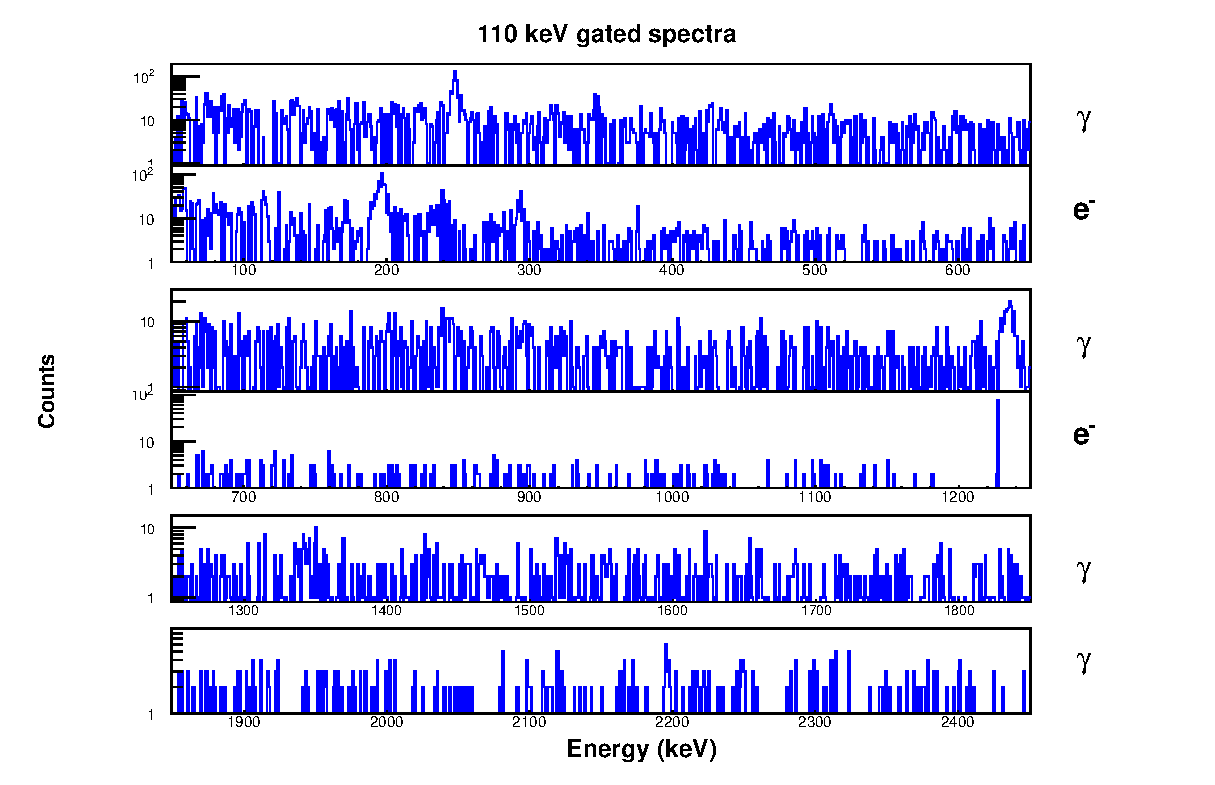
\includegraphics[scale=0.8]{154Gd_Appendix/110_combined.eps}
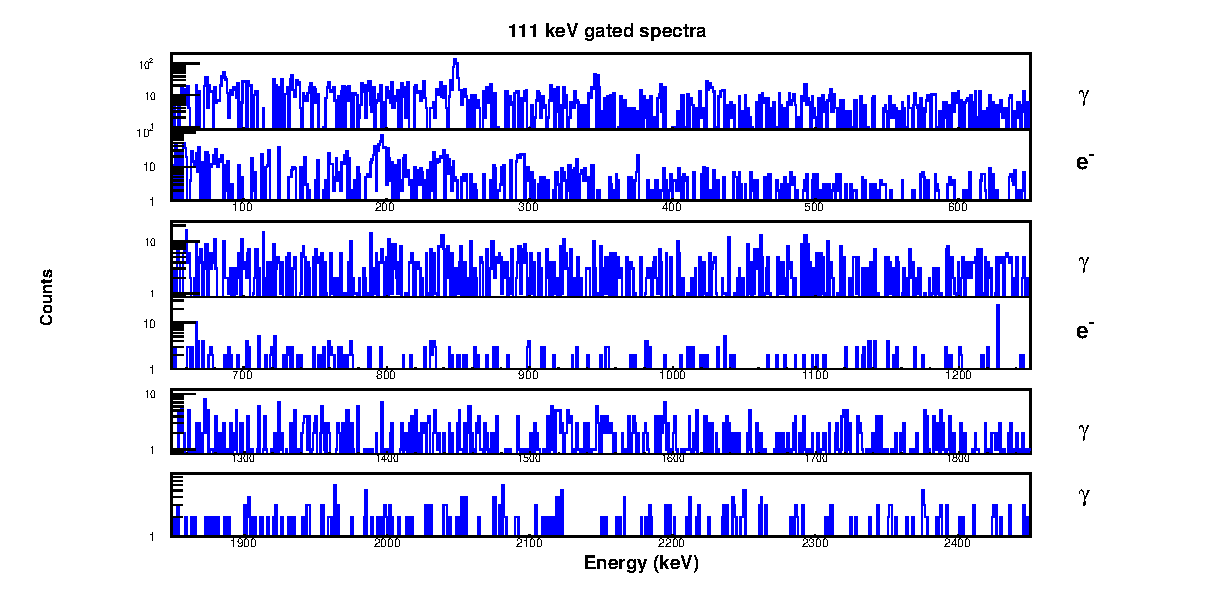
\includegraphics[scale=0.8]{154Gd_Appendix/111_combined.eps}
\includegraphics[scale=0.8]{154Gd_Appendix/123_combined.eps}
\includegraphics[scale=0.8]{154Gd_Appendix/134_combined.eps}
\includegraphics[scale=0.8]{154Gd_Appendix/141_combined.eps}
\includegraphics[scale=0.8]{154Gd_Appendix/162_combined.eps}
\includegraphics[scale=0.8]{154Gd_Appendix/165_combined.eps}
\includegraphics[scale=0.8]{154Gd_Appendix/167_combined.eps}
\includegraphics[scale=0.8]{154Gd_Appendix/171_combined.eps}
\includegraphics[scale=0.8]{154Gd_Appendix/181_combined.eps}
\includegraphics[scale=0.8]{154Gd_Appendix/188_combined.eps}
\includegraphics[scale=0.8]{154Gd_Appendix/192_combined.eps}
\includegraphics[scale=0.8]{154Gd_Appendix/199_combined.eps}
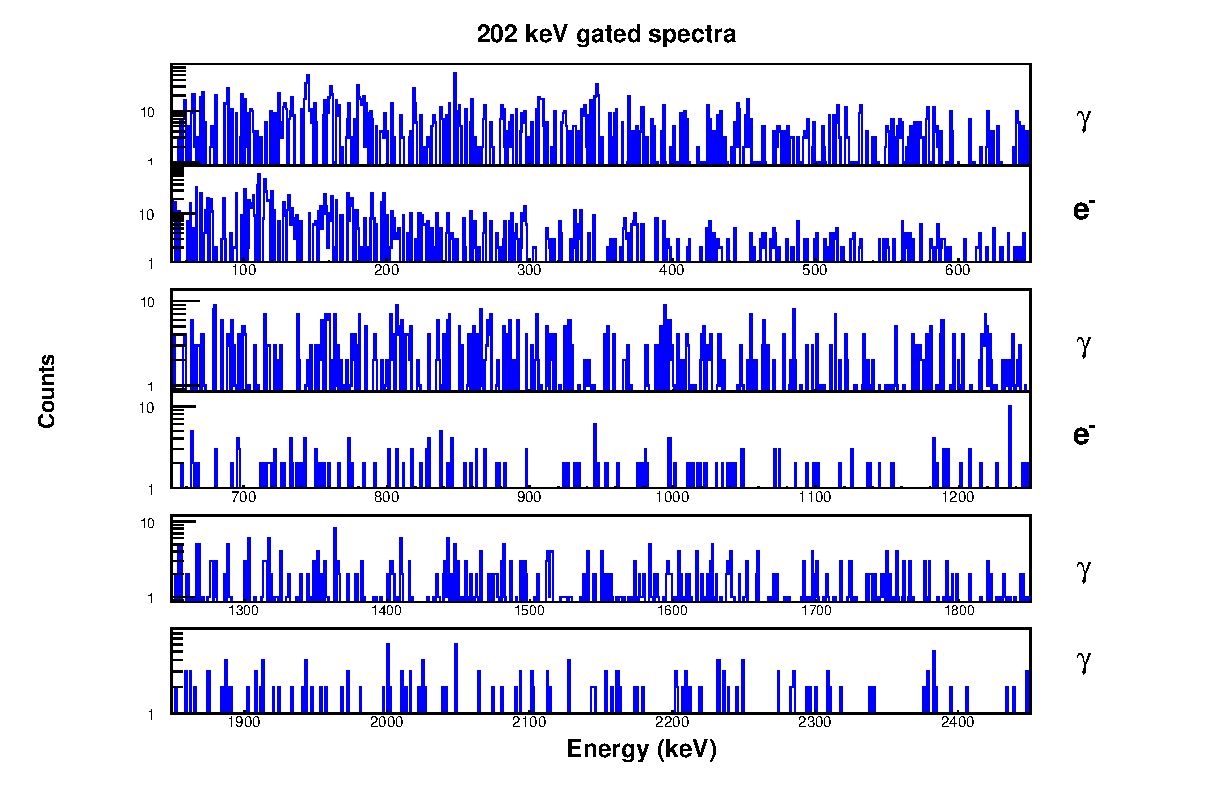
\includegraphics[scale=0.8]{154Gd_Appendix/202_combined.eps}
\includegraphics[scale=0.8]{154Gd_Appendix/210_combined.eps}
\includegraphics[scale=0.8]{154Gd_Appendix/218_combined.eps}
\includegraphics[scale=0.8]{154Gd_Appendix/224_combined.eps}
\includegraphics[scale=0.8]{154Gd_Appendix/227_combined.eps}
\includegraphics[scale=0.8]{154Gd_Appendix/232_combined.eps}
\includegraphics[scale=0.8]{154Gd_Appendix/235_combined.eps}
\includegraphics[scale=0.8]{154Gd_Appendix/238_combined.eps}
\includegraphics[scale=0.8]{154Gd_Appendix/247_combined.eps}
\includegraphics[scale=0.8]{154Gd_Appendix/265_combined.eps}
\includegraphics[scale=0.8]{154Gd_Appendix/267_combined.eps}
\includegraphics[scale=0.8]{154Gd_Appendix/274_combined.eps}
\includegraphics[scale=0.8]{154Gd_Appendix/282_combined.eps}
\includegraphics[scale=0.8]{154Gd_Appendix/285_combined.eps}
\includegraphics[scale=0.8]{154Gd_Appendix/297_combined.eps}
\includegraphics[scale=0.8]{154Gd_Appendix/303_combined.eps}
\includegraphics[scale=0.8]{154Gd_Appendix/306_combined.eps}
\includegraphics[scale=0.8]{154Gd_Appendix/315_combined.eps}
\includegraphics[scale=0.8]{154Gd_Appendix/318_combined.eps}
\includegraphics[scale=0.8]{154Gd_Appendix/325_combined.eps}
\includegraphics[scale=0.8]{154Gd_Appendix/333_combined.eps}
\includegraphics[scale=0.8]{154Gd_Appendix/339_combined.eps}
\includegraphics[scale=0.8]{154Gd_Appendix/343_combined.eps}
\includegraphics[scale=0.8]{154Gd_Appendix/346_combined.eps}
\includegraphics[scale=0.8]{154Gd_Appendix/381_combined.eps}
\includegraphics[scale=0.8]{154Gd_Appendix/390_combined.eps}
\includegraphics[scale=0.8]{154Gd_Appendix/408_combined.eps}
\includegraphics[scale=0.8]{154Gd_Appendix/412_combined.eps}
\includegraphics[scale=0.8]{154Gd_Appendix/417_combined.eps}
\includegraphics[scale=0.8]{154Gd_Appendix/426_combined.eps}
\includegraphics[scale=0.8]{154Gd_Appendix/435_combined.eps}
\includegraphics[scale=0.8]{154Gd_Appendix/437_combined.eps}
\includegraphics[scale=0.8]{154Gd_Appendix/451_combined.eps}
\includegraphics[scale=0.8]{154Gd_Appendix/465_combined.eps}
\includegraphics[scale=0.8]{154Gd_Appendix/467_combined.eps}
\includegraphics[scale=0.8]{154Gd_Appendix/471_combined.eps}
\includegraphics[scale=0.8]{154Gd_Appendix/480_combined.eps}
\includegraphics[scale=0.8]{154Gd_Appendix/492_combined.eps}
\includegraphics[scale=0.8]{154Gd_Appendix/501_combined.eps}
\includegraphics[scale=0.8]{154Gd_Appendix/505_combined.eps}
\includegraphics[scale=0.8]{154Gd_Appendix/508_combined.eps}
\includegraphics[scale=0.8]{154Gd_Appendix/557_combined.eps}
\includegraphics[scale=0.8]{154Gd_Appendix/568_combined.eps}
\includegraphics[scale=0.8]{154Gd_Appendix/577_combined.eps}
\includegraphics[scale=0.8]{154Gd_Appendix/596_combined.eps}
\includegraphics[scale=0.8]{154Gd_Appendix/598_combined.eps}
\includegraphics[scale=0.8]{154Gd_Appendix/600_combined.eps}
\includegraphics[scale=0.8]{154Gd_Appendix/604_combined.eps}
\includegraphics[scale=0.8]{154Gd_Appendix/612_combined.eps}
\includegraphics[scale=0.8]{154Gd_Appendix/630_combined.eps}
\includegraphics[scale=0.8]{154Gd_Appendix/637_combined.eps}
\includegraphics[scale=0.8]{154Gd_Appendix/642_combined.eps}
\includegraphics[scale=0.8]{154Gd_Appendix/648_combined.eps}
\includegraphics[scale=0.8]{154Gd_Appendix/650_combined.eps}
\includegraphics[scale=0.8]{154Gd_Appendix/654_combined.eps}
\includegraphics[scale=0.8]{154Gd_Appendix/676_combined.eps}
\includegraphics[scale=0.8]{154Gd_Appendix/680_combined.eps}
\includegraphics[scale=0.8]{154Gd_Appendix/682_combined.eps}
\includegraphics[scale=0.8]{154Gd_Appendix/685_combined.eps}
\includegraphics[scale=0.8]{154Gd_Appendix/692_combined.eps}
\includegraphics[scale=0.8]{154Gd_Appendix/696_combined.eps}
\includegraphics[scale=0.8]{154Gd_Appendix/722_combined.eps}
\includegraphics[scale=0.8]{154Gd_Appendix/724_combined.eps}
\includegraphics[scale=0.8]{154Gd_Appendix/758_combined.eps}
\includegraphics[scale=0.8]{154Gd_Appendix/761_combined.eps}
\includegraphics[scale=0.8]{154Gd_Appendix/797_combined.eps}
\includegraphics[scale=0.8]{154Gd_Appendix/811_combined.eps}
\includegraphics[scale=0.8]{154Gd_Appendix/834_combined.eps}
\includegraphics[scale=0.8]{154Gd_Appendix/837_combined.eps}
\includegraphics[scale=0.8]{154Gd_Appendix/840_combined.eps}
\includegraphics[scale=0.8]{154Gd_Appendix/842_combined.eps}
\includegraphics[scale=0.8]{154Gd_Appendix/844_combined.eps}
\includegraphics[scale=0.8]{154Gd_Appendix/850_combined.eps}
\includegraphics[scale=0.8]{154Gd_Appendix/874_combined.eps}
\includegraphics[scale=0.8]{154Gd_Appendix/891_combined.eps}
\includegraphics[scale=0.8]{154Gd_Appendix/894_combined.eps}
\includegraphics[scale=0.8]{154Gd_Appendix/904_combined.eps}
\includegraphics[scale=0.8]{154Gd_Appendix/962_combined.eps}
\includegraphics[scale=0.8]{154Gd_Appendix/996_combined.eps}
\includegraphics[scale=0.8]{154Gd_Appendix/1004_combined.eps}
\includegraphics[scale=0.8]{154Gd_Appendix/1021_combined.eps}
\includegraphics[scale=0.8]{154Gd_Appendix/1043_combined.eps}
\includegraphics[scale=0.8]{154Gd_Appendix/1059_combined.eps}
\includegraphics[scale=0.8]{154Gd_Appendix/1083_combined.eps}
\includegraphics[scale=0.8]{154Gd_Appendix/1127_combined.eps}
\includegraphics[scale=0.8]{154Gd_Appendix/1140_combined.eps}
\includegraphics[scale=0.8]{154Gd_Appendix/1194_combined.eps}
\includegraphics[scale=0.8]{154Gd_Appendix/1213_combined.eps}
\includegraphics[scale=0.8]{154Gd_Appendix/1217_combined.eps}
\includegraphics[scale=0.8]{154Gd_Appendix/1229_combined.eps}
\includegraphics[scale=0.8]{154Gd_Appendix/1237_combined.eps}
\includegraphics[scale=0.8]{154Gd_Appendix/1245_combined.eps}
\includegraphics[scale=0.8]{154Gd_Appendix/1303_combined.eps}
\includegraphics[scale=0.8]{154Gd_Appendix/1323_combined.eps}
\includegraphics[scale=0.8]{154Gd_Appendix/1339_combined.eps}
\includegraphics[scale=0.8]{154Gd_Appendix/1346_combined.eps}
\includegraphics[scale=0.8]{154Gd_Appendix/1370_combined.eps}
\includegraphics[scale=0.8]{154Gd_Appendix/1390_combined.eps}
\includegraphics[scale=0.8]{154Gd_Appendix/1421_combined.eps}
\includegraphics[scale=0.8]{154Gd_Appendix/1431_combined.eps}
\includegraphics[scale=0.8]{154Gd_Appendix/1450_combined.eps}
\includegraphics[scale=0.8]{154Gd_Appendix/1488_combined.eps}
\includegraphics[scale=0.8]{154Gd_Appendix/1514_combined.eps}
\includegraphics[scale=0.8]{154Gd_Appendix/1527_combined.eps}
\includegraphics[scale=0.8]{154Gd_Appendix/1572_combined.eps}
\includegraphics[scale=0.8]{154Gd_Appendix/1589_combined.eps}
\includegraphics[scale=0.8]{154Gd_Appendix/1658_combined.eps}
\includegraphics[scale=0.8]{154Gd_Appendix/1669_combined.eps}
\includegraphics[scale=0.8]{154Gd_Appendix/1671_combined.eps}
\includegraphics[scale=0.8]{154Gd_Appendix/1700_combined.eps}
\includegraphics[scale=0.8]{154Gd_Appendix/1713_combined.eps}
\includegraphics[scale=0.8]{154Gd_Appendix/1788_combined.eps}
\includegraphics[scale=0.8]{154Gd_Appendix/1810_combined.eps}
\includegraphics[scale=0.8]{154Gd_Appendix/1895_combined.eps}
\includegraphics[scale=0.8]{154Gd_Appendix/1940_combined.eps}
\includegraphics[scale=0.8]{154Gd_Appendix/2007_combined.eps}
\includegraphics[scale=0.8]{154Gd_Appendix/2025_combined.eps}
\includegraphics[scale=0.8]{154Gd_Appendix/2173_combined.eps}
\includegraphics[scale=0.8]{154Gd_Appendix/2310_combined.eps}
\includegraphics[scale=0.8]{154Gd_Appendix/2435_combined.eps}
\includegraphics[scale=0.8]{154Gd_Appendix/2628_combined.eps}
\includegraphics[scale=0.8]{154Gd_Appendix/2648_combined.eps}
\includegraphics[scale=0.8]{154Gd_Appendix/2682_combined.eps}
%\end{landscape}
%\chapter{$^{156}$Gd Gated Spectra}
\label{chap:156_spectra}

The following is a compendium of spectra from the gates on the $^{156}$Gd data. A table with the gates and the corresponding background gates used in subtraction is listed. Unless noted, the energy listed is the center of the gate, with a range of $\pm$1.5 keV.

\begin{longtable}{>{\centering\arraybackslash}p{0.15\textwidth}|>{\centering\arraybackslash}p{0.15\textwidth}|p{0.6\textwidth}}
    \caption{List of $^{156}$Gd gates}
    \label{tab:1546d_gates} \\
    \toprule
    $E_{gate}$ (keV) & $E_{bkgd}$ (keV) & Description \\ \hline
    \endfirsthead
    \caption[]{List of $^{156}$Gd gates} \\
    \toprule
    $E_{gate}$ (keV) & $E_{bkgd}$ (keV) & Description \\ \hline
    \endhead
      89 & 100 & $2^+_{gs}\rightarrow0^+_{gs}$\\ \hline
      110.6 & 120 & $5^+_{}\rightarrow4^+_{}$ in $K^{\pi}=4^+$ band\\ \hline
      156.7 & 175 & $7^+_{}\rightarrow6^+_{}$ in $K^{\pi}=4^+$ band\\ \hline
      199.2 & 215 & $4^+_{gs}\rightarrow2^+_{gs}$\\ \hline
      227.4 & 250 & $7^-_{}\rightarrow7^+_{}$ with $7^+$ in $K^{\pi}=4^+$ band\\ \hline
      287.6 & 310 & $6^+_{\gamma}\rightarrow4^+_{\gamma}$\\ \hline
      296.5 & 310 & $6^+_{gs}\rightarrow4^+_{gs}$\\ \hline
      322.1 & 350 & $8^-_{}\rightarrow6^-_{}$ in $K^{pi}=1^-$ octopole-vibrational band\\ \hline
      357.7 & 370 & $4^+_{}\rightarrow2^+_{gs}$ with $4^+$ in $K^{\pi}=4^+$ band\\ \hline
      380.4 & 390 & $8^+_{gs}\rightarrow6^+_{gs}$\\ \hline
      399.9 & 410 & $9^+_{\gamma}\rightarrow7^+_{\gamma}$\\ \hline
      451 & 465 & $10^+_{gs}\rightarrow8^+_{gs}$\\ \hline
      568.3 & 640 & $2^-_{}\rightarrow1^-_{}$ with $2^-$ in $K^{\pi}=2^-$ and $1^-$ in $K^{\pi}=0^-$ octopole vibrational bands. \\ \hline
      789.7 & 795 & $3^-+_{}\rightarrow4^-_{}$ with $3^+$ in $K^{\pi}=1^+$ band and $4^-$ in $K^{\pi}=1^-$ octopole vibrational band\\ \hline
      823.6 & 900 & $5^-_{}\rightarrow6^+_{gs}$ with $5^-$ in $K^{\pi}=1^-$ octopole vibrational band\\ \hline
      875.9 & 900 & $4^+_{3}\rightarrow6^+_{gs}$ with $4^+$ in $2^{nd}$ excited $0^+$ band\\ \hline
      883.6 & 900 & $8^+_{2}\rightarrow8^+_{gs}$ with $8^+$ in $1^{st}$ excited $0^+$ band and $7^+_{\gamma}\rightarrow8^+_{gs}$\\ \hline
      922.6 & 1000 & $5^+_{\gamma}\rightarrow6^+_{gs}$\\ \hline
      943.6 & 980 & $7^+_{}\rightarrow8^+_{gs}$ with $7^+$ in $K^{\pi}=4^+$ band\\ \hline
      954.5 & 1000 & $6^+_{2}\rightarrow6^+_{gs}$ with $6^+$ in $1^{st}$ excited $0^+$ band\\ \hline
      960.2 & 980 & $3^+_{\gamma}\rightarrow4^+_{\gamma}$\\ \hline
      969.2 & 980 & $2^+_{3}\rightarrow4^+_{gs}$ with $2^+$ in $2^{nd}$ excited $0^+$ band\\ \hline
      988 & 1000 & $3^-_{}\rightarrow4^+_{gs}$ with $3^-$ in $K^{\pi}=1^-$ octopole vibrational band\\ \hline
      992.8 & 1000 & $9^-_{}\rightarrow8^+_{gs}$ with $9^-$ in $K^{\pi}=1^-$ octopole vibrational band\\ \hline
      1010.7 & 1100 & $4^+_{2}\rightarrow4^+_{gs}$ with $4^+$ in $1^{st}$ excited $0^+$ band\\ \hline
      1013.3 & 1100 & Likely a transition into $10^+_{gs}$\\ \hline
      1039.4 & 1100 & $5^+_{}\rightarrow6^+_{gs}$ with $5^+$ in $K^{\pi}=4^+$ band\\ \hline
      1044.5 & 1090 & $8^+{\gamma}\rightarrow8^+_{gs}$\\ \hline
      1052.2 & 1100 & $7^-_{}\rightarrow6^+_{gs}$ with $7^-$ in $K^{\pi}=1^-$ band\\ \hline
      1058.5 & 1090 & $6^+{\gamma}\rightarrow6^+_{gs}$\\ \hline
      1067.5 & 1100 & $4^+{\gamma}\rightarrow4^+_{gs}$ and $2^+{\gamma}\rightarrow2^+_{gs}$\\ \hline
      1119.2 & 1150 & $6^-{}\rightarrow6^+_{gs}$ with $6^-$ in $K^{\pi}=1^-$ octopole vibrational band\\ \hline
      1156.8 & 1200 & $1^-{}\rightarrow2^+_{gs}$ with $1^-$ in $K^{\pi}=1^-$ octopole vibrational band and $2^+_{2}\rightarrow0^+_{gs}$ with $2^+$ in $1^{st}$ excited $0^+$ band\\ \hline
      1168.2 & 1200 & $2^+_{3}\rightarrow2^+_{gs}$ with $2^+$ in $2^{nd}$ excited $0^+$ band and $0^+_{3}\rightarrow0^+_{gs}$ gamma-equivalent\\ \hline
      1180.6 & 1200 & $6^+_{3}\rightarrow6^+_{gs}$ with $2^+$ in $2^{nd}$ excited $0^+$ band\\ \hline
      1188.3 & 1200 & $3^-{}\rightarrow2^+_{gs}$ with $1^-$ in $K^{\pi}=1^-$ octopole vibrational band \\ \hline
      1221.7 & 1240 & $4^+_{}\rightarrow4^+_{gs}$ with $4^+$ in $K^{\pi}=4^+$ band\\ \hline
      1250 & 1300 & $3^-{}\rightarrow4^+_{gs}$ with $3^-$ in $K^{\pi}=0^-$ octopole vibrational band\\ \hline
      1265.1 & 1300 & $7^+_{\gamma}\rightarrow6^+_{gs}$ and $8^+_{2}\rightarrow6^+_{gs}$ with $8^+$ in $1^{st}$ excited $0^+$ band\\ \hline
      1284.7 & 1300 & $9^+_{\gamma}\rightarrow6^+_{gs}$\\ \hline
      1325.8 & 1400 & $7^+_{}\rightarrow6^+_{gs}$ with $7^+$ in $K^{\pi}=4^+$ band\\ \hline
      1334.9 & 1348 & $5^+_{}\rightarrow4^+_{gs}$ with $5^+$ in $K^{\pi}=4^+$ band\\ \hline
      1355.9 & 1400 & $6^+_{\gamma}\rightarrow4^+_{gs}$ \\ \hline
      1479.7 & 1500 & $10^+_{\gamma}\rightarrow8^+_{gs}$ and $6^+_{3}\rightarrow4^+_{gs}$ with $6^+$ in $2^{nd}$ excited $0^+$ band\\ \hline
      1494 & 1500 & No known transitions in agreement, but appears in coincidence with ground state band transitions.\\ \hline
      1605 & 1630 & $4^+_{4}\rightarrow4^+_{gs}$ with $4^+$ in $3^{rd}$ excited $0^+$ band\\ \hline
      1731.1 & 1750 & $4^+_{4}\rightarrow4^+_{gs}$ with $4^+$ in $K^{\pi}=2^+$ band\\
    \bottomrule
\end{longtable}

\pagebreak

\begin{figure}
    \caption{Spectra for the gates listed in Table \ref{tab:156Gd_gates}, in numerical order, spanning pages 396-441.}
    \label{fig:156_App}
\end{figure}

\pagebreak

\begin{landscape}
\includegraphics[scale=1.2]{156Gd_Appendix/89_combined.eps}
\includegraphics[scale=1.2]{156Gd_Appendix/110_combined.eps}
\includegraphics[scale=1.2]{156Gd_Appendix/156_combined.eps}
\includegraphics[scale=1.2]{156Gd_Appendix/199_combined.eps}
\includegraphics[scale=1.2]{156Gd_Appendix/227_combined.eps}
\includegraphics[scale=1.2]{156Gd_Appendix/287_combined.eps}
\includegraphics[scale=1.2]{156Gd_Appendix/296_combined.eps}
\includegraphics[scale=1.2]{156Gd_Appendix/322_combined.eps}
\includegraphics[scale=1.2]{156Gd_Appendix/357_combined.eps}
\includegraphics[scale=1.2]{156Gd_Appendix/380_combined.eps}
\includegraphics[scale=1.2]{156Gd_Appendix/399_combined.eps}
\includegraphics[scale=1.2]{156Gd_Appendix/451_combined.eps}
\includegraphics[scale=1.2]{156Gd_Appendix/568_combined.eps}
\includegraphics[scale=1.2]{156Gd_Appendix/789_combined.eps}
\includegraphics[scale=1.2]{156Gd_Appendix/823_combined.eps}
\includegraphics[scale=1.2]{156Gd_Appendix/875_combined.eps}
\includegraphics[scale=1.2]{156Gd_Appendix/883_combined.eps}
\includegraphics[scale=1.2]{156Gd_Appendix/922_combined.eps}
\includegraphics[scale=1.2]{156Gd_Appendix/943_combined.eps}
\includegraphics[scale=1.2]{156Gd_Appendix/954_combined.eps}
\includegraphics[scale=1.2]{156Gd_Appendix/960_combined.eps}
\includegraphics[scale=1.2]{156Gd_Appendix/969_combined.eps}
\includegraphics[scale=1.2]{156Gd_Appendix/988_combined.eps}
\includegraphics[scale=1.2]{156Gd_Appendix/992_combined.eps}
\includegraphics[scale=1.2]{156Gd_Appendix/1010_combined.eps}
\includegraphics[scale=1.2]{156Gd_Appendix/1013_combined.eps}
\includegraphics[scale=1.2]{156Gd_Appendix/1039_combined.eps}
\includegraphics[scale=1.2]{156Gd_Appendix/1044_combined.eps}
\includegraphics[scale=1.2]{156Gd_Appendix/1052_combined.eps}
\includegraphics[scale=1.2]{156Gd_Appendix/1058_combined.eps}
\includegraphics[scale=1.2]{156Gd_Appendix/1067_combined.eps}
\includegraphics[scale=1.2]{156Gd_Appendix/1119_combined.eps}
\includegraphics[scale=1.2]{156Gd_Appendix/1156_combined.eps}
\includegraphics[scale=1.2]{156Gd_Appendix/1168_combined.eps}
\includegraphics[scale=1.2]{156Gd_Appendix/1180_combined.eps}
\includegraphics[scale=1.2]{156Gd_Appendix/1221_combined.eps}
\includegraphics[scale=1.2]{156Gd_Appendix/1250_combined.eps}
\includegraphics[scale=1.2]{156Gd_Appendix/1265_combined.eps}
\includegraphics[scale=1.2]{156Gd_Appendix/1284_combined.eps}
\includegraphics[scale=1.2]{156Gd_Appendix/1325_combined.eps}
\includegraphics[scale=1.2]{156Gd_Appendix/1334_combined.eps}
\includegraphics[scale=1.2]{156Gd_Appendix/1355_combined.eps}
\includegraphics[scale=1.2]{156Gd_Appendix/1479_combined.eps}
\includegraphics[scale=1.2]{156Gd_Appendix/1491_combined.eps}
\includegraphics[scale=1.2]{156Gd_Appendix/1605_combined.eps}
\includegraphics[scale=1.2]{156Gd_Appendix/1731_combined.eps}
\end{landscape}
%%
% Modified by Megan Patnott
% Last Change: Jan 18, 2013
%
%%%%%%%%%%%%%%%%%%%%%%%%%%%%%%%%%%%%%%%%%%%%%%%%%%%%%%%%%%%%%%%%%%%%%%%%
%
% Modified by Sameer Vijay
% Last Change: Tue Jul 26 2005 13:00 CEST
%
%%%%%%%%%%%%%%%%%%%%%%%%%%%%%%%%%%%%%%%%%%%%%%%%%%%%%%%%%%%%%%%%%%%%%%%%
%
% Sample Notre Dame Thesis/Dissertation
% Using Donald Peterson's ndthesis classfile
%
% Written by Jeff Squyres and Don Peterson
%
% Provided by the Information Technology Committee of
%   the Graduate Student Union
%   http://www.gsu.nd.edu/
%
% Nothing in this document is serious except the format.  :-)
%
% If you have any suggestions, comments, questions, please send e-mail
% to: ndthesis@gsu.nd.edu
%
%%%%%%%%%%%%%%%%%%%%%%%%%%%%%%%%%%%%%%%%%%%%%%%%%%%%%%%%%%%%%%%%%%%%%%%%


%
% Appendix for Analysis Code
%

\chapter{Analysis Code}
\label{chap:code}

This appendix contains the analysis code used to gate on rootfiles. It was compiled using ROOT 5.34.19, and later ROOT 6.02 libraries. The GCC compiler version 7.1.0. Included in this appendix are the makefiles and example input files for parameters.

There are two codes used for analysis: the coincidence gating, and the code to merge the analysis of the individual runs together. These two codes were written to share multiple elements. The code in this appendix is broken into four sections: the code unique to the coincidence gating, the code unique to the merge code, the shared code between the two, and example input files from the \texttt{user} folder.

The folder structure for the code is in the following list. Some files listed are not used in the merge code, and would not be present in the directory. The topmost bullets are all in the main code directory. 

\begin{itemize}[noitemsep, nolistsep]
    \item README.md
    \item Makefile
    \item QueueScript.sh
    \item include
    \vspace{-5mm}\begin{itemize}[noitemsep, nolistsep, topsep=0pt, label=\textbullet]
        \item Coefficients.h
        \item Constraints.h
        \item Filelist.h
        \item analysis.h
        \item histograms.h
        \item timing.h
    \end{itemize}
    \item logs
    \item src
    \vspace{-5mm}\begin{itemize}[noitemsep, nolistsep, topsep=0pt, label=\textbullet]
        \item Coefficients.cxx
        \item Constraints.cxx
        \item Filelist.cxx
        \item analysis.cxx
        \item histograms.cxx
        \item main.cxx
        \item timing.cxx
    \end{itemize}
    \item user
    \vspace{-5mm}\begin{itemize}[noitemsep, nolistsep, topsep=0pt, label=\textbullet]
        \item BGO.dat
        \item Cut\_Files
        \vspace{-5mm}\begin{itemize}[noitemsep, nolistsep, topsep=0pt, label=\textbullet]
            \item GeCut.dat
            \item SiLiCut.dat
        \end{itemize}
        \item Filelist.dat
        \item GeCoefficients.dat
        \item Run\_by\_Run
        \vspace{-5mm}\begin{itemize}[noitemsep, nolistsep, topsep=0pt, label=\textbullet]
            \item GeCoefficients\_r*.dat
            \item SiLiCoefficients\_r*.dat
        \end{itemize}
        \item SiLiCoefficients.dat
        \item Timing.dat
    \end{itemize}
\end{itemize}

Please note, "logs" is an otherwise empty folder that is used for putting output files from running code on the CRC backend. Should one wish to run code locally in the terminal window, this folder would be unnecessary, and the shell script named "QueueScript.sh" would be adjusted for local use.

\section{Coincidence Code}

The code in this appendix is expressly for the ICEBall-GEORGINA data. The ICEBall-Clovershare data used a different version of the \texttt{evt2root} converter, which no longer required the \texttt{libExpEvent.so} that was generated by the converter. The \texttt{analysis.cxx} file was also changed to reflect the different tree structure created by the converter. While not replicated here, the area of change is referred to in that subsection.

\includecode{md}{README.md}{README.md}{Simple included explanation of code inputs for running.}

\includecode{make}{Makefile}{Makefile}{In this code, CodeDirectory must be replaced with the path to the code directory. \mint{make}|-L/CodeDirectory/libExpEvent.so| could be removed in the Clovershare data due to the converter changes.}

\includecode{bash}{Queuescript.sh}{Queuescript.sh}{This shell script is written for executing the code on the CRC backend computers. It can be used locally by removing the commented lines down to line 9, and replacing \mint{bash}|$SGE_TASK_ID| with the run number. The terms "netID","Nickname","runStart","runEnd", "CodeDirectory","FileOut", "CutFile", and "TimingFile" must all be replaced with the correct information.}

\includecode{c++}{src/main.cxx}{src/main.cxx}{This is the main code that calls all of the subroutines. The gSystem line is necessary to load the library to read the tree structure of the root files. "Directory" and "OutputDirectory" should be replaced with the proper filepaths.}

\includecode{c++}{src/analysis.cxx}{src/analysis.cxx}{This is the main analysis section of the code. The skeleton is built using the MakeClass routine in ROOT.\citep{brun97:_root} If the structure of the tree varies, this is where the changes would reflect, from lines \texttt{154}-\texttt{206}, where the event tree values are assigned to local variables for manipulation in the code.}

\subsection{\texttt{src/analysis.h}}

This header file has not been included, as it is procedurally generated by the MakeClass routine in ROOT. It changes based on the tree directory.

\includecode{c++}{src/histograms.cxx}{src/histograms.cxx}{These are the subroutines for the creation, adding to, and writing to file of the histograms created in the gating process.}

\includecode{c++}{include/histograms.h}{include/histograms.h}{Header file for \texttt{histograms.cxx}.}

\includecode{c++}{src/timing.cxx}{src/timing.cxx}{This is a class for keeping track of the timing gates used between pairs of detectors.}

\includecode{c++}{include/timing.h}{include/timing.h}{Header file for \texttt{timing.cxx}.}

\section{Merge Code}

\includecode{md}{merge/README.md}{README.md}{Simple included explanation of code inputs for running. Includes important commentary on inputs when used in conjunction with the coincidence code.}

\includecode{make}{merge/Makefile}{Makefile}{The compilation code.}

\includecode{c++}{merge/main.cxx}{src/main.cxx}{This is the main code that calls all the subroutines. The main subroutine used is in the histograms code. "\$OutputDirectory\$ must be replaced with the output directory.}

\includecode{c++}{merge/histograms.cxx}{src/histograms.cxx}{This is the code that combines the histograms of the separate files into one.}

\includecode{c++}{merge/histograms.h}{include/histograms.h}{Header file for \texttt{histograms.cxx}.}

\section{Code Shared between Coincidence and Merge}

\includecode{c++}{src/Coefficients.cxx}{src/Coefficients.cxx}{These are the subroutines for reading in calibration coefficients for the Si(Li) and HPGe detectors.}

\includecode{c++}{include/Coefficients.h}{include/Coefficients.h}{Header file for \texttt{Coefficients.cxx}.}

\includecode{c++}{src/Constraints.cxx}{src/Constraints.cxx}{These are the subroutines for reading in coincidence gates for the BGO, Si(Li), and HPGe detectors.}

\includecode{c++}{include/Constraints.h}{include/Constraints.h}{Header file for \texttt{Constraints.cxx}.}

\includecode{c++}{src/Filelist.cxx}{src/Filelist.cxx}{These are the subroutines for reading in the directory to the data, the generalized run name, the file type, and the tree name. The tree name is not used in the merge code.}

\includecode{c++}{include/Filelist.h}{include/Filelist.h}{Header file for \texttt{Filelist.cxx}.}

\section{Example User Files}

\includecode{c++}{user/Filelist.dat}{user/Filelist.dat}{This is read in by the \texttt{Filelist.cxx} subroutines. It includes the path to the raw data files, the name of the tree, and the formatting for the beginning and end of the data files, including the file extension. "DataDirectory" should be replaced with the correct filepath. The comments must be left in for proper spacing to be read by the program.}

\includecode{c++}{user/GeCoefficients.dat}{user/GeCoefficients.dat}{This is read in by the \texttt{Coefficients.cxx} subroutines. It includes the number of HPGe detectors, the polynomial order of the energy calibration, and the energy calibration itself. Coefficients are in order of increasing polynomial ($0^{th}$, $1^{st}$, etc.). It also is set up for segmented detectors, as in the Clovershare runs. In the case of the different tree structure in the Clovershare data, it also contains the start index of the HPGe detectors in the \texttt{evt} tree array. As a special correction function was used on the residuals to deal with the differential non-linearity of the electronics, as discussed in section \ref{sec:clover_electronics} and \ref{sec:non-linearity}, these coefficients are also included. They can be excluded if not needed. The comments must be left in for proper spacing to be read by the program.}

\includecode{c++}{user/SiLiCoefficients.dat}{user/SiLiCoefficients.dat}{This is read in by the \texttt{Coefficients.cxx} subroutines. It includes the number of Si(Li) detectors, the polynomial order of the energy calibration, and the energy calibration itself. Coefficients are in order of increasing polynomial ($0^{th}$, $1^{st}$, etc.). In the case of the different tree structure in the Clovershare data, it also contains the start index  of the Si(Li) detectors in the \texttt{evt} tree array. The comments must be left in for proper spacing to be read by the program.}

\includecode{c++}{user/BGO.dat}{user/BGO.dat}{This is read in by the \texttt{Coefficients.cxx} subroutines. It includes the number of BGO detectors and the thresholds for each detector. In the case of the different tree structure in the Clovershare data, it also contains the start index  of the BGO detectors in the \texttt{evt} tree array. The comments must be left in for proper spacing to be read by the program.}

\includecode{c++}{user/Timing.dat}{user/Timing.dat}{This is read in by the \texttt{Timing.cxx} subroutines. It includes the timing cut for each pairing of detectors. Each pairing has index of each detector and the upper and lower limit of the timing gate. Indexes for detectors start at 0. If the number of detectors is incorrect in either the \texttt{GeCoefficients.cxx} or the \texttt{SiLiCoefficients.cxx}, this file will not be read in correctly. The order of pairing groups (ge-ge, ge-sili, etc.) must be kept the same. The comments must be left in for proper spacing to be read by the program. This file name can be changed so multiple timing files can exist, as the timing file is specified as input when running the program.}

\includecode{c++}{user/Cut_Files/GeCuts.dat}{user/Cut\_Files/GeCuts.dat}{This is read in by the \texttt{Constraints.cxx} subroutines. It includes the number cuts to run on the HPGe detectors. Each cut is then listed as the detector index, the center of the gate, and half the width of the gate. This is done to mirror the centroid and width of peaks, for readability. The comments must be left in for proper spacing to be read by the program. This file name can be changed so multiple timing files can exist, as the timing file is specified as input when running the program.}

\includecode{c++}{user/Cut_Files/SiLiCuts.dat}{user/Cut\_Files/SiLiCuts.dat}{This is read in by the \texttt{Constraints.cxx} subroutines. It includes the number cuts to run on the HPGe detectors. Each cut is then listed as the detector index, the center of the gate, and half the width of the gate. This is done to mirror the centroid and width of peaks, for readability. The comments must be left in for proper spacing to be read by the program. This file name can be changed so multiple timing files can exist, as the timing file is specified as input when running the program.}

\includecode{c++}{user/Run_by_Run/GeCoefficients.dat}{user/Run\_by\_Run/GeCoefficients\_r*.dat}{This is read in by the \texttt{Coefficients.cxx} subroutines. It includes a linear correction for the HPGe detectors based on the run specified where * is in the file name. The run correction is assumed to be linear, and the number of detectors is assumed from the base calibration files. The comments must be left in for proper spacing to be read by the program. This file name can be changed so multiple run files can exist, as the run file is based on the run being analyzed. These files can be excluded and the correction will be set to y=x automatically.}

%\includecode{c++}{}{user/Run\_by\_Run/SiLiCoefficients\_r*.dat}{This is read in by the \texttt{Coefficients.cxx} subroutines. It includes a linear correction for the Si(Li) detectors based on the run specified where * is in the file name. The run correction is assumed to be linear, and the number of detectors is assumed from the base calibration files. The comments must be left in for proper spacing to be read by the program. This file name can be changed so multiple run files can exist, as the run file is based on the run being analyzed. These files can be excluded and the correction will be set to y=x automatically.}
%%
% Modified by Megan Patnott
% Last Change: Jan 18, 2013
%
%%%%%%%%%%%%%%%%%%%%%%%%%%%%%%%%%%%%%%%%%%%%%%%%%%%%%%%%%%%%%%%%%%%%%%%%
%
% Modified by Sameer Vijay
% Last Change: Tue Jul 26 2005 13:00 CEST
%
%%%%%%%%%%%%%%%%%%%%%%%%%%%%%%%%%%%%%%%%%%%%%%%%%%%%%%%%%%%%%%%%%%%%%%%%
%
% Sample Notre Dame Thesis/Dissertation
% Using Donald Peterson's ndthesis classfile
%
% Written by Jeff Squyres and Don Peterson
%
% Provided by the Information Technology Committee of
%   the Graduate Student Union
%   http://www.gsu.nd.edu/
%
% Nothing in this document is serious except the format.  :-)
%
% If you have any suggestions, comments, questions, please send e-mail
% to: ndthesis@gsu.nd.edu
%
%%%%%%%%%%%%%%%%%%%%%%%%%%%%%%%%%%%%%%%%%%%%%%%%%%%%%%%%%%%%%%%%%%%%%%%%


%
% Appendix for Analysis Code
%

\chapter{ROOT Macro Codes}
\label{chap:macro}

This appendix contains macros used in ROOT for various pieces of analysis, such as subtracting off peaks or piecewise background fits. All codes were run using ROOT version 5.34.19 \citep{brun97:_root}.

\includemacro{c++}{FitterProgram.cxx}{FitterProgram.cxx}{This code is a series of fitting macros for various kinds of spectra and peak types. These fits were compared with RADWARE\citep{radford00:_radware} for consistency.}

\includemacro{c++}{skewedsubtraction.cxx}{skewedsubtraction.cxx}{This code is used for subtracting off conversion electron peaks, typically those from the ground state band in this work, from the conversion electron spectrum to look for smaller peaks and upper limits.}

\includemacro{c++}{Piecewise_macro.cxx}{Piecewise\_macro.cxx}{This code was used for fitting the background on either side of a peak and outputting the area under the peak after subtracting the background off. It must be compiled by root for use by being converted into a shared library by ACLiC.}

\includemacro{c++}{ROOT2SPE.cxx}{ROOT2SPE.cxx}{This code was used for converting ROOT histograms into \texttt{.spe} files for use by RADWARE \citep{radford00:_radware}. It uses an existing conversion in the RADWARE source code to convert from \texttt{ascii} to \texttt{spe}.}


%
% Back stuff
%

% % comment out the following three lines
% if using chapter-wise bibliography

 \backmatter
 \bibliographystyle{abbrvnat} % The standard abbrvnat style should be acceptable. Also provided with both the advanced and standard
 \bibliography{Bibliography}       % distributions are nddiss2e and nddiss2enoarticletitles style options.
% If you prefer to manually enter your bibliography, that is fine. Comment out the previous two lines, and enter your bibliography
% as usual. Note that if you choose this route, formatting the bibliography is your responsibility. An example is below, including the
% optional arguments necessary for author-date style citations.
%	\begin{thebibliography}{9}
%		\bibitem[Galmira(1998)]{galmira98:_gnus_milit} G.\ Galmira. Gnus and the military -- a secret conspiracy? \emph{Growing Towards Gnu}, III(7):22--183, September 1998.
%		
%		\bibitem[Ganston and Greenfield(1998)]{gnus98:_gerry_ganst} G.\ Ganston and G.\ Greenfield. \emph{Gnus and You: The Art of Being New}. volume I. Grapping Books, NY, August, 1998.
%		
%		\bibitem[Gloonston(1998)]{gloonston98:_gnuly_discov_gnus} G.\ Gloonston. Newly discovered gnus: The LoG. \emph{Growing Towards Gnu}, II(12):23---57, March 1998.
%		
%		\bibitem[Greenfield(1996)]{greenfield96:_gettin_know_gnu} G.\ Greenfield. \emph{Getting to Know Gnu}. PhD thesis, Geoffrey Garfield School of Gnus, August 1996.
%		
%		\bibitem[van Gairley(2000)]{gairley2000} G.\ van Gairley. Gnu's review. Website, 2000. \url{http://www.gairley.gnu}.
%	\end{thebibliography}

\end{document}

% End of ``example.tex''
